% chktex: 2/9/12/13/17/25 disabled file-wide --- as of 2026-07-19 all instances fire only in
% the verbatim Part II archive (interval notation [0,1), archival prose); Part I is clean.
% chktex-file 2
% chktex-file 9
% chktex-file 12
% chktex-file 13
% chktex-file 17
% chktex-file 25
\documentclass[11pt]{article}

\usepackage[margin=1in]{geometry}
\usepackage{amsmath}
\usepackage{amssymb}
\usepackage{amsthm}
\usepackage{booktabs}
\usepackage{float}
\usepackage{enumitem}
\usepackage{xcolor}
\usepackage{tcolorbox}
\usepackage{pgfplots}
\pgfplotsset{compat=1.18}
\usepackage[round]{natbib}
\usepackage[hidelinks]{hyperref}

\theoremstyle{plain}
\newtheorem{proposition}{Proposition}
\newtheorem{lemma}{Lemma}
\newtheorem{corollary}{Corollary}
\newtheorem{assumption}{Assumption}

\theoremstyle{remark}
\newtheorem{remark}{Remark}

\title{Model 2.0}
\author{}
\date{\today}

% Part II (disparity note) support, ported verbatim from model_companion_disparity.tex.
\definecolor{csframe}{RGB}{0,90,140}
\definecolor{csback}{RGB}{242,248,252}
\newtcolorbox{csbox}{colback=csback,colframe=csframe,boxrule=0.6pt,arc=2pt,left=6pt,right=6pt,top=2pt,bottom=2pt}
\newcommand{\R}{\mathbb R}
\newcommand{\wS}{\omega^S}
\newcommand{\wR}{\omega^R}
\newcommand{\what}{\hat\omega^R}
\newcommand{\sgn}{\operatorname{sign}}
\newcommand{\argmax}{\operatorname*{arg\,max}}

\begin{document}

\maketitle

\part*{Part I. Model 2.0}

\section{How Representations Shape Strategic Behavior}
\label{sec:behavior}

Two players interact once. Player $S$ is the first mover---the dictator, the proposer, the investor; generically, the \emph{sender}---and player $R$ is the second mover or \emph{receiver}. The sender's initial wealth is normalized to one, and her action is the share $t\in[0,1]$ she sends to the receiver. Total final wealth is $W(t)$, which may depend on the amount sent, $\pi_S$ denotes the sender's material payoff, and $\pi_R$ denotes the receiver's material payoff.

A \emph{representation} of the game is a pair $\mathbf{r}=(\boldsymbol{\alpha},\mathbf{x})$: an attention profile $\boldsymbol{\alpha}=(\rho,\sigma,\mu)$ over payoff elements and, in the strategic games, a believed behavior $\mathbf{x}$ of the receiver. Given her representation, the sender maximizes
\begin{equation}
u_S (t) \;=\; \rho\, W(t)\;-\;\sigma\, \pi_R\;-\;\frac{\mu}{2}\left(t-t^{e}\right)^{2},
\label{eq:utility}
\end{equation}
where the three payoff elements are total wealth, the receiver's material payoff, and a sharing norm anchored at the \emph{equal-payoff action} $t^{e}$---the action that equalizes the two players' material payoffs under the sender's representation: the equal split $t^{e}=\tfrac12$ in the dictator and ultimatum games and, in the trust game, where the multiplier breaks that coincidence, the send that equalizes expected payoffs at the believed return (Proposition~\ref{prop:tg}). The Greek letters are attention weights, with $\rho=\sigma=\mu=1$ the undistorted case in which no motive is slanted by the representation and the sender has inequity-averse utility in the spirit of \citet{BoltonOckenfels2000}. Standard models prescribe \emph{stability}---that is, an attention profile that stays fixed while context varies---and, in the strategic games, \emph{rational expectations}---that is, beliefs that track actual behavior. 

Because $\pi_S=W(t)-\pi_R$, equation~\eqref{eq:utility} can be rewritten as
\begin{equation}
u_S(t) \;=\; \sigma\,\pi_S \;+\; (\rho-\sigma)\,W(t)\;-\;\frac{\mu}{2}\left(t-t^{e}\right)^{2},
\label{eq:utility_rewritten}
\end{equation}
which makes the mapping to motives transparent: $\sigma$ is attention to own earnings, $\rho-\sigma$ is attention to the total surplus over and above one's own share, and $\mu$ is attention to the norm. The functional form thus nests the motives of standard distributional preference models \citep{FehrSchmidt1999, BoltonOckenfels2000, CharnessRabin2002}, with two differences. First, the moral term is \emph{idealistic}: it attaches to what the sender does, not to what materializes afterwards. Whether the receiver accepts, rejects, or reciprocates, the sender has still sent the same $t$; only material payoffs are contingent on the receiver's move. This assumption embodies a simple moral psychology---one feels right or wrong about one's own conduct---and makes the strategic games tractable. Second, beliefs are part of the representation rather than equilibrium objects: the process that determines what the game is about also determines whom one imagines playing against. The attention weights and beliefs are properties of the situation the game evokes, not stable traits: the same person can be a moral dictator and a self-interested price-setter. Proofs of all propositions are in Appendix~\ref{app:proofs}.

\paragraph{Dictator Game.} Here $W(t)=1$ and $\pi_R=t$; there is no second mover to forecast, so $\mathbf{x}$ is empty.

\begin{proposition}[Dictator Transfer]
\label{prop:dg}
The optimal transfer is $t^{DG}=\max\left\{0,\ \tfrac12-\tfrac{\sigma}{\mu}\right\}$. It never exceeds one half, is decreasing in the selfishness ratio $\sigma/\mu$, and is independent of $\rho$.
\end{proposition}

A moral representation (high $\mu$) anchors the transfer at the equal split; a self-interested one (high $\sigma$, low $\mu$) drives it to zero. A cooperative representation pins down $\rho$, which is idle in a fixed-pie game with no strategic margin: cooperative dictators act on their residual $\sigma/\mu$.

\paragraph{Ultimatum Game.} If $R$ accepts, payoffs are as in the dictator game; if $R$ rejects, both players earn zero. The sender's representation now includes a believed behavior of the receiver, which we embed in an \emph{acceptance schedule}: the sender believes an offer $t$ is accepted with probability
\begin{equation*}
p(t)\;=\;a+b\,t, \qquad a,b>0,
\end{equation*}
so the belief component of her representation is the pair $\mathbf{x}=(a,b)$. Because the moral payoff is idealistic, only the material part of utility is scaled by acceptance, and the sender solves
\begin{equation}
\max_{t}\;\; p(t)\,\bigl(\rho-\sigma t\bigr)\;-\;\frac{\mu}{2}\left(t-\tfrac12\right)^{2}.
\label{eq:ug_objective}
\end{equation}

\begin{proposition}[Ultimatum Offer]
\label{prop:ug}
The objective in~\eqref{eq:ug_objective} is strictly concave, and the optimal offer is
\begin{equation}
t^{UG}\;=\;\frac12\;+\;\frac{b\rho-(a+b)\,\sigma}{2b\sigma+\mu},
\label{eq:ug_offer}
\end{equation}
censored to $[0,1]$; the offer is interior if and only if $\bigl|b\rho-(a+b)\,\sigma\bigr|<b\sigma+\mu/2$. At an interior optimum: (i) if $p(1)=a+b\le 1$, then $t^{UG}>t^{DG}$ for every attention profile; (ii) the offer is increasing in $\rho$, decreasing in $\sigma$, and moved toward the equal split by $\mu$ (raised when $t^{UG}<\tfrac12$, lowered when $t^{UG}>\tfrac12$); (iii) the offer is decreasing in believed acceptance $a$, with sensitivity $\bigl|\partial t^{UG}/\partial a\bigr|=\sigma/(2b\sigma+\mu)$, which is increasing in $\sigma$ and decreasing in $\mu$.
\end{proposition}

Part (i) is the strategic discipline of the ultimatum game: because low offers risk rejection, \emph{every} representation offers more than it would transfer as dictator. Part (iii) delivers two sharp empirical predictions. First, holding the representation fixed, offers should \emph{fall} with believed acceptance---a proposer who thinks low offers will be accepted makes them. Second, the belief sensitivity itself depends on attention: a moral (high-$\mu$) proposer acts on the norm regardless of what she expects, while a self-interested (high-$\sigma$) proposer tracks her beliefs. Attention to total wealth also acquires a role it lacks in the dictator game: $\partial t^{UG}/\partial\rho=b/(2b\sigma+\mu)$, which is strictly positive yet vanishes when acceptance is insensitive to the offer ($b=0$). The pie is fixed, but rejection destroys it, so weight on total wealth raises the offer purely through the fear of that destruction. 

\begin{remark}[Endogenous Acceptance Schedule]
\label{rem:foundation}
The linear acceptance schedule can be founded in a moral psychology similar to the one we introduced above for senders. Endow the receiver with attention weights $\hat{\boldsymbol{\alpha}}=(\hat\rho,\hat\sigma,\hat\mu)$. Assume that the idealistic principle is applied to the sender's action: the receiver suffers from the offer's inequity and feels this cost whether or not the offer is accepted. Moreover, assume that rejection delivers a psychological benefit of \emph{protest}, $\psi\ge 0$, which is drawn from a distribution $F$ and weighted by moral attention. In this case, the inequity-aversion term cancels from the accept--reject margin and the receiver accepts $t$ if and only if $\hat\rho-\hat\sigma(1-t)\ge\hat\mu\,\psi$, so the acceptance probability is $F\bigl[(\hat\rho-\hat\sigma+\hat\sigma t)/\hat\mu\bigr]$. For $\psi$ uniform on $[0,\bar\Psi]$ this is exactly $p(t)=a+bt$ with
\begin{equation*}
a=\frac{\hat\rho-\hat\sigma}{\hat\mu\bar\Psi},\qquad b=\frac{\hat\sigma}{\hat\mu\bar\Psi}.
\end{equation*}
The believed acceptance schedule $(a,b)$ is therefore a representation of the \emph{receiver's motives}: imagining a punitive receiver (high $\hat\mu\bar\Psi$---the \emph{moral bad} category) scales acceptance down across the board, while imagining a self-interested receiver (high $\hat\sigma$) makes acceptance sensitive to money. Note also that $p(1)=a+b=\hat\rho/(\hat\mu\bar\Psi)$, so the condition $a+b\le 1$ in Proposition~\ref{prop:ug} has a natural reading: the imagined receiver's protest weight is large enough that even a full-split offer is not certain to be accepted.
\end{remark}

\paragraph{Trust Game.} The amount sent is multiplied by $1+r$, with $r>0$ the net return, so total wealth is $W(t)=1+rt$. The sender believes the receiver returns a share $s$, with $0\le s<1$, of the multiplied amount $(1+r)t$, so the belief component of her representation is $\mathbf{x}=s$ and the receiver's believed material payoff is $\pi_R=(1-s)(1+r)t$. We assume that $s$ is constant; Remark~\ref{rem:return} below founds the return schedule in the receiver's moral psychology, and Proposition~\ref{prop:tg_endog} shows that the comparative statics survive when the believed share declines in the send. Expected payoffs equalize at the send $t^{e}(s)=\bigl[1+(1+r)(1-2s)\bigr]^{-1}$, which is increasing in the believed return and equals one half exactly at $s=r/\bigl(2(1+r)\bigr)$---one third of the output at $r=2$---so here the equal-payoff anchor moves with the belief. The sender solves
\begin{equation}
\max_{t}\;\;\rho\,(1+rt)\;-\;\sigma\,(1+r)\,t\,(1-s)\;-\;\frac{\mu}{2}\left(t-t^{e}(s)\right)^{2}.
\label{eq:tg_objective}
\end{equation}

\begin{proposition}[Trust Send]
\label{prop:tg}
The optimal send is
\begin{equation}
t^{TG}\;=\;t^{e}(s)\;+\;\frac{\rho r-\sigma(1+r)(1-s)}{\mu},
\label{eq:tg_send}
\end{equation}
censored to $[0,1]$; the send is interior if and only if $-\mu\,t^{e}(s)<\rho r-\sigma(1+r)(1-s)<\mu\bigl(1-t^{e}(s)\bigr)$. At an interior optimum, the send is increasing in $\rho$, decreasing in $\sigma$, and moved toward the equal-payoff send $t^{e}(s)$ by $\mu$; it is increasing in the believed return share $s$ with sensitivity $\mathrm{d}t^{e}/\mathrm{d}s+\sigma(1+r)/\mu$, where $\mathrm{d}t^{e}/\mathrm{d}s=2(1+r)\bigl[1+(1+r)(1-2s)\bigr]^{-2}>0$: beliefs move the send through the anchor itself as well as through the material term, so the sensitivity is strictly positive even under norm domination. As $\mu\to 0$ the problem becomes linear and the solution goes to a corner: a purely material sender sends everything if she believes the returned share exceeds the break-even level, $s(1+r)>1$, and nothing if it falls short; the anchor is likewise censored---$t^{e}(s)\ge1$ for $s\ge\tfrac12$---so a norm-dominated sender who expects at least half of the output back is pulled to the full send. Finally, at interior optima, $t^{TG}\ge t^{DG}$ if and only if $r\bigl[\rho-\sigma(1-s)\bigr]+\sigma s\ge\mu\bigl(\tfrac12-t^{e}(s)\bigr)$; for $s\ge r/\bigl(2(1+r)\bigr)$ the right side is non-positive and $\rho\ge\sigma(1-s)$ suffices.
\end{proposition}

The trust game is where both components of the representation bite at once. Attention to total wealth is no longer idle: $\rho$ multiplies the return $r$, so cooperative senders---those who attend to the multiplied pie itself---send the most. Moral senders are anchored near the equal-payoff send. Self-interested senders send the least unless they are optimistic, and their sends are the most belief-sensitive---though the anchor itself moves with the belief, so even norm-dominated senders track the expected return through $\mathrm{d}t^{e}/\mathrm{d}s$. Whether the send sits above or below the anchor---the sign of the second term in~\eqref{eq:tg_send}---is ambiguous: it is positive if and only if $\rho/\sigma>(1+r)(1-s)/r$, and for a purely material sender ($\rho=\sigma$) this reduces to the break-even condition $s(1+r)>1$, so the term is positive exactly when she believes trusting pays. The belief sensitivity $\mathrm{d}t^{e}/\mathrm{d}s+\sigma(1+r)/\mu$ holds at any interior optimum regardless of this sign (at a censored send it is locally zero). And in contrast to the ultimatum game, where beliefs enter with a \emph{negative} sign, beliefs now enter with a \emph{positive} sign: sender's optimism about the return in the trust game raises the optimal send, while sender's optimism about acceptance in the ultimatum game lowers the optimal offer. 

\begin{remark}[Endogenous Return Schedule]
\label{rem:return}
The believed return can be founded in the same moral psychology as the acceptance schedule of Remark~\ref{rem:foundation}. Endow the imagined receiver with attention weights $\hat{\boldsymbol{\alpha}}=(\hat\rho,\hat\sigma,\hat\mu)$. Holding the output $(1+r)t$, the receiver is a dictator over it: total wealth $1+rt$ is fixed no matter how much she returns, so $\hat\rho$ is idle and she trades own earnings against a norm of returning half of a target pie $X$, choosing the returned amount $y$ to maximize $\hat\rho(1+rt)-\hat\sigma(1-t+y)-\tfrac{\hat\mu}{2}\bigl(y/X-\tfrac12\bigr)^{2}$. The natural targets are the amount sent ($X=t$), the output ($X=(1+r)t$), and total wealth ($X=1+rt$), and for every target the optimal returned share of the target is the same expression, $y^{*}/X=\tfrac12-(\hat\sigma/\hat\mu)X$. Under the first two targets the believed returned share of the output is affine and \emph{decreasing} in the send---with the amount-sent target, $s(t)=\bigl[\tfrac12-(\hat\sigma/\hat\mu)t\bigr]/(1+r)$; with the output target, $s(t)=\tfrac12-(\hat\sigma/\hat\mu)(1+r)t$. Thus, the foundation has a testable signature: believed return shares should decline in the send, which the two elicited belief points per sender (reference and chosen action) can check. The total-wealth target is ill behaved---at small sends the norm target exceeds the pot itself, forcing full return below a threshold and a kinked schedule---so the amount-sent and output targets are the tractable specifications. As in Remark~\ref{rem:foundation}, the believed schedule is a representation of the receiver's motives, here through the imagined selfishness ratio $\hat\sigma/\hat\mu$.
\end{remark}

Replacing the constant share with the founded, declining schedule---or any affine one---leaves the trust-game analysis intact:

\begin{proposition}[Trust Send with a Declining Return Schedule]
\label{prop:tg_endog}
Under any affine believed schedule $s(t)=s_{0}-s_{1}t$ with $0\le s_{0}<1$ and $s_{1}\ge 0$, expected payoffs equalize at the unique positive root $t^{e}$ of $2(1+r)s_{1}x^{2}+\bigl[1+(1+r)(1-2s_{0})\bigr]x-1=0$, which reduces to $t^{e}(s_{0})$ at $s_{1}=0$. The sender's objective remains strictly concave, and the optimal send is
\begin{equation}
t^{TG}\;=\;\frac{\mu\,t^{e}+\rho r-\sigma(1+r)(1-s_{0})}{\mu+2\sigma(1+r)s_{1}},
\label{eq:tg_send_endog}
\end{equation}
censored to $[0,1]$, which nests equation~\eqref{eq:tg_send} at $s_{1}=0$; the send is interior if and only if $-\mu\,t^{e}<\rho r-\sigma(1+r)(1-s_{0})<\mu(1-t^{e})+2\sigma(1+r)s_{1}$. At an interior optimum: (i) the send is increasing in $\rho$, decreasing in $\sigma$, and moved toward the equal-payoff send $t^{e}$ by $\mu$, as in Proposition~\ref{prop:tg}; (ii) the send is increasing in the believed level $s_{0}$, with sensitivity $\bigl[\mu\,\partial t^{e}/\partial s_{0}+\sigma(1+r)\bigr]/\bigl(\mu+2\sigma(1+r)s_{1}\bigr)$---damped by the believed slope exactly as the ultimatum sensitivity $\sigma/(2b\sigma+\mu)$ is damped by $b$, with constant $s$ the undamped limit; (iii) the send is decreasing in the believed slope, $\partial t^{TG}/\partial s_{1}=\bigl[\mu\,\partial t^{e}/\partial s_{1}-2\sigma(1+r)\,t^{TG}\bigr]/\bigl(\mu+2\sigma(1+r)s_{1}\bigr)<0$: greater imagined receiver selfishness lowers both the anchor and the material pull of sending.
\end{proposition}

\section{Summary of Comparative Statics}
Table~\ref{tab:cs_summary} collects the comparative statics.

\begin{table}[H]
\centering
\small
\renewcommand{\arraystretch}{1.2}
\caption{\textbf{Summary of Comparative Statics}}
\label{tab:cs_summary}
\begin{tabular}{l cccc c}
\toprule
& \multicolumn{4}{c}{Attention and Beliefs} & Belief Sensitivity \\
\cmidrule(lr){2-5}\cmidrule(lr){6-6}
Transfer & $\rho$ & $\sigma$ & $\mu$ & Belief & $|\partial t/\partial \text{Belief}|$ \\
\midrule
Dictator $t^{DG}$ & $0$ & $-$ & $\to\tfrac12$ & NA & NA \\
Ultimatum $t^{UG}$ & $+$ & $-$ & $\to\tfrac12$ & $-$ & $\sigma/(2b\sigma+\mu)$ \\
Trust $t^{TG}$ & $+$ & $-$ & $\to t^{e}(s)$ & $+$ & $\mathrm{d}t^{e}/\mathrm{d}s+\sigma(1+r)/\mu$ \\
\bottomrule
\end{tabular}
\begin{flushleft}
\footnotesize Notes: Signs at interior optima. Solutions are censored to $[0,1]$. ``$\to\tfrac12$'' (``$\to t^{e}(s)$'') means the moral weight moves the transfer toward the norm anchor---the equal split in the fixed-pie games, the equal-payoff send in the trust game---so over the empirically relevant range its effect is positive. In the ultimatum game, beliefs are about the constant of the acceptance schedule, $a$. In the trust game, beliefs are about the constant return share, $s$. In both strategic games, the material channel of the belief sensitivity is increasing in $\sigma$ and decreasing in $\mu$; in the trust game the anchor itself moves with the believed return, adding the weight-free term $\mathrm{d}t^{e}/\mathrm{d}s$, so even norm-dominated senders track beliefs there.
\end{flushleft}
\end{table}

\section{Welfare and Inequality}
\label{sec:welfare}

The comparative statics about the sender's action immediately deliver comparative statics for total surplus and for the division of payoffs, which is where representations acquire social content. Let $V_g$ denote expected total material wealth at an interior optimum---$V_{DG}=1$, $V_{UG}=p(t^{UG})$ (the pie survives only if the offer is accepted), $V_{TG}=1+r\,t^{TG}$---and let $D_g=\pi_S-\pi_R$ denote the payoff gap conditional on trade (in the ultimatum game, given acceptance; the other games have no rejection margin).

\begin{proposition}[Welfare]
\label{prop:welfare}
At interior optima: (i) surplus attention raises welfare where the pie responds to the action, with strength quadratic in that response: $\partial V_{DG}/\partial\rho=0$, $\partial V_{UG}/\partial\rho=b^{2}/(2b\sigma+\mu)$, $\partial V_{TG}/\partial\rho=r^{2}/\mu$; (ii) own-payoff attention destroys welfare in both strategic games, $\partial V_{UG}/\partial\sigma=-b\bigl[(a+b)\mu+2b^{2}\rho\bigr]/(2b\sigma+\mu)^{2}<0$ and $\partial V_{TG}/\partial\sigma=-r(1+r)(1-s)/\mu<0$, and unambiguously lowers the counterpart's expected payoff; the sender's own expected payoff can fall as well, precisely when $b(1-2t^{UG})>a$---a steep believed schedule with a low intercept; (iii) in the strategic games, norm attention raises welfare exactly when the material pull is selfish---$\partial V_{g}/\partial\mu$ has the sign of $t^{e}-t^{g}$, with $t^{e}=\tfrac12$ in the fixed-pie games---while dictator-game welfare is unaffected by any weight; (iv) optimism raises welfare: $\partial V_{UG}/\partial a=(b\sigma+\mu)/(2b\sigma+\mu)>0$ and $\partial V_{TG}/\partial s=r\bigl[\mathrm{d}t^{e}/\mathrm{d}s+\sigma(1+r)/\mu\bigr]>0$.
\end{proposition}

Part (i) formalizes cooperation through attention: a sender who attends to total wealth gives more precisely where giving protects (ultimatum) or produces (trust) the pie, and welfare rises with the \emph{square} of the pie's sensitivity to the action, because attention moves the action by that sensitivity and the action moves the pie by it again. Part (ii) is the reverse face: own-payoff attention is socially destructive in every strategic game, and it is not even reliably self-serving---when rejection risk is steep, the offer cut costs more in expected acceptance than it saves in shares. Part (iii) says the norm is a social technology against selfish material pulls, not a complement to cooperative ones: when the pull is generous (an optimistic cooperator in the trust game), the anchor drags the send back toward the equal-payoff point and destroys surplus---though the drag is milder for optimists, whose anchor itself sits above one half.

These statements evaluate the ultimatum pie at the sender's own beliefs: $V_{UG}=p(t^{UG})$ is expected surplus under her model of the world. This is by design---a rational-expectations welfare measure would impose exactly the belief--behavior alignment the paper denies---and the ultimatum game is the only place where the choice matters: dictator surplus is constant, and trust surplus $1+r\,t^{TG}$ is belief-free given the send, with the division evaluated at the actual share below.

\begin{remark}[Believed versus Realized Welfare]
\label{rem:realized}
Let actual acceptance follow any increasing, differentiable schedule $\hat p$, held fixed as the sender's parameters vary, and let $\hat V_{UG}=\hat p(t^{UG})$ denote realized expected surplus at the offer chosen under the believed schedule. Parts (i)--(iii) of Proposition~\ref{prop:welfare} survive with the same signs: attention weights enter neither schedule, so they move realized surplus only through the action, $\partial\hat V_{UG}/\partial\theta=\hat p'(t^{UG})\cdot\partial t^{UG}/\partial\theta$ for $\theta\in\{\rho,\sigma,\mu\}$, and only magnitudes change. Part (iv) reverses in the ultimatum game: optimism no longer raises acceptance directly---it only lowers the offer, and actual acceptance falls with it---so $\partial\hat V_{UG}/\partial a<0$; its trust-game half is unchanged.
\end{remark}

Believed and realized welfare thus part ways exactly where beliefs and behavior do---an optimistic proposer expects more surplus and produces less---which is the forecast-error mechanism behind the ultimatum-game surplus accounting in the paper.

\begin{proposition}[Inequality]
\label{prop:inequality}
Conditional on trade, $D_{DG}=2\sigma/\mu$ and $D_{UG}=2\bigl[(a+b)\sigma-b\rho\bigr]/(2b\sigma+\mu)$: own-payoff attention widens the gap, surplus attention narrows it (strictly in the ultimatum game), and norm attention compresses it toward zero, $\partial D_{UG}/\partial\mu=-D_{UG}/(2b\sigma+\mu)$ and $\partial D_{DG}/\partial\mu=-D_{DG}/\mu$. In the trust game, for an actual returned share $s_{a}$, $D_{TG}=1-t\bigl[1+(1+r)(1-2s_{a})\bigr]$: a larger send narrows the gap if and only if $s_{a}<(2+r)/\bigl(2(1+r)\bigr)$, and norm attention compresses the gap toward its value at the anchor, $1-t^{e}(s)\bigl[1+(1+r)(1-2s_{a})\bigr]$, which is zero precisely when the belief is correct ($s=s_{a}$): the norm eliminates conditional inequality exactly when the sender forecasts the return correctly, and the residual gap at the anchor measures her belief error.
\end{proposition}

The equal-payoff anchor coincides with the equal split in the fixed-pie games but not in the trust game: with $r=2$---the experiment's tripling of the send---the equal-split send equalizes payoffs only if the receiver returns exactly one third of her output, and the anchor $t^{e}(s)$ instead moves with the believed return. The trust game is thus where a payoff-based sharing norm separates from an action-based one. The population reading connects these statics to the treatments: a treatment that reweights retrieved categories toward high-$\sigma$, low-$\mu$ representations in the ultimatum game destroys expected surplus and widens conditional inequality, while one that reweights toward high-$\rho$ representations and optimistic beliefs in the trust game creates surplus---the pattern of the surplus accounting in the paper.

\section{From Measured Categories to Model Parameters} 

The empirical categories map onto the representation as follows:

\begin{itemize}
\item A \textbf{Moral} representation corresponds to high norm attention $\mu$. 
\item A \textbf{Self-Interest} representation corresponds to high own-earnings attention $\sigma$ with $\rho\approx\sigma$. Indeed, when the surplus weight $\rho-\sigma$ is nil, own earnings are $\sigma\pi_S$. 
\item A \textbf{Mutual Benefit/Cooperation} representation corresponds to surplus attention, $\rho>\sigma$. 
\end{itemize}

For second movers, Remark~\ref{rem:foundation} distinguishes \textbf{Moral good} (fairness, reciprocity: $\hat\rho>\hat\sigma$ with moderate protest weight $\hat\mu\bar\Psi$) from \textbf{Moral bad} (a high protest weight $\hat\mu\bar\Psi$, hence rejection), with \textbf{Self-Interest} making acceptance money-sensitive and returns low. The belief components $(a,b)$ and $s$ are measured directly by the belief and hypothetical-belief questions. The model does not restrict how $\mathbf{x}$ relates to $\boldsymbol{\alpha}$ across people: beliefs may be anchored on a commonly held standard or may covary with own attention. 

These mappings can be taken to the data. The categories themselves remain measured from text; choices enter only to quantify the attention profile each category carries. Behavior identifies attention only up to scale---a common rescaling of $(\rho,\sigma,\mu)$ leaves choices unchanged---so the objects to calibrate are the ratios $(\rho/\mu,\sigma/\mu)$, category by category, from control moments. The dictator transfer pins down selfishness: $\sigma/\mu=\tfrac12-t^{DG}$ for interior transfers. The trust send and the measured mean believed share $\bar s$ then pin down surplus attention: $\rho/\mu=\bigl[t^{TG}-\tfrac12+(\sigma/\mu)(1+r)(1-\bar s)\bigr]/r$. The ultimatum game overidentifies: given $(\rho/\mu,\sigma/\mu)$, the offer's first-order condition together with the measured reference-action acceptance belief implies an acceptance schedule $(a,b)$, which must be a genuine probability schedule ($b>0$, $a+b\le1$) and---because measured acceptance beliefs are flat across categories---should come out similar across categories; the implied belief sensitivities $\sigma/(2b\sigma+\mu)$ and $\sigma(1+r)/\mu$ can then be compared with the estimated category-by-belief interaction slopes. Two limits of the exercise are themselves predictions: for a norm-dominated category the offer sits at the anchor and the inversion carries almost no information about $(a,b)$---beliefs are unidentified exactly where the model says behavior is insensitive to them---and a category rare in the dictator game (Mutual Benefit/Cooperation) leaves a one-dimensional locus rather than a point, though the trust moment alone already locates that locus in the region $\rho>\sigma$ for every admissible $\sigma/\mu$.

\paragraph{Results (2026-07-19 run, equal-payoff anchor; replication package, \texttt{08\_calibration.py}).} Self-interest: $\sigma/\mu=0.397$, $\rho/\mu=0.426$---so $\rho\approx\sigma$ \emph{emerges}, it is not imposed---with FOC-implied schedule $(a,b)=(0.324,0.481)$, a genuine probability schedule ($a+b=0.81\le1$). Moral: $\sigma/\mu=0.038$, $\rho/\mu=0.022$; the inversion returns $b<0$---no valid schedule, i.e., beliefs unidentified exactly as norm-domination implies. Mutual Benefit/Cooperation (UG and TG conditions solved jointly, imposing the common schedule licensed by flat reference-action beliefs): $\sigma/\mu\approx0$, $\rho/\mu=0.048$, on the $\rho>\sigma$ locus throughout. Sensitivities: in the ultimatum game, predicted $0.29$ for Self-interest against estimated $0.11$ (attenuation $\approx0.4$); in the trust game, where the anchor's belief channel $\mathrm{d}t^{e}/\mathrm{d}s$ is common to all types, predicted $1.46$ (Moral), $1.74$ (MBC), and $2.03$ (Self-interest) against estimated $0.31$, $0.26$, and $0.45$---attenuation uniform at $0.15$--$0.22$ across all three cells, with no cell deviating in the other direction. Bootstrap SEs and the full log are in \texttt{calibration\_stats.txt}.

\paragraph{The two-point route fails, informatively.} The two elicited belief points per proposer---hypothetical acceptance at the reference action and the belief at the chosen action---could in principle identify $(a,b)$ from measurement alone (category-level means, when the mean chosen offer differs from the reference action), freeing the first-order condition to serve as a genuine overidentifying test and identifying the schedule even for norm-dominated categories. In the data this route \emph{fails validity}: it implies $a<0$ and $a+b$ between $1.7$ and $2.6$ for Moral and Self-interest, because beliefs at chosen offers are 16--20 percentage points above any coherent linear schedule through the reference-action point. Read as measurement, the failure says that chosen-action beliefs embed optimism or selection at the chosen action; the headline calibration therefore uses the FOC-inversion route and keeps the chosen-offer belief as the overidentifying test, whose uniform rejection---measured beliefs exceed the schedule at chosen offers in every category---is itself content for the forecast-error analysis.

\begin{remark}[Joint Distribution of Attention and Beliefs]
\label{rem:joint}
Because attention and beliefs are both prototype content, the mixture over categories generates a \emph{joint} distribution of $(\boldsymbol{\alpha},\mathbf{x})$, and the games aggregate that joint in a known way---so the attention--belief coupling is itself testable content, not a free object. Compare mean behavior in a heterogeneous population with the counterfactual in which attention profiles and beliefs are drawn independently from their marginals. At interior optima the trust send is bilinear in the selfishness ratio and the believed share, so the entire dependence of the mean send on the coupling runs through a single moment:
\begin{equation*}
E\bigl[t^{TG}\bigr]-E_{\perp}\bigl[t^{TG}\bigr]\;=\;(1+r)\,\mathrm{Cov}\!\left(\frac{\sigma}{\mu},\,s\right),
\end{equation*}
where $E_{\perp}$ holds both marginals fixed ($\rho/\mu$ enters the send linearly, so no other covariance moves the mean). Beliefs anchored on a commonly held standard imply a zero covariance---the marginals suffice---while projection, a self-interested sender imagining an ungenerous receiver, implies a negative covariance: mean sends fall short of the independence counterfactual. No such formula exists for the ultimatum game, where the believed slope enters the denominator $2b\sigma+\mu$ and the independence gap must be computed numerically---though with acceptance beliefs common across categories the model predicts it is close to zero; likewise, under the declining schedule of Remark~\ref{rem:return} exactness obtains only in the constant-$s$ limit $s_{1}=0$. Category-level calibration supplies the joint directly---each category carries an attention profile and a belief---so the covariance and the counterfactual are byproducts of the exercise just described. In the data (control trust game; category-level $\sigma/\mu$, individual believed shares), $\mathrm{Cov}(\sigma/\mu,s)=-0.008$: mean sends sit $2.3$ points of the endowment below the independence counterfactual---the projection sign, with the between-category version delivering the same number (2026-07-19 run, \texttt{08\_calibration.py}).
\end{remark}

\section{How Representations Are Determined}
\label{sec:determination}

The sender does not see a game form; she sees a \emph{description} $\mathbf{d}=(\mathbf{r}_d,\boldsymbol{\kappa}_d)$, where $\mathbf{r}_d$ is the representation implied by a literal reading of the rules and $\boldsymbol{\kappa}_d$ is the context: the labels, the cover story, the setting in which the interaction is embedded. Her memory contains \emph{categories} of experience $c\in\mathbf{C}$---classes of situations she has lived or can imagine, such as sharing a windfall, haggling over a price, investing in a joint project---each with a typical representation $\mathbf{r}_c$, a typical context $\boldsymbol{\kappa}_c$, and a time-weighted frequency $F_c$ \citep{BordaloGennaioliShleifer2020, BordaloGennaioliLanzaniShleifer2026}. Facing the description, she selects a category and a representation $\mathbf{r}=(\boldsymbol{\alpha},\mathbf{x})$ to solve
\begin{equation}
\max_{c\in\mathbf{C},\,\mathbf{r}\in\mathbf{R}}\;\;F_c\cdot S\bigl[(\mathbf{r},\boldsymbol{\kappa}_d),(\mathbf{r}_c,\boldsymbol{\kappa}_c)\bigr]\;+\;S\bigl[(\mathbf{r},\boldsymbol{\kappa}_d),(\mathbf{r}_d,\boldsymbol{\kappa}_d)\bigr]\;+\;\epsilon_c,
\label{eq:retrieval}
\end{equation}
where $S$ is a similarity function \citep{Tversky1977, GilboaSchmeidler1995} and $\epsilon_c$ is an i.i.d.\ extreme-value shock. The chosen representation trades off fidelity to the description (the second term) against assimilation to the best-fitting category of experience (the first term).

Equation~\eqref{eq:retrieval} has two forces, and each of the experimental manipulations targets one of them. First, a higher frequency $F_c$ fosters a category's retrieval, increasing the likelihood that the sender slants her representation toward $\mathbf{r}_c$, \emph{for a given description}. This is the \textbf{story lever}: reading and summarizing a story about a workplace bonus or about charitable aid is a recent, vivid experience that raises the retrieval weight of its category, while the description of the game itself is unchanged. Second, a change in the context $\boldsymbol{\kappa}_d$ that makes the description more similar to the contexts $\boldsymbol{\kappa}_c$ of experiences in some category also fosters that category's retrieval, \emph{for given frequencies}. This is the \textbf{frame lever}: describing the identical game as a transaction between a data provider and a broker moves the description itself into the neighborhood of market experiences.

The frequency weight has a natural recency structure. Let each experience $e$ in category $c$ have age $\tau_{e}$ and let $F_{c}=\sum_{e\in c}\delta^{\tau_{e}}$ with $\delta\in(0,1)$: frequency is experience discounted by recency. The description just read is then itself the most recent trace---age zero, weight $\delta^{0}=1$---which is why fidelity carries a fixed unit weight in equation~\eqref{eq:retrieval}: both terms are recency-weighted similarities. This reading disciplines the trade-off between memory and description. A story is an age-zero experience added to its category, so a single story can rival a lifetime of discounted experience---which is why the story lever works at all; and when discounting is strong every $F_{c}$ is small, so the description dominates and memory cannot drown it unless a category is both frequent and recent. A natural refinement scales fidelity by a cue-strength parameter increasing in the description's distinctiveness---its dissimilarity from the stored contexts---so that a description unlike anything in memory resists assimilation.

Three implications organize the empirical analysis.
\begin{enumerate}
\item \emph{Heterogeneity within a context.} Within a treatment, people hold different representations---they have different histories $F_c$ and draw different shocks $\epsilon_c$---so behavior is heterogeneous, and its heterogeneity is structured by the mixture of retrieved categories, not merely by noise. 
\item \emph{Instability across contexts.} Across treatments, the distribution of retrieved categories shifts---through $F_c$ for the stories, through $\boldsymbol{\kappa}_d$ for the frames---and the action moves in the direction that combines the attention differences (across $\boldsymbol{\alpha}$) and the belief differences (across $\mathbf{x}$) of the categories gaining and losing weight. Holding category-typical actions fixed, the mean effect of a manipulation is the composition change $\Delta E[t^{g}]=\sum_{c}\Delta q_{c}\,\bar{t}_{c}^{\,g}$, where $q_{c}$ is the retrieval probability of category $c$ and $\bar{t}_{c}^{\,g}$ its typical action in game $g$: the product of a retrieval shift, whose size is gated by the similarity between the game's description and the manipulated content, and the spread of category-typical actions in that game. Both factors are game-specific and measurable, so the same manipulation can move one game strongly and another barely at all---not because any payoff element drops out of the representation, but because retrieval shifts less where similarity is low and matters less where the retrieved categories act alike.
\item \emph{Forecast errors and learning.} Nothing in~\eqref{eq:retrieval} guarantees that the two players' representations are shared or mutually consistent: the sender's imagined receiver is retrieved from the sender's memory, not from the receiver's behavior. Systematic, context-dependent forecast errors are therefore an equilibrium object of the theory, not a pathology---and learning in games under a stable context can be read as convergence toward representations that no longer generate salient surprises, which is what renders equilibria stable.
\end{enumerate}

The theory's inputs are, in principle, measurable: the similarity of the experimental contexts to broad categories of experience---cooperation problems, conflict problems, moral problems---and to receiver types who accept or reject, return or keep. 

\section{Receiver's Behavior}
\label{sec:receiver}

So far the receiver exists only as the sender's belief. The same two building blocks---moral psychology given a representation (Remarks~\ref{rem:foundation} and~\ref{rem:return}) and retrieval given a description (equation~\eqref{eq:retrieval})---turn her into a full player. The receiver's description differs from the sender's in one crucial way: it contains the sender's action. She faces $\mathbf{d}_R=(\mathbf{r}_d,\boldsymbol{\kappa}_d,t)$---not an abstract game, but a game in which she has just been offered $t$ or entrusted $(1+r)t$. Retrieval then assigns category $c$ a probability $q_c(t)$ (a logit, under the extreme-value shocks), \emph{with the sender's action as a contextual cue}, and conditional on the category, behavior follows the second-mover margins already derived---reading the hatted weights of Remarks~\ref{rem:foundation} and~\ref{rem:return} as the receiver's own retrieved attention profile: an acceptance schedule $p_c(t)=a_c+b_c t$ from the protest psychology, and a returned share from the dictator-over-the-output problem. For the return margin the equal-payoff anchor matters: the receiver moves last, so her norm anchors at the \emph{realized} equalizing return---the share $s^{e}(t)=\tfrac{2+r}{2(1+r)}-\tfrac{1}{2(1+r)t}$ of the output, the inverse of the sender's anchor ($t^{e}(s^{e}(t))=t$), rising in the send and reaching zero at $t=1/(2+r)$---and trading the anchor against own earnings gives $s_c(t)=\max\bigl\{0,\;s^{e}(t)-(\hat\sigma/\hat\mu)_c(1+r)t\bigr\}$: near-equalizing and \emph{rising} schedules for low-selfishness categories, low and flat ones as $(\hat\sigma/\hat\mu)_c$ grows. (Anchoring instead at half of a target pie, as in the belief foundation of Remark~\ref{rem:return}, gives affine \emph{declining} schedules---the two anchors are separable in the data.) Aggregate second-mover behavior is the mixture
\begin{equation}
p(t)=\sum_c q_c(t)\,p_c(t),\qquad s(t)=\sum_c q_c(t)\,s_c(t).
\label{eq:receiver_mixture}
\end{equation}
The sender's action now works through two channels,
\begin{equation*}
p'(t)\;=\;\underbrace{\sum_c q_c(t)\,p_c'(t)}_{\text{margin within categories}}\;+\;\underbrace{\sum_c q_c'(t)\,p_c(t)}_{\text{composition across categories}},
\end{equation*}
and if low offers retrieve condemnation---an insulting offer resembles situations of exploitation, so $q_{\text{Moral bad}}$ falls with $t$ and the released probability mass flows to categories with higher acceptance---the composition term is positive and the aggregate schedule is steeper than the within-category margins alone, and can be steeper than \emph{every} category schedule. Three consequences follow. First, measured acceptance can respond to offers more strongly than any fixed protest psychology implies: part of the response is a change in what the offer makes the receiver think the situation \emph{is}. Second, the mixture is measurable: receiver categories should covary with the action faced---condemnation concentrated at low offers, cooperation at generous sends---which the second-mover representation data can check directly. Third, treatments reach the receiver through the same two levers as the sender ($F_c$ and $\boldsymbol{\kappa}_d$), but nothing forces the two sides to move equally---the asymmetry between first- and second-mover treatment effects that the paper documents.

This closes the model on the forecast-error side. The sender's imagined receiver---the schedule $(a,b)$ or the share $s$---is retrieved from the \emph{sender's} memory given the sender's description; actual second-mover behavior is retrieved from the \emph{receiver's} memory given a description that includes the action. Nothing aligns the two retrievals, so systematic, context-dependent forecast errors are an equilibrium object, and a treatment that moves the two descriptions differently moves \emph{mean} forecast errors---the paper's treatment-level result. Learning under a stable context is then convergence of the sender's retrieved receiver toward the receiver's retrieved self.

\section{Relation to BGLS (2026)}
\label{sec:bgls}

Equation~\eqref{eq:retrieval} is, structurally, the description-augmented recognition problem of \citet{BordaloGennaioliLanzaniShleifer2026} (their eq.~20). The mapping is exact. Our chosen representation $\mathbf{r}=(\boldsymbol{\alpha},\mathbf{x})$ plays the role of their tuned attention vector $\alpha_P$; our category prototype $(\mathbf{r}_c,\boldsymbol{\kappa}_c)$ and frequency $F_c$ are their prototype $(\alpha_c,\kappa_c)$ and recency-weighted frequency, defined exactly as in Section~\ref{sec:determination}: $F_c=\sum_{\tau\in c}\delta^{t-\tau}$ (their footnote~7). Our fidelity term is their description-similarity term, which likewise enters \emph{without} a frequency multiplier: in their reading the present description is prominent as current experience; in the age-zero-trace reading of Section~\ref{sec:determination} it carries weight $\delta^{0}=1$---the same number for the same reason. Our extreme-value shock is their $\epsilon_c$ with precision $\lambda$, so retrieval probabilities are their logit (their Proposition~2), and \emph{interference} is the softmax denominator---competition among categories---in both models: fidelity and interference are distinct objects, in their framework as in ours. Two of their results transfer directly: attention is tuned to fit the category, neglecting diagnostic-but-discrepant context (their Proposition~1), which makes categorization sticky in $F_c$; and a change in a feature's bottom-up salience can re-categorize the problem (their Proposition~7)---their theory of framing is our frame lever. The cue-strength refinement of Section~\ref{sec:determination} is their contrast weights: they scale similarity feature by feature by contrast $\sigma$ (description contrast $\sigma_\delta$, bottom-up; category contrast $\sigma_c$, from the variability of past experience) and resolve fidelity versus assimilation exactly---with linear distance, the representation follows the description on a feature if and only if $\sigma_{c}F_c/\sigma_{\delta}<1$ (their eq.~22): the description wins when the category is unfamiliar or the current cue is distinctive.

Two differences are substantive, and they are what the games application adds. First, the attended features. Their features are hedonic and event features of lotteries whose values and probabilities are \emph{known}: attention $\alpha\in[0,1]$ shades each perceived value relative to its true one, so the bound is a real restriction. Our features are the payoff elements of a strategic problem---own earnings, total surplus, the sharing norm---for which no veridical attention profile exists: behavior identifies only relative weights, so the undistorted case $\rho=\sigma=\mu=1$ is a statement about ratios (no motive slanted relative to another), and their bound has no analogue here. Second, and more important, beliefs. In their framework perceived probabilities are attention-distortions of an objective $\mathbb{P}$ (their eq.~2). In a one-shot game there is no objective distribution over the counterpart's behavior to distort: the category supplies the belief itself---the imagined receiver $(a,b)$ or $s$ is \emph{prototype content}, the counterpart typical of situations in that category. This is the model's one genuinely new retrieval object, and it is what makes systematic forecast errors an equilibrium possibility. BGLS close by listing strategic behavior as a natural application of problem recognition; the present model is that application.

\bibliographystyle{plainnat}
\bibliography{references}

\appendix

\section{Proofs of Propositions}
\label{app:proofs}

Throughout, attention weights are strictly positive, $\rho,\sigma,\mu>0$, and in the ultimatum game $a,b>0$. Each objective below is strictly concave and differentiable on $[0,1]$, so the constrained maximizer is unique and equals the unconstrained solution projected onto $[0,1]$ (the censoring in the propositions); comparative statics are stated at interior optima, where the projection is the identity.

\begin{proof}[Proof of Proposition~\ref{prop:dg}]
With $W(t)=1$ and $\pi_R=t$, the objective is $u(t)=\rho-\sigma t-\frac{\mu}{2}\left(t-\frac12\right)^{2}$, which is strictly concave ($u''=-\mu<0$). The first-order condition $-\sigma-\mu\left(t-\frac12\right)=0$ gives $t^{\ast}=\frac12-\sigma/\mu$. Since $\sigma/\mu>0$, $t^{\ast}<\frac12$, so the upper bound never binds and $t^{DG}=\max\{0,\,t^{\ast}\}<\frac12$. The solution is strictly decreasing in $\sigma/\mu$ where interior and constant at zero for $\sigma/\mu\ge\frac12$; $\rho$ enters the objective only through the additive constant $\rho\,W(t)=\rho$, so it leaves the maximizer unchanged.
\end{proof}

\begin{proof}[Proof of Proposition~\ref{prop:ug}]
The objective $v(t)=(a+bt)(\rho-\sigma t)-\frac{\mu}{2}\left(t-\frac12\right)^{2}$ has $v'(t)=b\rho-a\sigma-2b\sigma t-\mu\left(t-\frac12\right)$ and $v''(t)=-(2b\sigma+\mu)<0$: $v$ is strictly concave. The first-order condition gives $t\,(2b\sigma+\mu)=b\rho-a\sigma+\frac{\mu}{2}$, and subtracting $\frac12$ from the resulting $t$ yields~\eqref{eq:ug_offer}. The censored solution lies in $(0,1)$ if and only if $\bigl|b\rho-(a+b)\,\sigma\bigr|<b\sigma+\mu/2$, half the curvature $2b\sigma+\mu$.

(i) If $t^{DG}=0$, interiority gives $t^{UG}>0=t^{DG}$. If $t^{DG}=\frac12-\sigma/\mu>0$, putting the difference over the common denominator $\mu\,(2b\sigma+\mu)$ gives
\begin{equation*}
t^{UG}-t^{DG}\;=\;\frac{b\rho-(a+b)\,\sigma}{2b\sigma+\mu}+\frac{\sigma}{\mu}\;=\;\frac{\mu b\rho+2b\sigma^{2}+\mu\sigma\,(1-a-b)}{\mu\,(2b\sigma+\mu)},
\end{equation*}
and $a+b\le 1$ makes every term in the numerator non-negative, with $\mu b\rho>0$; hence $t^{UG}>t^{DG}$.

(ii) Differentiating~\eqref{eq:ug_offer},
\begin{equation*}
\frac{\partial t^{UG}}{\partial \rho}=\frac{b}{2b\sigma+\mu}>0,\qquad
\frac{\partial t^{UG}}{\partial \sigma}=-\,\frac{(a+b)\,\mu+2b^{2}\rho}{(2b\sigma+\mu)^{2}}<0,\qquad
\frac{\partial t^{UG}}{\partial \mu}=-\,\frac{t^{UG}-\tfrac12}{2b\sigma+\mu},
\end{equation*}
where the middle expression follows from the quotient rule and is negative unconditionally and the last expression is positive when $t^{UG}<\frac12$ and negative when $t^{UG}>\frac12$: the norm weight pulls the offer toward the equal split.

(iii) Only the numerator of the second term in~\eqref{eq:ug_offer} depends on $a$, so $\partial t^{UG}/\partial a=-\sigma/(2b\sigma+\mu)<0$. The sensitivity $\sigma/(2b\sigma+\mu)$ has derivative $\mu/(2b\sigma+\mu)^{2}>0$ in $\sigma$ and $-\sigma/(2b\sigma+\mu)^{2}<0$ in $\mu$.
\end{proof}

\begin{proof}[Proof of Proposition~\ref{prop:tg}]
The objective $w(t)=\rho\,(1+rt)-\sigma(1+r)(1-s)\,t-\frac{\mu}{2}\left(t-t^{e}(s)\right)^{2}$ has $w'(t)=\rho r-\sigma(1+r)(1-s)-\mu\left(t-t^{e}(s)\right)$ and $w''(t)=-\mu<0$, so the first-order condition gives~\eqref{eq:tg_send}. The censored solution lies in $(0,1)$ if and only if $-\mu\,t^{e}(s)<\rho r-\sigma(1+r)(1-s)<\mu\bigl(1-t^{e}(s)\bigr)$. At an interior optimum,
\begin{equation*}
\frac{\partial t^{TG}}{\partial \rho}=\frac{r}{\mu}>0,\qquad
\frac{\partial t^{TG}}{\partial s}=\frac{\mathrm{d}t^{e}}{\mathrm{d}s}+\frac{\sigma(1+r)}{\mu}>0,\qquad
\frac{\partial t^{TG}}{\partial \sigma}=-\,\frac{(1+r)(1-s)}{\mu}<0,
\end{equation*}
where $\mathrm{d}t^{e}/\mathrm{d}s=2(1+r)\bigl[1+(1+r)(1-2s)\bigr]^{-2}>0$ by direct differentiation, and $\partial t^{TG}/\partial\mu=-\bigl[\rho r-\sigma(1+r)(1-s)\bigr]/\mu^{2}=-\bigl(t^{TG}-t^{e}(s)\bigr)/\mu$: the norm weight pulls the send toward the equal-payoff send. As $\mu\to 0$ the objective converges to the affine function $\rho+\bigl[\rho r-\sigma(1+r)(1-s)\bigr]\,t$, whose maximizer is $t=1$ if the slope is positive and $t=0$ if it is negative. For a purely material sender, $\rho=\sigma$, the objective reduces to $\sigma\,\pi_S$ with $\pi_S=1+t\,\bigl[s(1+r)-1\bigr]$, so the slope is $\sigma\bigl[s(1+r)-1\bigr]$: she sends everything if $s(1+r)>1$ and nothing if $s(1+r)<1$. The anchor's own censoring is immediate: $t^{e}(s)\ge1$ if and only if $(1+r)(1-2s)\le0$, i.e., $s\ge\tfrac12$. Finally, if $t^{DG}=0$, interiority gives $t^{TG}>0=t^{DG}$; if $t^{DG}=\frac12-\sigma/\mu$, then
\begin{equation*}
t^{TG}-t^{DG}\;=\;t^{e}(s)-\tfrac12+\frac{\rho r-\sigma(1+r)(1-s)+\sigma}{\mu}\;=\;t^{e}(s)-\tfrac12+\frac{r\,\bigl[\rho-\sigma(1-s)\bigr]+\sigma s}{\mu},
\end{equation*}
which is non-negative if and only if $r\bigl[\rho-\sigma(1-s)\bigr]+\sigma s\ge\mu\bigl(\tfrac12-t^{e}(s)\bigr)$. Since $t^{e}(s)\ge\tfrac12$ exactly when $s\ge r/\bigl(2(1+r)\bigr)$, the condition $\rho\ge\sigma(1-s)$ suffices there: the numerator is then a sum of two non-negative terms and the right side is non-positive.
\end{proof}

\begin{proof}[Proof of Proposition~\ref{prop:tg_endog}]
Write $\beta\equiv1+(1+r)(1-2s_{0})$ and $q(x)\equiv2(1+r)s_{1}x^{2}+\beta x-1$. Since $q(0)=-1<0$ and $q(x)\to\infty$, $q$ has a unique positive root $t^{e}$, and the quadratic's slope at that root is positive: $q'(t^{e})=4(1+r)s_{1}t^{e}+\beta>0$. The objective $w(t)=\rho\,(1+rt)-\sigma(1+r)\,\bigl(1-s_{0}+s_{1}t\bigr)\,t-\frac{\mu}{2}\left(t-t^{e}\right)^{2}$ has $w'(t)=\rho r-\sigma(1+r)(1-s_{0})-2\sigma(1+r)s_{1}t-\mu\left(t-t^{e}\right)$ and $w''(t)=-\bigl(\mu+2\sigma(1+r)s_{1}\bigr)<0$ for every $s_{1}\ge0$: $w$ is strictly concave. The first-order condition gives $t\,\bigl(\mu+2\sigma(1+r)s_{1}\bigr)=\mu\,t^{e}+\rho r-\sigma(1+r)(1-s_{0})$, which is~\eqref{eq:tg_send_endog} and reduces to~\eqref{eq:tg_send} at $s_{1}=0$. Write $D\equiv\mu+2\sigma(1+r)s_{1}$ and $N\equiv\mu\,t^{e}+\rho r-\sigma(1+r)(1-s_{0})$, so that $t^{TG}=N/D$; the censored solution lies in $(0,1)$ if and only if $0<N<D$, i.e., $-\mu\,t^{e}<\rho r-\sigma(1+r)(1-s_{0})<\mu(1-t^{e})+2\sigma(1+r)s_{1}$. The comparative statics below hold at an interior optimum.

(i) $\partial t^{TG}/\partial\rho=r/D>0$; $\partial t^{TG}/\partial\sigma=-(1+r)\bigl[(1-s_{0})D+2s_{1}N\bigr]/D^{2}<0$ since $N>0$; and $\partial t^{TG}/\partial\mu=\bigl(t^{e}D-N\bigr)/D^{2}=-\bigl(t^{TG}-t^{e}\bigr)/D$, so the norm weight pulls the send toward the equal-payoff send.

(ii) Implicit differentiation of $q(t^{e})=0$ gives $\partial t^{e}/\partial s_{0}=2(1+r)\,t^{e}/q'(t^{e})>0$, so $\partial t^{TG}/\partial s_{0}=\bigl[\mu\,\partial t^{e}/\partial s_{0}+\sigma(1+r)\bigr]/D>0$, and $D\ge\mu$ with equality exactly at $s_{1}=0$ gives the damping.

(iii) Implicit differentiation gives $\partial t^{e}/\partial s_{1}=-2(1+r)\,(t^{e})^{2}/q'(t^{e})<0$, so $\partial t^{TG}/\partial s_{1}=\bigl[\mu\,\partial t^{e}/\partial s_{1}\cdot D-2\sigma(1+r)N\bigr]/D^{2}=\bigl[\mu\,\partial t^{e}/\partial s_{1}-2\sigma(1+r)\,t^{TG}\bigr]/D<0$: both terms are negative.
\end{proof}

\begin{proof}[Proof of Proposition~\ref{prop:welfare}]
Welfare statements follow from the chain rule $\partial V_g/\partial\theta=W_g'\cdot\partial t^{g}/\partial\theta$, where the pie's sensitivity to the action is $W_{UG}'=p'(t)=b$ (expected pie $p(t)\cdot 1$) and $W_{TG}'=r$, combined with the action derivatives in the proofs of Propositions~\ref{prop:ug} and~\ref{prop:tg}: for (i), $\partial V_{UG}/\partial\rho=b\cdot b/(2b\sigma+\mu)$ and $\partial V_{TG}/\partial\rho=r\cdot r/\mu$; for (ii), $\partial V_{UG}/\partial\sigma=b\cdot\partial t^{UG}/\partial\sigma<0$ and $\partial V_{TG}/\partial\sigma=r\cdot\partial t^{TG}/\partial\sigma<0$; for (iii), $\partial V_g/\partial\mu=W_g'\cdot\partial t^{g}/\partial\mu$, and both games have $\partial t^{g}/\partial\mu$ proportional to $-(t^{g}-t^{e})$, with $t^{e}=\tfrac12$ in the ultimatum game; for (iv), $\partial V_{UG}/\partial a=1+b\cdot\partial t^{UG}/\partial a=1-b\sigma/(2b\sigma+\mu)$ and $\partial V_{TG}/\partial s=r\cdot\bigl[\mathrm{d}t^{e}/\mathrm{d}s+\sigma(1+r)/\mu\bigr]$. The counterpart's expected payoff: in the ultimatum game $\partial\bigl[p(t)t\bigr]/\partial\sigma=\bigl(bt+p(t)\bigr)\,\partial t^{UG}/\partial\sigma<0$; in the trust game $\partial\bigl[(1-s_a)(1+r)t\bigr]/\partial\sigma=(1-s_a)(1+r)\,\partial t^{TG}/\partial\sigma<0$. The sender's own expected payoff: $\partial\bigl[p(t)(1-t)\bigr]/\partial\sigma=\bigl[b(1-t^{UG})-p(t^{UG})\bigr]\,\partial t^{UG}/\partial\sigma$, and $b(1-t)-p(t)=b(1-2t)-a$, so with $\partial t^{UG}/\partial\sigma<0$ the sender's own expected payoff falls precisely when $b(1-2t^{UG})>a$; a witness: $a=1/20$, $b=3/5$, $\rho=1/10$, $\sigma=1$, $\mu=1$ gives the interior offer $t^{UG}=0.232$, $b(1-2t^{UG})=0.32>0.05=a$, and $\partial\bigl[p(t)(1-t)\bigr]/\partial\sigma=-0.04<0$.
\end{proof}

\begin{proof}[Proof of Remark~\ref{rem:realized}]
For an actual acceptance schedule $\hat p$ with $\hat p'>0$, the chain rule gives $\partial\hat V_{UG}/\partial\theta=\hat p'(t^{UG})\cdot\partial t^{UG}/\partial\theta$ for $\theta\in\{\rho,\sigma,\mu\}$, the same signs as in (i)--(iii), while $\partial\hat V_{UG}/\partial a=\hat p'(t^{UG})\cdot\partial t^{UG}/\partial a=-\hat p'\,\sigma/(2b\sigma+\mu)<0$, reversing (iv); in the trust game $\hat V_{TG}=1+r\,t^{TG}$ coincides with $V_{TG}$, so $\partial\hat V_{TG}/\partial s=r\bigl[\mathrm{d}t^{e}/\mathrm{d}s+\sigma(1+r)/\mu\bigr]>0$ is unchanged.
\end{proof}

\begin{proof}[Proof of Proposition~\ref{prop:inequality}]
Conditional on trade, $D_{DG}=1-2t^{DG}=2\sigma/\mu$ and $D_{UG}=1-2t^{UG}=2\bigl[(a+b)\sigma-b\rho\bigr]/(2b\sigma+\mu)$, whence $\partial D_{UG}/\partial\sigma=2\bigl[(a+b)\mu+2b^{2}\rho\bigr]/(2b\sigma+\mu)^{2}>0$, $\partial D_{UG}/\partial\rho=-2b/(2b\sigma+\mu)<0$, and $\partial D_{UG}/\partial\mu=-D_{UG}/(2b\sigma+\mu)$ by direct differentiation. In the trust game $D_{TG}=(1-t)+s_a(1+r)t-(1-s_a)(1+r)t=1-t\bigl[1+(1+r)(1-2s_a)\bigr]$, affine in $t$ with slope $-k$, $k\equiv1+(1+r)(1-2s_a)$, positive iff $s_a<(2+r)/\bigl(2(1+r)\bigr)$; since $\partial t^{TG}/\partial\mu=-\bigl(t^{TG}-t^{e}(s)\bigr)/\mu$, $\partial D_{TG}/\partial\mu=-\bigl(D_{TG}-D_{TG}(t^{e}(s))\bigr)/\mu$ with $D_{TG}(t^{e}(s))=1-k\,t^{e}(s)$; at $s=s_{a}$ the definition of the anchor gives $k=1/t^{e}(s_{a})$, so $D_{TG}(t^{e}(s_{a}))=0$: the gap at the anchor vanishes exactly under correct beliefs.
\end{proof}


\clearpage
% ============================================================================
% PART II --- folded in 2026-07-19 (SN): the standalone note "A Cognitive Theory
% of Reasoning and Choice in the Dictator, Ultimatum, and Trust Games" (July
% 2026), i.e. the v1 disparity-based model, reproduced verbatim below (only the
% proofs-appendix label renamed to app:proofs_disparity and all numbering
% prefixed II. to coexist with Part I). This is the full development behind the
% appendix cut from the paper on 2026-07-19 (main.tex, grep "CUT 2026-07-19").
% ============================================================================
\part*{Part II. The Disparity-Based Alternative Model (v1)}

\noindent This part preserves, in full, the model developed before the one in Part I. The moral motive is outcome-based---a quadratic cost of the payoff disparity---and beliefs are point forecasts of the receiver's attention weights, with \emph{projection} (forecasting the other with one's own weights) as a focal case. The motive triad maps onto Part I as $\omega_o\leftrightarrow\sigma$ (own earnings), $\omega_e\leftrightarrow\rho-\sigma$ (efficiency), and $\omega_d\leftrightarrow\mu$ (norm); the core predictions coincide, and the correspondence is recorded in the appendix cut from the paper (preserved, commented, in the paper source).

% Part II numbering: reset and prefix so nothing collides with Part I.
\setcounter{section}{0}
\setcounter{equation}{0}
\setcounter{proposition}{0}
\setcounter{lemma}{0}
\setcounter{corollary}{0}
\setcounter{assumption}{0}
\setcounter{remark}{0}
\setcounter{table}{0}
\setcounter{figure}{0}
\renewcommand{\thesection}{II.\arabic{section}}
\renewcommand{\theequation}{II.\arabic{equation}}
\renewcommand{\theproposition}{II.\arabic{proposition}}
\renewcommand{\thelemma}{II.\arabic{lemma}}
\renewcommand{\thecorollary}{II.\arabic{corollary}}
\renewcommand{\theassumption}{II.\arabic{assumption}}
\renewcommand{\theremark}{II.\arabic{remark}}
\renewcommand{\thetable}{II.\arabic{table}}
\renewcommand{\thefigure}{II.\arabic{figure}}


\section{Setup}
\label{sec:setup}

\subsection{Games and Payoffs}

Two players interact once.  Player $S$ is the first mover: the dictator in the Dictator game, the proposer in the Ultimatum game, and the investor in the Trust game.  Player $R$ is the second mover: passive in the Dictator game, the receiver in the Ultimatum game, and the trustee in the Trust game.  The first mover's endowment is normalized to one, so all actions and material payoffs are shares of that endowment.
\begin{itemize}[topsep=2pt,itemsep=2pt]
\item In the \emph{Dictator Game}, $S$ sends $s_D\in[0,1]$.  Payoffs are $(y_S,y_R)=(1-s_D,s_D)$.
\item In the \emph{Ultimatum Game}, $S$ offers $o\in[0,1]$.  If $R$ accepts, payoffs are $(y_S,y_R)=(1-o,o)$.  If $R$ rejects, payoffs are $(y_S,y_R)=(0,0)$.
\item In the \emph{Trust Game}, $S$ sends $s\in[0,1]$, the amount sent is multiplied by $m>1$, and $R$ returns $r\in[0,ms]$.  Payoffs are $(y_S,y_R)=(1-s+r,ms-r)$.
\end{itemize}

\subsection{Preferences}

Preferences are defined over material payoff pairs.  Let $p\in\{S,R\}$ denote a player and let $-p$ denote the other player.  Player $p$ evaluates an outcome $(y_p,y_{-p})$ according to
\begin{equation}
\label{eq:utility_general}
        U^p(y_p,y_{-p};\omega^p)
        =
        \omega_o^p\,y_p
        +\omega_e^p\,(y_p+y_{-p})
        -\frac{\omega_d^p}{2}(y_p-y_{-p})^2 .
\end{equation}
The vector
\[
        \omega^p=(\omega_o^p,\omega_e^p,\omega_d^p)
\]
collects the player's attention weights.  The first component, $\omega_o^p$, is attention to own earnings; the second, $\omega_e^p$, is attention to total earnings or efficiency; the third, $\omega_d^p$, is attention to payoff disparity or inequality.  We make the following assumptions on weights:
\[
        \omega_o^p>0,\qquad \omega_e^p\ge0,\qquad \omega_d^p>0.
\]
The strict own-earnings weight rules out agents who do not value own material payoffs.  The strict disparity weight gives curvature in the transfer problems and therefore uniqueness of the main interior solutions.  

Utility is linear in own and in total earnings: all curvature comes from attention to disparity.  This is a deliberate modeling choice.  Interior sharing in the games below reflects the strength of the disparity motive, not diminishing marginal utility of money, and linearity delivers closed forms and one-parameter belief statistics throughout; Appendix~\ref{sec:robust} records which results survive when the two earnings terms are evaluated through an arbitrary concave utility index.  Only the relative size of the three attention weights matters for choice: multiplying all three weights by the same positive constant multiplies utility by that constant and leaves behavior unchanged.  Thus one can impose the normalization
\[
        \omega_o^p+\omega_e^p+\omega_d^p=1,
\]
without changing the model's choice predictions.  The formulas below use unnormalized weights.  Comparative statics with unnormalized weights vary one weight holding the other two fixed.  If instead weights are restricted to sum to one, an increase in one weight must be paired with decreases in other weights, so the relevant derivative combines the effects reported below.

\subsection{Beliefs}

In the Ultimatum and Trust games, the first mover's optimal action depends on the responder's behavior, which in turn depends on the responder's attention weights.  The analysis uses a point-belief benchmark: in game $g\in\{U,T\}$, the first mover behaves as if the responder has the attention-weight vector
\[
        \hat\omega^{R,g}
        =
        (\hat\omega_o^{R,g},\hat\omega_e^{R,g},\hat\omega_d^{R,g})
\]
for sure.  When no confusion is possible, the game superscript $g$ is suppressed and the point belief is written simply as $\hat\omega^R$.

The full-projection benchmark is the special case in which the first mover believes that the responder has the same weights:
\[
        \hat\omega^{R,g}=\omega^S.
\]
Partial projection can be represented as $\hat\omega^{R,g}=(1-\rho)\bar\omega^g+\rho\,\omega^S$ with $\rho\in[0,1]$, where $\bar\omega^g$ is a reference or population mean; remarks in the two projection subsections record which results extend to this intermediate case.

Two tie-breaking conventions apply throughout: an indifferent receiver accepts, and a first mover indifferent between several optimal actions selects the largest.\footnote{Both are knife-edge events: they determine which closed-form branch applies exactly at a regime boundary, and no comparative-statics result depends on them.}

\section{Dictator Game}

The dictator chooses a transfer $s_D\in[0,1]$.  Since total payoff is fixed at one, the efficiency term is constant.  The dictator's objective after substituting the material payoffs into utility is
\begin{equation}
\label{eq:D_objective}
        D(s_D;\omega^S)
        =
        \omega_o^S(1-s_D)
        +\omega_e^S
        -\frac{\omega_d^S}{2}(1-2s_D)^2 ,
\end{equation}
and the derivative of this objective with respect to the transfer $s_D$ is
\begin{equation}
\label{eq:D_phi}
        \Phi_D(s_D;\omega^S)
        =
        -\omega_o^S
        +2\omega_d^S(1-2s_D).
\end{equation}

Proofs of all results are in Appendix~\ref{app:proofs_disparity}.

\begin{proposition}[Dictator Transfer]
\label{prop:dictator}
The optimal transfer is unique:
\begin{csbox}
\[
        s_D^\ast=\max\Big\{0,\ \frac12-\frac{\kappa^S}{4}\Big\},
        \qquad
        \kappa^S=\frac{\omega_o^S}{\omega_d^S},
\]
\end{csbox}
where $\kappa^S$ is the dictator's \emph{selfishness ratio}.
\begin{enumerate}[topsep=2pt,itemsep=2pt]
\item The transfer is interior --- in $(0,1/2)$ --- exactly when $\kappa^S<2$, and zero otherwise; the dictator never gives more than half.
\item At an interior transfer,
\begin{csbox}
\[
        \frac{\partial s_D^\ast}{\partial \omega_o^S}<0,
        \qquad
        \frac{\partial s_D^\ast}{\partial \omega_e^S}=0,
        \qquad
        \frac{\partial s_D^\ast}{\partial \omega_d^S}>0,
\]
\end{csbox}
and these signs hold globally as weak inequalities: $s_D^\ast$ is nonincreasing in $\omega_o^S$, constant in $\omega_e^S$, and nondecreasing in $\omega_d^S$ on the whole parameter space, with strictness exactly at an interior transfer.
\end{enumerate}
\end{proposition}

\noindent\emph{Intuition.}  The dictator trades off own earnings against payoff equality.  A marginal unit transferred has the constant own-payoff cost $\omega_o^S$ and, as long as $s_D<1/2$, the disparity benefit $2\omega_d^S(1-2s_D)$, which falls linearly as the transfer approaches one half.  If the cost exceeds the benefit already at $s_D=0$ ($\kappa^S\ge2$), the dictator gives nothing; otherwise the unique interior transfer equates the two forces, which is the closed form above.  Greater own-earnings attention raises the cost of giving and lowers the transfer; greater disparity attention raises its benefit and raises the transfer.  Efficiency attention is irrelevant because the transfer does not change total surplus.

\section{Ultimatum Game}

\subsection{Ultimatum Game Receiver}

If the receiver accepts offer $o$, the receiver's payoff is $o$, the proposer's payoff is $1-o$, and total payoff is one.  The receiver accepts iff
\begin{equation}
\label{eq:U_accept_value}
        A(o;\omega^R)
        =
        \omega_o^R\,o
        +\omega_e^R
        -\frac{\omega_d^R}{2}(1-2o)^2
        \ge0.
\end{equation}
Rejection gives utility zero.  Equation \eqref{eq:U_accept_value} is the receiver's acceptance value: the receiver accepts exactly when this value is weakly positive.

\begin{proposition}[Ultimatum Minimum Acceptable Offer]
\label{prop:ug_mao}
On the interval $o\in[0,1/2]$, acceptance is governed by a unique minimum acceptable offer $\tau^\ast(\omega^R)\in[0,1/2]$:\footnote{Restricting attention to $o\le1/2$ is without loss for equilibrium behavior.  A sufficiently disparity-averse receiver may reject offers close to one, so the acceptance set need not extend to the right of $1/2$ in general; but the proposer never makes such offers, because the accepted-offer objective is strictly concave with maximizer at most $1/2$, and the offer $1/2$ is always accepted (see the proof of Proposition~\ref{prop:ug_offer}).}
\[
        R\text{ accepts }o
        \quad\Longleftrightarrow\quad
        o\ge \tau^\ast(\omega^R).
\]
\begin{enumerate}[topsep=2pt,itemsep=2pt]
\item If $\omega_e^R\ge \frac{\omega_d^R}{2}$, then $\tau^\ast(\omega^R)=0$: the receiver accepts every offer.
\item If $\omega_e^R< \frac{\omega_d^R}{2}$, the minimum acceptable offer is interior, with closed form
\begin{csbox}
\[
        \tau^\ast(\omega^R)
        =
        \frac{\omega_o^R+2\omega_d^R-\sqrt{D}}{4\omega_d^R}\in(0,1/2),
        \qquad
        D=(\omega_o^R)^2+4\omega_o^R\omega_d^R+8\omega_d^R\omega_e^R,
\]
\end{csbox}
the smaller root of the acceptance value; the expression under the root is always strictly positive.
\item At an interior minimum acceptable offer,
\begin{csbox}
\[
        \frac{\partial \tau^\ast}{\partial \omega_o^R}<0,
        \qquad
        \frac{\partial \tau^\ast}{\partial \omega_e^R}<0,
        \qquad
        \frac{\partial \tau^\ast}{\partial \omega_d^R}>0.
\]
\end{csbox}
These signs hold globally as weak inequalities: $\tau^\ast$ is nonincreasing in $\omega_o^R$ and $\omega_e^R$ and nondecreasing in $\omega_d^R$ on the whole parameter space, with strictness exactly at an interior minimum acceptable offer.
\end{enumerate}
\end{proposition}

\noindent\emph{Intuition.}  Rejection gives zero utility.  Accepting a low offer has two positive components for the receiver: the receiver obtains own earnings and the pair preserves the unit of surplus.  It also has one negative component: the accepted allocation is unequal in favor of the proposer.  Raising $\omega_o^R$ or $\omega_e^R$ increases the value of acceptance relative to rejection, so the receiver is willing to accept lower offers.  Raising $\omega_d^R$ increases the cost of accepting an unequal offer, so the receiver requires a higher minimum acceptable offer.  The zero-offer case occurs when the efficiency value of preserving surplus is already large enough to offset the disparity cost of accepting $o=0$.  The acceptance value is a quadratic in the offer, which is why the minimum acceptable offer --- its smaller root --- has a closed form.

\subsection{Ultimatum Game Sender}

Let the proposer's belief about the receiver's weights be $\hat\omega^{R,U}$.  The believed minimum acceptable offer is $\hat\tau=\tau^\ast(\hat\omega^{R,U})$, with $\tau^\ast$ given by Proposition~\ref{prop:ug_mao}.  The regime is governed by $\Phi_D(\hat\tau;\omega^S)$, the proposer's marginal value of raising the offer just above the believed minimum acceptable offer, which for every parameter configuration factors as
\begin{equation}
\label{eq:regime_factor}
        \Phi_D\big(\hat\tau;\omega^S\big)
        =
        \omega_d^S\,\big[\Gamma(\hat\tau)-\kappa^S\big],
        \qquad
        \Gamma(\tau)=2(1-2\tau),
\end{equation}
where $\kappa^S$ is the proposer's selfishness ratio from Proposition~\ref{prop:dictator} and $\Gamma$ is a strictly decreasing \emph{toughness index} on $[0,1/2]$.  The regime is therefore determined by a single comparison, $\kappa^S\lessgtr\Gamma(\hat\tau)$: the proposer's own weights matter only through $\kappa^S$ (the efficiency weight not at all), and beliefs matter only through $\hat\tau$.

The offer can be of two kinds.  When the acceptance constraint is slack, the proposer offers what he would transfer as a dictator: the offer reflects only his own distributional concerns and is locally independent of beliefs about the receiver.  We call such an offer \emph{intrinsic}.  When the constraint binds, the proposer offers exactly what he believes the receiver requires: the offer reflects only beliefs about the receiver and is locally independent of the proposer's own weights.  We call such an offer \emph{strategic}.  As the next proposition shows, the regime comparison $\kappa^S\lessgtr\Gamma(\hat\tau)$ determines which case obtains.

\begin{proposition}[Ultimatum Offer]
\label{prop:ug_offer}
The proposer offers
\begin{equation}
\label{eq:U_offer_point}
        o^\ast(\omega^S,\hat\omega^{R,U})
        =
        \max\{s_D^\ast(\omega^S),\hat\tau\}.
\end{equation}
\begin{enumerate}[topsep=2pt,itemsep=2pt]
\item If $\kappa^S<\Gamma(\hat\tau)$, the offer is \emph{intrinsic}: $s_D^\ast(\omega^S)>\hat\tau$ and $o^\ast=s_D^\ast(\omega^S)>0$.
\item If $\kappa^S>\Gamma(\hat\tau)$, then $o^\ast=\hat\tau$.  When $\hat\tau>0$ the offer is \emph{strategic}; when $\hat\tau=0$ this is the zero-offer corner, with $s_D^\ast(\omega^S)=\hat\tau=o^\ast=0$.
\item If $\kappa^S=\Gamma(\hat\tau)$, then $o^\ast=s_D^\ast(\omega^S)=\hat\tau$.  The offer is continuous at this kink, and comparative statics there are one-sided.
\item By Proposition~\ref{prop:ug_mao}, the toughness index at the believed minimum acceptable offer has the closed form
\[
        \Gamma(\hat\tau)
        =
        \min\left\{2,\ \frac{\sqrt{\hat D}-\hat\omega_o^{R}}{\hat\omega_d^{R}}\right\},
        \qquad
        \hat D=(\hat\omega_o^{R})^2+4\hat\omega_o^{R}\hat\omega_d^{R}+8\hat\omega_d^{R}\hat\omega_e^{R},
\]
with the minimum attained by the first argument exactly when $\hat\omega_e^{R}\ge\hat\omega_d^{R}/2$, the case in which the believed receiver is soft ($\hat\tau=0$).  The comparison of items 1--3, $\kappa^S\lessgtr\Gamma(\hat\tau)$, then identifies all cases, and the equilibrium offer, directly from the six weights:
\begin{enumerate}[topsep=2pt,itemsep=2pt]
\item if $\kappa^S<\Gamma(\hat\tau)$, the offer is intrinsic:
\[
        o^\ast=\frac12-\frac{\kappa^S}{4}>0;
\]
\item if $\kappa^S>\Gamma(\hat\tau)$ and $\hat\omega_e^{R}<\hat\omega_d^{R}/2$, the offer is strategic:
\[
        o^\ast=\hat\tau=\frac{\hat\omega_o^{R}+2\hat\omega_d^{R}-\sqrt{\hat D}}{4\hat\omega_d^{R}}\in(0,1/2);
\]
\item if $\kappa^S\ge2$ and $\hat\omega_e^{R}\ge\hat\omega_d^{R}/2$, the zero-offer corner obtains: $o^\ast=0$;
\item if $\kappa^S=\Gamma(\hat\tau)$ with $\hat\tau>0$, the offer is at the kink: $o^\ast=s_D^\ast=\hat\tau$.
\end{enumerate}
\end{enumerate}
\end{proposition}

\noindent\emph{Intuition.}  Conditional on acceptance, the proposer's problem is the same as the Dictator problem: the proposer chooses how much of a fixed pie to give away.  The difference is the acceptance constraint.  The offer is therefore the Dictator transfer \emph{left-censored} at the believed minimum acceptable offer.  At the believed minimum acceptable offer, the marginal own-payoff cost of raising the offer is $\omega_o^S$ and the marginal disparity benefit is $2\omega_d^S(1-2\hat\tau)$; dividing their difference by $\omega_d^S$ yields the regime comparison $\kappa^S\lessgtr\Gamma(\hat\tau)$.  If the disparity benefit is larger, the proposer would like to offer more than required for acceptance and the constraint is slack; if it is smaller, the constraint binds and the offer moves one-for-one with the believed minimum acceptable offer.

The censoring structure delivers a single global comparative-statics result: each parameter moves exactly one of the two branches, always in a fixed direction, so the offer is globally monotone and the regime matters only for which effects are locally strict.

\begin{proposition}[Ultimatum Offer: Global Comparative Statics]
\label{prop:ug_cs}
The offer $o^\ast$ is continuous in $(\omega^S,\hat\omega^{R,U})$ and \emph{globally} monotone in every parameter, with no regime qualification: at every point where the relevant derivative exists,
\begin{csbox}
\[
        \frac{\partial o^\ast}{\partial \omega_o^S}\le0,
        \qquad
        \frac{\partial o^\ast}{\partial \omega_e^S}=0,
        \qquad
        \frac{\partial o^\ast}{\partial \omega_d^S}\ge0,
\]
\[
        \frac{\partial o^\ast}{\partial \hat\omega_o^{R}}\le0,
        \qquad
        \frac{\partial o^\ast}{\partial \hat\omega_e^{R}}\le0,
        \qquad
        \frac{\partial o^\ast}{\partial \hat\omega_d^{R}}\ge0,
\]
\end{csbox}
and at the remaining kink points the same weak inequalities hold for both one-sided derivatives.  Moreover:
\begin{enumerate}[topsep=2pt,itemsep=2pt]
\item \emph{(Strictness.)}  The own-weight inequalities ($\omega_o^S$, $\omega_d^S$) are strict if and only if the offer is intrinsic ($\kappa^S<\Gamma(\hat\tau)$); the belief inequalities are strict if and only if the offer is strategic ($\kappa^S>\Gamma(\hat\tau)$ and $\hat\tau>0$).
\item \emph{(Monotone regime switching.)}  The regime gap $\Gamma(\hat\tau)-\kappa^S$ is strictly decreasing in $\omega_o^S$, constant in $\omega_e^S$, strictly increasing in $\omega_d^S$; and, whenever $\hat\tau>0$, strictly increasing in $\hat\omega_o^{R}$ and $\hat\omega_e^{R}$ and strictly decreasing in $\hat\omega_d^{R}$.  Hence along any one-parameter path the offer changes regime at most once, and the full path of the offer is pinned down.  For example, as $\omega_o^S$ increases the offer falls strictly until it reaches $\hat\tau$ and is constant at $\hat\tau$ thereafter; as $\hat\omega_d^{R}$ increases the offer is constant at $s_D^\ast$ until $\hat\tau$ reaches $s_D^\ast$ and rises strictly, one-for-one with $\hat\tau$, thereafter.
\end{enumerate}
\end{proposition}

\begin{remark}[Reading the result]
All comparative statics follow from the censoring structure of \eqref{eq:U_offer_point}: the offer is globally monotone in each parameter, the only role of the regime is to determine \emph{which} effects are locally strict, and the regime itself moves monotonically (the regime gap $\Gamma(\hat\tau)-\kappa^S$ falls with own greed and believed toughness, rises with own disparity attention and believed materialism or efficiency-mindedness); by the factorization \eqref{eq:regime_factor}, all of these movements operate through just two scalars, the selfishness ratio $\kappa^S$ and the believed minimum acceptable offer $\hat\tau$.  The censoring structure is also directly useful for estimation: predicted offers follow a Tobit-like specification with latent index $s_D^\ast$ and stochastic censoring point $\hat\tau$.
\end{remark}

\subsection{Ultimatum Game Under Full Projection}

Under full projection the proposer forecasts the receiver with his own attention weights, $\hat\omega^{R,U}=\omega^S$, so the model delivers predictions as a function of a single weight vector while still allowing beliefs about receiver behavior to matter.  (The Dictator game involves no beliefs, so projection leaves it unchanged.)  The proposer evaluates the receiver's acceptance problem at his own weights: the believed minimum acceptable offer is $\tau^\ast(\omega^S)$, characterized by Proposition~\ref{prop:ug_mao} evaluated at $\omega^R=\omega^S$ --- zero when $\omega_e^S\ge\omega_d^S/2$ and interior otherwise, decreasing in $\omega_o^S$ and $\omega_e^S$, increasing in $\omega_d^S$.  This object describes the proposer's belief about receiver behavior; the actual receiver's minimum acceptable offer is still $\tau^\ast(\omega^R)$.

\begin{corollary}[Projected Ultimatum Offer]
\label{cor:ug_projection}
Under full projection, $o^P(\omega^S)=\max\{s_D^\ast(\omega^S),\tau^\ast(\omega^S)\}$, and Proposition~\ref{prop:ug_offer} applies with $\hat\tau=\tau^\ast(\omega^S)$.  At an interior offer ($o^P>0$), the sign pattern is \emph{regime-free}:
\begin{csbox}
\[
        \frac{\partial o^P}{\partial \omega_o^S}<0,
        \qquad
        \frac{\partial o^P}{\partial \omega_e^S}\le0,
        \qquad
        \frac{\partial o^P}{\partial \omega_d^S}>0,
\]
\end{csbox}
with the $\omega_e^S$ inequality strict exactly in the strategic regime ($\kappa^S>\Gamma(\tau^\ast(\omega^S))$ and $\tau^\ast(\omega^S)>0$).  At the kink between the two regimes both branches move in the same direction for $\omega_o^S$ and $\omega_d^S$, so the strict signs hold there as one-sided derivatives.
\end{corollary}

\begin{remark}[Identification]
Under projection, own-weight comparative statics cannot distinguish the intrinsic from the strategic regime through $\omega_o^S$ or $\omega_d^S$: a greedier proposer offers less in both regimes (in the strategic regime because he \emph{projects} greed onto the receiver and therefore believes low offers are accepted).  The regimes are separated only by the efficiency weight: $\omega_e^S$ is irrelevant for an intrinsic proposer but strictly lowers the offer of a strategic one, because a proposer who values efficiency projects tolerance of unequal-but-efficient allocations onto the receiver.
\end{remark}

\begin{remark}[Partial projection]
Under partial projection, $\hat\omega^{R,U}=(1-\rho)\bar\omega+\rho\,\omega^S$ with $\rho\in[0,1]$, the analysis is unchanged with $\hat\tau=\tau^\ast\big((1-\rho)\bar\omega+\rho\,\omega^S\big)$: the offer is still $\max\{s_D^\ast,\hat\tau\}$ and the regime comparison is still $\kappa^S\lessgtr\Gamma(\hat\tau)$.  Each own-weight effect is the free-beliefs preference channel plus $\rho$ times the corresponding belief channel of Proposition~\ref{prop:ug_cs}, and for every weight the two channels agree in sign: negative for $\omega_o^S$, negative (through beliefs only) for $\omega_e^S$, positive for $\omega_d^S$.  The sign pattern of Corollary~\ref{cor:ug_projection} therefore holds for every $\rho\in(0,1]$, and $\rho=0$ reduces to Proposition~\ref{prop:ug_cs}.
\end{remark}

\section{Trust Game}
\label{sec:trust}

\subsection{Trust Game Receiver}

Given sender action $s$, the receiver chooses $r\in[0,ms]$.  Total payoff $1+(m-1)s$ is fixed from the receiver's perspective.  Define the receiver-side payoff gap
\[
        g_R(r,s)=(ms-r)-(1-s+r)=(m+1)s-1-2r.
\]
The receiver's objective function (after the sender has chosen $s$) is
\begin{equation}
\label{eq:R_return_objective}
        R(r;s,\omega^R)
        =
        \omega_o^R(ms-r)
        +\omega_e^R\big(1+(m-1)s\big)
        -\frac{\omega_d^R}{2}g_R(r,s)^2.
\end{equation}
The derivative of this objective with respect to the amount returned, $r$, is
\begin{equation}
\label{eq:R_return_phi}
        \Phi_R(r,s;\omega^R)
        =
        -\omega_o^R
        +2\omega_d^R\big((m+1)s-1-2r\big).
\end{equation}

\begin{proposition}[Trust Return]
\label{prop:trust_return}
For each $s\in[0,1]$, the receiver's return is unique:
\begin{csbox}
\[
        r^\ast(s;\omega^R)
        =
        \max\Big\{0,\ \frac{(m+1)s-1}{2}-k\Big\},
        \qquad
        k=\frac{\omega_o^R}{4\omega_d^R},
\]
\end{csbox}
where $k$ is the receiver's \emph{keep premium}: whenever the return is positive, the receiver keeps a final-payoff advantage of exactly $2k$ ($y_R-y_S=2k$).
\begin{enumerate}[topsep=2pt,itemsep=2pt]
\item \emph{(Cutoff and slope.)}  Returns are zero at or below the cutoff $\bar s_R(\omega^R)=\frac{1+2k}{m+1}$, which is interior exactly when $k<m/2$, and positive above it; positive returns are interior (the corner $r=ms$ never binds) and rise with the send at rate $r_s^\ast=\frac{m+1}2>1$.
\item \emph{(Comparative statics.)}  At an interior return,
\begin{csbox}
\[
        \frac{\partial r^\ast}{\partial \omega_o^R}<0,
        \qquad
        \frac{\partial r^\ast}{\partial \omega_e^R}=0,
        \qquad
        \frac{\partial r^\ast}{\partial \omega_d^R}>0.
\]
\end{csbox}
These signs hold globally as weak inequalities, with strictness exactly at an interior return; the cutoff is increasing in $\omega_o^R$, independent of $\omega_e^R$, and decreasing in $\omega_d^R$.
\end{enumerate}
\end{proposition}

\noindent\emph{Intuition.}  The motive to return comes from disparity attention.  Returning lowers the receiver's own material payoff and leaves total surplus fixed, so own-earnings attention pushes toward zero returns and efficiency attention is irrelevant for the return choice.  Positive returns begin only when, absent a return, the receiver would be sufficiently ahead that the marginal reduction in the disparity penalty outweighs the marginal own-payoff cost.  The cutoff therefore rises with receiver own-earnings attention and falls with receiver disparity attention.  In the positive-return region, the marginal return exceeds one because an additional unit sent both increases the receiver's pre-return resources by $m$ and lowers the sender's pre-return resources by one.  Since $m>1$, the receiver must raise the return by more than one unit to restore his keep premium.  The marginal return $r_s^\ast$ is reported because it enters the sender's marginal payoff below: the sender's own-payoff term has marginal effect proportional to $-1+\hat r_s$.

\subsection{Trust Game Sender}

Let the sender's point belief about the receiver's weights in the Trust game be $\hat\omega^{R,T}$.  By Proposition~\ref{prop:trust_return}, the believed receiver is summarized by a single number, the \emph{believed keep premium}, and the believed return strategy is
\[
        \hat r(s)=\max\Big\{0,\ \frac{(m+1)s-1}{2}-\hat k\Big\},
        \qquad
        \hat k=\frac{\hat\omega_o^{R,T}}{4\hat\omega_d^{R,T}}.
\]
Either $\hat k\ge m/2$ --- the believed receiver never returns, and the sender solves the strictly concave ``cautious'' problem analyzed below on all of $[0,1]$ --- or the believed cutoff $\hat s_R=\frac{1+2\hat k}{m+1}$ is interior, with $\hat r=0$ at or below the cutoff and $\hat r>0$ above it.  Call $[0,\hat s_R]$ the \emph{cautious region} and $(\hat s_R,1]$ the \emph{trusting region}.  The names refer to the sender's expectations, not to the size of the send.  A cautious sender sends weakly below the cutoff and expects nothing back: any positive amount he sends is motivated intrinsically, by efficiency and equality, exactly as in a Dictator game whose stakes are scaled by the multiplier.  A trusting sender deliberately crosses the cutoff and relies on the believed return, and his optimal send is then \emph{full sending}, $s=1$ (Lemma~\ref{lem:twobranch}).

The analysis has three steps.  Lemma~\ref{lem:twobranch} establishes the shape of the problem: the objective is strictly concave below the cutoff, its slope jumps \emph{upward} at the cutoff where returns are believed to begin, and it is strictly increasing above the cutoff, so the cutoff itself is never chosen and the sender's choice reduces to a comparison between two plans --- the best \emph{cautious} send and \emph{full sending}.  Proposition~\ref{prop:trust_beliefs} shows that beliefs about the receiver move only the value of the trusting plan, and only in one direction, so the decision to trust is monotone in beliefs.  Proposition~\ref{prop:trust_ownweights} shows how the sender's own weights enter the comparison, through simple payoff differences between the two plans.  The trust decision then collapses to a single threshold in the belief statistic $\hat k$ (Proposition~\ref{prop:trust_linear}).

After substituting the believed return strategy, the sender predicts final payoffs
\[
        \hat y_S(s)=1-s+\hat r(s),
        \qquad
        \hat y_R(s)=ms-\hat r(s),
\]
total payoff $q(s)=1+(m-1)s$, and payoff gap
\[
        \hat d(s)=\hat y_S(s)-\hat y_R(s)
        =1-(m+1)s+2\hat r(s).
\]
On the trusting region the believed gap is constant, $\hat d(s)\equiv-2\hat k$: the receiver is believed to defend his keep premium one for one.  The sender's objective is
\begin{equation}
\label{eq:T_sender_objective}
        T(s;\omega^S,\hat\omega^{R,T})
        =
        \omega_o^S\,\hat y_S(s)
        +\omega_e^S\,q(s)
        -\frac{\omega_d^S}{2}\hat d(s)^2 ,
\end{equation}
and, where $\hat r$ is differentiable, its derivative with respect to $s$ is
\begin{equation}
\label{eq:T_sender_phi}
        \Phi_T(s;\omega^S,\hat\omega^{R,T})
        =
        \omega_o^S(-1+\hat r_s)
        +\omega_e^S(m-1)
        +\omega_d^S\hat d\big((m+1)-2\hat r_s\big).
\end{equation}

The three terms of \eqref{eq:T_sender_phi} are the marginal own-payoff effect of sending --- a unit sent costs one and is believed to bring back $\hat r_s$ --- the efficiency gain from the multiplier, and the disparity effect.  Lemma~\ref{lem:twobranch} makes the two-plan structure precise.

\begin{lemma}[Two-Branch Structure]
\label{lem:twobranch}
Suppose $\hat s_R\in(0,1)$, i.e.\ $\hat k<m/2$.  Then:
\begin{enumerate}[topsep=2pt,itemsep=2pt]
\item On the cautious region, $T$ is a strictly concave quadratic with unconstrained maximizer
\[
        \tilde s_C
        =
        \frac{1}{m+1}
        +
        \frac{\omega_e^S(m-1)-\omega_o^S}{\omega_d^S(m+1)^2};
\]
the \emph{cautious candidate} is its clipped version $s_C=\min\{\max\{\tilde s_C,0\},\hat s_R\}$, and it is unique.
\item At $\hat s_R$, $T$ has a strictly \emph{convex} kink: the sender's marginal payoff jumps up by $\tfrac{m+1}2\big[\omega_o^S+4\omega_d^S\hat k\big]>0$.
\item On the trusting region, $T$ is affine and strictly increasing, with slope $(m-1)\big(\tfrac{\omega_o^S}2+\omega_e^S\big)>0$.  Hence the unique trusting candidate is full sending, with believed return $\hat r(1)=\tfrac m2-\hat k$ and believed payoffs $\hat y_S(1)=\tfrac m2-\hat k$, $\hat y_R(1)=\tfrac m2+\hat k$.
\item Consequently $T$ is never concave on $[0,1]$, the cutoff is never optimal ($s_T^\ast\ne\hat s_R$), and
\[
        s_T^\ast\in\{s_C,\,1\}:
\]
the sender's problem is a comparison of two candidates, the best cautious send and full sending.
\end{enumerate}
\end{lemma}

\begin{remark}[Trusting is all or nothing]
The economics of Lemma~\ref{lem:twobranch} is the following.  At the believed cutoff the receiver is, by his own optimality condition, still ahead of the sender.  The instant sends cross the cutoff, each extra unit sent is believed to come back at rate $\tfrac{m+1}2>1$, raising the sender's own payoff and expanding the pie while leaving the believed gap constant at $-2\hat k$: all three motives in the sender's marginal payoff point (weakly) toward sending more, so once trusting pays at the margin, it pays all the way to the corner.  Trusting is therefore an all-or-nothing proposition: the sender either stays strictly below the believed cutoff or sends everything, the problem is intrinsically bimodal, and no concavity assumption on $[0,1]$ is consistent with the model when the believed cutoff is interior.  Appendix~\ref{sec:robust} shows this is not an artifact of linearity: the all-or-nothing structure holds for any concave earnings utility.  All results below work directly with the two-candidate structure of Lemma~\ref{lem:twobranch}.  Figure~\ref{fig:two_plans} illustrates the two plans and the belief threshold.
\end{remark}

\begin{figure}[ht]
\centering
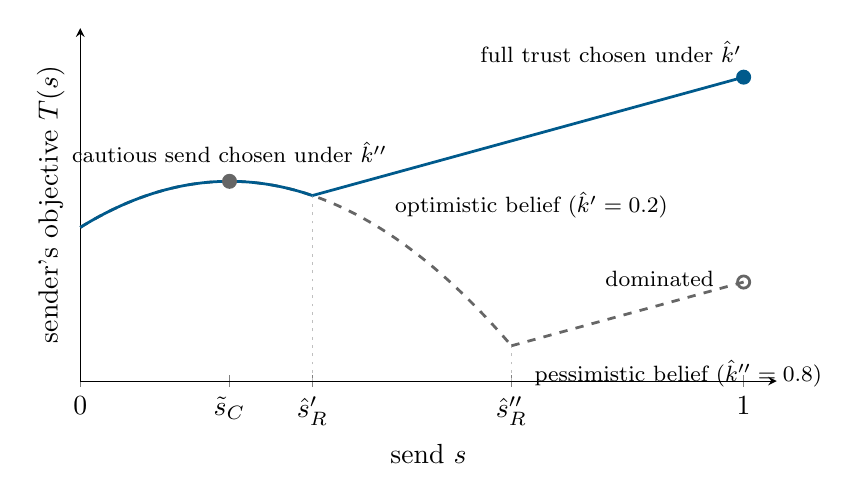
\begin{tikzpicture}
\begin{axis}[
    width=0.86\textwidth,
    height=0.5\textwidth,
    axis lines=left,
    xlabel={send $s$},
    ylabel={sender's objective $T(s)$},
    xmin=0, xmax=1.05,
    ymin=-0.55, ymax=2.55,
    xtick={0,0.225,0.35,0.65,1},
    xticklabels={$0$,$\tilde s_C$,$\hat s_R'$,$\hat s_R''$,$1$},
    ytick=\empty,
    tick style={black!50},
    every axis plot/.append style={line width=1pt},
    clip=false,
]
\addplot[black!25, dotted, line width=0.6pt] coordinates {(0.35,-0.55) (0.35,1.08)};
\addplot[black!25, dotted, line width=0.6pt] coordinates {(0.65,-0.55) (0.65,-0.24)};
\addplot[black!60, dashed, domain=0:0.65, samples=120] {(1-x)+0.3*(1+2*x)-0.5*(1-4*x)^2};
\addplot[black!60, dashed, domain=0.65:1, samples=2] {-1.28+1.6*x};
\addplot[csframe, domain=0:0.35, samples=80] {(1-x)+0.3*(1+2*x)-0.5*(1-4*x)^2};
\addplot[csframe, domain=0.35:1, samples=2] {0.52+1.6*x};
\addplot[only marks, mark=*, mark size=2.2pt, csframe] coordinates {(1,2.12)};
\addplot[only marks, mark=*, mark size=2.2pt, black!60] coordinates {(0.225,1.205)};
\addplot[only marks, mark=o, mark size=2.2pt, black!60] coordinates {(1,0.32)};
\node[anchor=south, font=\footnotesize] at (axis cs:0.80,2.16) {full trust chosen under $\hat k'$};
\node[anchor=north west, font=\footnotesize] at (axis cs:0.46,1.20) {optimistic belief ($\hat k'=0.2$)};
\node[anchor=south, font=\footnotesize] at (axis cs:0.225,1.28) {cautious send chosen under $\hat k''$};
\node[anchor=east, font=\footnotesize] at (axis cs:0.97,0.35) {dominated};
\node[anchor=north west, font=\footnotesize] at (axis cs:0.67,-0.28) {pessimistic belief ($\hat k''=0.8$)};
\end{axis}
\end{tikzpicture}
\caption{The sender's two plans.  The objective $T(s)$ at $m=3$, $\omega^S=(1,\,0.3,\,1)$, under an optimistic belief ($\hat k'=0.2$, solid) and a pessimistic belief ($\hat k''=0.8$, dashed).  The cautious branch is belief-independent, so the two curves coincide below the lower cutoff $\hat s_R'$.  Each curve is strictly concave on its cautious region, has a convex kink at its believed cutoff, and rises linearly on its trusting region.  Under the pessimistic belief the global optimum is the cautious send $\tilde s_C$ (filled circle; the corner $s=1$ is a dominated local optimum, open circle); under the optimistic belief it is full sending (filled circle).  For these preferences the belief threshold is $\bar k\approx0.56$.  No send at or near the believed cutoff, or strictly between the cutoff and one, is ever chosen.}
\label{fig:two_plans}
\end{figure}

Beliefs enter the sender's problem only through the believed return function.  Say that a belief $\hat\omega'$ is \emph{more pessimistic} than $\hat\omega$ if $\hat\omega'_o\ge\hat\omega_o$ and $\hat\omega'_d\le\hat\omega_d$: the believed receiver attends more to own earnings and less to the payoff gap, and by Proposition~\ref{prop:trust_return} returns weakly less at every send.  Lower believed returns can only hurt the sender: whenever the believed receiver returns anything he is, at his own optimum, still ahead of the sender, so an extra unit returned raises the sender's own payoff and reduces inequality at the same time.  Pessimism therefore lowers the value of every trusting plan, leaves every cautious plan untouched, and can only switch the sender from trusting to caution --- never the reverse.  The believed efficiency weight is irrelevant throughout, because the return choice reallocates a fixed total.  The next proposition records these claims; no assumptions beyond the setup are needed.  (And because the trusting send is pinned at $s=1$ by Lemma~\ref{lem:twobranch}, beliefs move only the \emph{decision} to trust, never the size of a trusting send.)

\begin{proposition}[Trust Sender: Monotone Belief Effects]
\label{prop:trust_beliefs}
Fix $\omega^S$ and let $\hat\omega'$ be more pessimistic than $\hat\omega$ (that is, $\hat\omega'_o\ge\hat\omega_o$ and $\hat\omega'_d\le\hat\omega_d$, with $\hat\omega'_e$ arbitrary).  Then:
\begin{enumerate}[topsep=2pt,itemsep=2pt]
\item \emph{(Values.)}  $\hat r(s;\hat\omega')\le\hat r(s;\hat\omega)$ and $T(s;\hat\omega')\le T(s;\hat\omega)$ for every $s$, with equality at every $s$ at which $\hat r(s;\hat\omega)=0$.  In particular the cautious candidate and its value are unchanged.
\item \emph{(Decision.)}  If under $\hat\omega$ every optimal send is cautious, then under $\hat\omega'$ every optimal send is cautious.  Equivalently, the willingness to trust is nonincreasing in $\hat\omega_o^{R}$, nondecreasing in $\hat\omega_d^{R}$, and independent of $\hat\omega_e^{R}$.
\item \emph{(Welfare.)}  The sender's maximal expected utility is nonincreasing in $\hat\omega_o^{R}$, nondecreasing in $\hat\omega_d^{R}$, and constant in $\hat\omega_e^{R}$.
\end{enumerate}
\end{proposition}

The sender's own weights affect both margins.  Within the cautious region the problem is a Dictator-like transfer problem scaled by the multiplier, and the cautious send responds to the weights accordingly.  The decision between the two plans is governed by the \emph{value of trusting},
\[
        G \;=\; \max_{[\hat s_R,1]}T \;-\; \max_{[0,\hat s_R]}T ,
\]
the gain from the best trusting plan over the best cautious plan: the sender trusts exactly when $G\ge0$.  Because utility is linear in the three attention weights, $G$ responds to each weight through the difference, between the two plans, of the payoff statistic that the weight multiplies: total payoff for $\omega_e^S$, own payoff for $\omega_o^S$, and the squared payoff gap for $\omega_d^S$.

\begin{proposition}[Trust Sender: Own-Weight Effects]
\label{prop:trust_ownweights}
\mbox{}
\begin{enumerate}[topsep=2pt,itemsep=2pt]
\item \emph{(Cautious send.)}  At an interior cautious optimum $s_C\in(0,\hat s_R)$,
\begin{csbox}
\[
        \frac{\partial s_C}{\partial \omega_o^S}<0,
        \qquad
        \frac{\partial s_C}{\partial \omega_e^S}>0,
        \qquad
        \sgn\frac{\partial s_C}{\partial \omega_d^S}
        =
        \sgn\big[1-(m+1)s_C\big],
\]
\end{csbox}
and $s_C$ is locally independent of beliefs.
\item \emph{(Trust decision.)}  $G$ is continuous in $\omega^S$ and, since the trusting candidate is full sending (Lemma~\ref{lem:twobranch}),
\begin{csbox}
\begin{gather*}
        \frac{\partial G}{\partial\omega_e^S}
        =(m-1)(1-s_C)>0,
        \qquad
        \frac{\partial G}{\partial\omega_o^S}
        =\Big(\frac m2-\hat k\Big)-(1-s_C),
        \\
        \frac{\partial G}{\partial\omega_d^S}
        =\frac{\big(1-(m+1)s_C\big)^2-4\hat k^2}{2}.
\end{gather*}
\end{csbox}
Hence: (i) efficiency attention \emph{always} favors trusting --- given $(\omega_o^S,\omega_d^S)$ and beliefs, there is a threshold $\bar\omega_e$ such that the sender trusts if and only if $\omega_e^S\ge\bar\omega_e$ (with the convention $\bar\omega_e=0$ or $+\infty$ when the decision does not switch); (ii) own-earnings attention favors trusting if and only if full sending delivers a higher believed own payoff than the best cautious send, $\tfrac m2-\hat k>1-s_C$; (iii) disparity attention favors trusting if and only if full sending delivers a more equal believed allocation than the best cautious send, $2\hat k<\big|1-(m+1)s_C\big|$.
\end{enumerate}
\end{proposition}

\noindent\emph{Intuition.}  In the cautious region, sending has a direct own-payoff cost of one unit per unit sent, an efficiency benefit because the amount sent is multiplied by $m>1$, and a disparity effect whose sign depends on which player is ahead: if the sender is ahead, sending reduces the payoff gap and disparity attention raises sending; if the receiver is already ahead, additional sending widens the gap and disparity attention lowers sending.  On the extensive margin, sending more always expands the believed pie; whether it also serves own earnings or equality depends on how much of the expanded pie the receiver is believed to hand back.  Efficiency attention is therefore the one motive that favors trusting unconditionally --- trusting is, in this model, fundamentally an efficiency phenomenon, disciplined by beliefs about the receiver.  Own-earnings and disparity attention favor trusting only conditionally, and the conditions are simple payoff comparisons between the two candidate plans.

\subsection{The Trust Decision: A Threshold in Believed Selfishness}

The two-candidate structure reduces the sender's problem to the comparison of two plans, and the believed receiver enters that comparison through the single scalar $\hat k$.  The decision to trust is therefore a threshold rule in believed selfishness.

\begin{proposition}[Trust Sender: Threshold Characterization]
\label{prop:trust_linear}
\mbox{}
\begin{enumerate}[topsep=2pt,itemsep=2pt]
\item If $\hat k\ge m/2$, the believed receiver never returns, the sender's objective is strictly concave on $[0,1]$, and $s_T^\ast=\min\{\max\{\tilde s_C,0\},1\}$.
\item If $\hat k<m/2$, the value gap
\[
        G(\hat k)
        =
        T(1)-T(s_C),
        \qquad
        T(1)=\omega_o^S\Big(\frac m2-\hat k\Big)+\omega_e^S m-2\omega_d^S\hat k^2,
\]
is continuous and strictly decreasing in $\hat k$, so there is a unique threshold $\bar k=\bar k(\omega^S,m)\le m/2$, possibly $-\infty$, such that
\[
        s_T^\ast=1\ \text{with positive believed return}
        \quad\Longleftrightarrow\quad
        \hat k\le\bar k .
\]
The threshold moves with the sender's weights according to $\sgn(\partial\bar k/\partial\theta)=\sgn(\partial G/\partial\theta)$, with the derivatives of Proposition~\ref{prop:trust_ownweights}(2); and $\partial G/\partial m>0$ throughout the no-trust region, so the trust region also expands with the multiplier.
\item If $\hat k>\bar k$, the sender is cautious and, necessarily, unconstrained by the cutoff: $s_T^\ast=\max\{0,\tilde s_C\}<\hat s_R$, with believed return zero.  In particular no sender ever chooses a send at, or just below, the believed cutoff: predicted sends are bimodal --- an interior cautious amount or everything.
\end{enumerate}
\end{proposition}

\begin{remark}[Where trust comes from]
Full trust hands the sender the believed share $\tfrac m2-\hat k$ of the multiplied pie, and the sender compares it with the cautious payoff.  In the purely selfish limit ($\omega_e^S\to0$, $\omega_d^S\to0$) the comparison collapses to own payoffs: $s_C=0$ and $G\ge0$ iff $\tfrac m2-\hat k\ge1$, i.e. $\bar k=\tfrac m2-1$.  A purely selfish sender fully trusts whenever the believed final-payoff gap conceded to the receiver, $2\hat k$, does not exceed $m-2$: for $m>2$ even a selfish sender trusts a believed-fair receiver, while for $m<2$ he never does.
\end{remark}

\noindent\emph{Intuition.}  Once returns are believed positive, the receiver raises the return at rate $(m+1)/2$, which keeps the believed payoff gap constant at $2\hat k$ as $s$ changes.  Disparity therefore no longer disciplines additional sending in the trusting region, while both own payoff and total surplus increase with the send: the best trusting plan is full sending.  The trust decision then reduces to a single comparison governed by one belief scalar, $\hat k$: optimism (low $\hat k$) means the sender expects nearly half of the multiplied pie back, and the threshold $\bar k$ rises with the motives that value the trusting outcome --- efficiency always, own earnings and equality when the believed receiver is fair enough --- and with the size of the pie itself.

Propositions~\ref{prop:trust_beliefs} and~\ref{prop:trust_linear} sign the \emph{decision} to trust; the analogue of Proposition~\ref{prop:ug_cs} would sign the chosen \emph{send} itself, globally.  Because the send jumps at the regime switch, global monotonicity requires the within-regime effect and the jump to point the same way.  This alignment holds for exactly two of the model's parameters: beliefs and the efficiency weight.

\begin{proposition}[Global Comparative Statics of the Trust Send]
\label{prop:trust_global}
The optimal send is globally monotone in beliefs and in the efficiency weight:
\begin{csbox}
\begin{gather*}
        s_T^\ast\ \text{is nonincreasing under belief pessimism and nondecreasing in }\omega_e^S\\
        \big(\text{nonincreasing in }\hat\omega_o^{R},\ \text{nondecreasing in }\hat\omega_d^{R},\ \text{constant in }\hat\omega_e^{R}\big).
\end{gather*}
\end{csbox}
In beliefs, the send is a step function: $s_T^\ast=1$ for $\hat k\le\bar k$, and the belief-independent cautious send $\max\{0,\tilde s_C\}$ above the threshold.  No such global statement holds for the remaining parameters: for $\omega_d^S$ and $m$ even the within-regime effect on the cautious send is not uniformly signed, and for $\omega_o^S$ the within-regime effects are uniformly nonpositive yet the extensive margin can flip the sign.
\end{proposition}

The failure in $\omega_o^S$ has, however, an exact structure.  Because the trusting candidate is pinned at full sending, the value of the trusting plan is \emph{linear} in the sender's weights, while the value of the cautious plan --- a maximum of functions linear in the weights --- is convex; the value of trusting $G$ is therefore concave in $\omega_o^S$, and concavity disciplines how greed can move the sender across regimes.

\begin{corollary}[Trust in Greed: An Interval]
\label{cor:greed_interval}
Suppose $\hat s_R\in(0,1)$, and fix $\omega_e^S$, $\omega_d^S$, and beliefs.
\begin{enumerate}[topsep=2pt,itemsep=2pt]
\item $G$ is concave in $\omega_o^S$, so the set of own-earnings weights at which the sender trusts is an interval (possibly empty): as greed rises, the sender switches regime at most twice --- into full trust, then back out.
\item As $\omega_o^S\to\infty$ the cautious send tends to zero and $\partial G/\partial\omega_o^S\to\big(\tfrac m2-\hat k\big)-1$: if $\hat k<\tfrac m2-1$, an arbitrarily greedy sender fully trusts; if $\hat k>\tfrac m2-1$, he sends nothing.
\end{enumerate}
\end{corollary}

\begin{remark}[Greed can increase sending]
The failure of global monotonicity in $\omega_o^S$ is a testable signature of the two-plan structure rather than a nuisance.  Within the cautious regime, own-earnings attention lowers the send; on the extensive margin, it favors trusting whenever full sending yields a higher believed own payoff than the best cautious send, $\tfrac m2-\hat k>1-s_C$ (Proposition~\ref{prop:trust_ownweights}).  This condition holds under optimistic beliefs, and intrinsic motives relax it further by raising the cautious send that trusting sacrifices: the phenomenon is easiest at large multipliers but is \emph{not} confined to $m>2$ --- at $m=2$, $\omega_e^S=0$, $\omega_d^S=1$, $\hat k=0.15$, the send falls from $\tfrac13$ within caution, jumps to $1$ near $\omega_o^S\approx0.27$, and drops back to caution near $\omega_o^S\approx3.0$.  By Corollary~\ref{cor:greed_interval} the pattern is nevertheless tightly disciplined: greed pushes the sender into full trust at most once, pushes him back out unless $\hat k\le\tfrac m2-1$, and the trust region in $\omega_o^S$ is always a single interval.  The model thus predicts that greed reduces sends among non-trusting senders yet can push senders across the trust threshold --- a pattern a monotone model cannot generate.
\end{remark}

\begin{remark}[Corner, step, and jump]
Two features of these results deserve emphasis.  First, within the trusting regime the send is pinned at the corner $s=1$, so every local comparative static of the sender's action is zero there: all sender-side comparative statics in that regime are \emph{threshold} statics --- how close the sender is to the regime boundary --- while the equilibrium outcome varies only through the receiver's response $r^\ast(1;\omega^R)$, which is interior and moves smoothly with the receiver's weights (Proposition~\ref{prop:trust_return}).  Second, the sender's action is discontinuous in his weights and beliefs --- smooth within the cautious regime, constant within the trusting regime, and jumping across the dominated middle region at the switch --- yet his value is continuous throughout: each branch value is a maximum of functions continuous in the parameters, and at the switch $G=0$ the sender is exactly indifferent between the two plans, so the jump discards no utility.  This is the generic signature of a bimodal objective.  Every other behavioral object in the paper solves a strictly concave problem and therefore varies continuously (the transfer, the minimum acceptable offer, the offer, the return); the convex kink of Lemma~\ref{lem:twobranch} is what makes the trust send the exception.
\end{remark}

\subsection{Trust Game Under Full Projection}

Under full projection in the Trust game the sender forecasts the trustee with his own weights, $\hat\omega^{R,T}=\omega^S$: the believed keep premium becomes the sender's own selfishness ratio over four, $\hat k=\kappa^S/4$, and the Trust prediction depends only on $(\omega^S,m)$.  Each own weight then operates through two channels: a preference channel (the weight enters the sender's objective directly) and a belief channel (the weight enters the projected receiver's return).  For the efficiency weight the belief channel is null, because the return choice does not depend on the receiver's efficiency weight (Proposition~\ref{prop:trust_return}); for the own-earnings and disparity weights the two channels resolve unambiguously.  Write $e^S=\omega_e^S/\omega_d^S$ for the efficiency ratio, alongside $\kappa^S$.

\begin{proposition}[Projected Trust Sender]
\label{prop:trust_projection}
Under full projection:
\begin{enumerate}[topsep=2pt,itemsep=2pt]
\item \emph{(Threshold.)}  There is a threshold $\bar\kappa(e^S,m)\in(0,2m]$, nondecreasing in $e^S$ and in $m$, such that the sender fully trusts ($s_T^\ast=1$ with positive believed return) if and only if $\kappa^S\le\bar\kappa(e^S,m)$; otherwise $s_T^\ast=\max\{0,\min\{\tilde s_C,1\}\}$ with believed return zero.
\item \emph{(Comparative statics: the decision to trust.)}  The full-trust indicator is globally monotone in every primitive:
\begin{csbox}
\[
        \text{full trust is}\quad
        \text{nonincreasing in }\omega_o^S,
        \qquad
        \text{nondecreasing in }\omega_e^S,\ \omega_d^S,\ \text{and }m.
\]
\end{csbox}
In particular the ambiguity of the own-earnings effect in Proposition~\ref{prop:trust_global} is resolved: under projection, greed both lowers the appetite for the trusting gamble and poisons the belief about the receiver, and the net effect is unambiguously against trusting.
\item \emph{(Comparative statics: the cautious send.)}  In the cautious regime ($\kappa^S>\bar\kappa$) with an interior send $s_T^\ast=\tilde s_C\in(0,\hat s_R)$, the belief channel is locally null and
\begin{csbox}
\[
        \frac{\partial s_T^\ast}{\partial \omega_o^S}<0,
        \qquad
        \frac{\partial s_T^\ast}{\partial \omega_e^S}>0,
        \qquad
        \sgn\frac{\partial s_T^\ast}{\partial \omega_d^S}
        =
        \sgn\big[1-(m+1)s_T^\ast\big].
\]
\end{csbox}
\item \emph{(Closed form.)}  In the region where the cautious candidate is interior and unconstrained, the trust condition $\kappa^S\le\bar\kappa(e^S,m)$ is the positivity region of the explicit concave quadratic
\[
        \tilde G(\kappa^S,e^S)
        =
        \frac{m(m-1)}{2(m+1)}\,\kappa^S
        +\frac{m(m-1)}{m+1}\,e^S
        -\frac38\,(\kappa^S)^2
        -\frac{\big(e^S(m-1)-\kappa^S\big)^2}{2(m+1)^2},
\]
and at $e^S=0$ the threshold is in closed form:
\[
        \bar\kappa(0,m)=\frac{4m(m-1)(m+1)}{3(m+1)^2+4}.
\]
\item \emph{(Global comparative statics: the send.)}  Combining the two margins, the optimal send itself is globally monotone in $\omega_o^S$ and $\omega_e^S$:
\begin{csbox}
\[
        s_T^\ast\ \text{is nonincreasing in }\omega_o^S
        \quad\text{and}\quad
        \text{nondecreasing in }\omega_e^S,
\]
\end{csbox}
while for $\omega_d^S$ and $m$ the effect on the cautious send is not uniformly signed and no global statement holds.
\end{enumerate}
\end{proposition}

\noindent\emph{Intuition.}  Projection turns the sender's belief into a mirror: a sender who attends to own earnings expects the receiver to do the same and keep a premium $2\hat k=\kappa^S/2$ of the multiplied pie.  Greed therefore cuts against trusting twice --- it raises the standard the trusting gamble must meet, and it worsens the projected terms of that gamble --- and the two channels never conflict.  Efficiency attention favors trusting twice over: it values the multiplied pie directly and, because the receiver's return choice does not change total surplus, projecting it onto the receiver costs nothing.  Disparity attention makes the sender expect equalizing returns and simultaneously makes the near-equal full-trust allocation attractive.  This is why, under projection, the Trust game delivers the cleanest possible sign pattern on the extensive margin: $(-,+,+)$ in the three own weights, $+$ in the multiplier.

\begin{remark}[Partial projection]
Partial projection, $\hat\omega^{R,T}=(1-\rho)\bar\omega+\rho\,\omega^S$, scales the belief channel by $\rho$ without changing its sign: greater $\omega_o^S$ still makes the projected belief more pessimistic and greater $\omega_d^S$ more optimistic, so by Proposition~\ref{prop:trust_beliefs} the belief channel of each own weight retains its full-projection direction for every $\rho>0$.  The efficiency-weight monotonicity holds verbatim for every $\rho\in[0,1]$, because the return choice never depends on the believed efficiency weight.  The unambiguous signs for $\omega_o^S$ and $\omega_d^S$ in Proposition~\ref{prop:trust_projection}, by contrast, do rely on full projection: for $\rho<1$ the preference channel can dominate at parameter values where it opposes the belief channel, so the clean monotonicity of the trust decision in those two weights is a genuine full-projection result.
\end{remark}

\clearpage

\section{The Trust Game with a Repayment Norm}
\label{sec:norm_repay}

This section presents, self-contained and in full, the Trust game in which fair conduct for the receiver is \emph{repayment}: give the sender back what he invested, and keep the surplus.

Recall the game.  The sender is endowed with one unit, the receiver with nothing.  The sender chooses how much to send, $s\in[0,1]$; the amount sent is multiplied by $m>1$; the receiver then chooses how much to return, $r\in[0,ms]$.  Material payoffs are
\[
        y_S=1-s+r,
        \qquad
        y_R=ms-r,
\]
and total payoff $q(s)=1+(m-1)s$ is fixed once the send is chosen: the send creates surplus, the return only divides it.  Players evaluate outcomes with the attention-weighted utility of Section~\ref{sec:setup}, attaching weight $\omega_o>0$ to own earnings, $\omega_e\ge0$ to total earnings, and $\omega_d>0$ to a disparity penalty.

What the receiver's disparity penalty targets is the departure from the gap-benchmark model of Section~\ref{sec:trust}.  A receiver who returns less than $s$ leaves the sender below his endowment: he has, in effect, kept part of what he was entrusted with.  A receiver who returns exactly $s$ makes the sender whole and keeps the entire multiplication surplus $(m-1)s$ for himself.  The \emph{repayment norm} takes this boundary as the standard of fair conduct --- debts are repaid, windfalls are kept --- and the receiver minds falling short of it:
\begin{equation}
\label{eq:norm2_utility}
        U^{R,T}
        =
        \omega_o^{R}(ms-r)
        +\omega_e^{R}\,q(s)
        -\frac{\omega_d^{R}}{2}\big(s-r\big)^{2}.
\end{equation}
Unlike the gap-benchmark receiver, who compares final earnings, this receiver compares his action to a reference action: he feels no obligation to share the multiplication surplus, only to give back the stake.  Everything else is as in the gap-benchmark model: the sender's disparity concern targets the final payoff gap, and the sender holds a point belief $\hat\omega^{R,T}$ about the receiver's weights.

\subsection{Receiver}

Fix a send $s>0$.  Returning is a pure transfer: each unit returned lowers the receiver's own earnings one for one and leaves total earnings $q(s)$ unchanged, so own-earnings attention pushes toward returning nothing and efficiency attention is silent about the return.  The one motive to return is the norm: at $r<s$ the receiver is short of full repayment by $s-r$, and the marginal relief from shrinking that debt, $\omega_d^{R}(s-r)$, is weighed against the constant marginal own-earnings cost $\omega_o^{R}$.

\begin{proposition}[Repayment Returns]
\label{prop:norm2_receiver}
For each $s\in[0,1]$ the receiver's return is unique:
\begin{csbox}
\[
        r^\ast(s;\omega^R)=\max\big\{0,\ s-c\big\},
        \qquad
        c=\frac{\omega_o^{R}}{\omega_d^{R}},
\]
\end{csbox}
where $c$ is the receiver's \emph{norm shortfall}.
\begin{enumerate}[topsep=2pt,itemsep=2pt]
\item \emph{(Cutoff and slope.)}  Returns are zero at or below the cutoff, which \emph{equals} the shortfall, $\bar s_I=c$ (interior exactly when $c<1$), and positive above it; positive returns are interior --- the receiver never fully repays --- and the marginal return is exactly one: past the cutoff, each additional unit sent is repaid in full.
\item \emph{(Comparative statics.)}  At an interior return,
\begin{csbox}
\[
        \frac{\partial r^\ast}{\partial \omega_o^{R}}<0,
        \qquad
        \frac{\partial r^\ast}{\partial \omega_e^{R}}=0,
        \qquad
        \frac{\partial r^\ast}{\partial \omega_d^{R}}>0.
\]
\end{csbox}
These signs hold globally as weak inequalities, with strictness exactly at an interior return; the cutoff is increasing in $\omega_o^{R}$, independent of $\omega_e^{R}$, and decreasing in $\omega_d^{R}$.
\end{enumerate}
\end{proposition}

\noindent\emph{Intuition.}  The receiver behaves like a debtor with a fixed temptation: he would like to pocket $c=\omega_o^{R}/\omega_d^{R}$ of the debt.  For small investments ($s\le c$) the temptation swallows the whole debt and nothing comes back; once $s$ exceeds $c$ he returns $s-c$, holding his shortfall from the norm constant --- so every marginal unit invested is repaid one for one.  More selfish receivers (higher $\omega_o^{R}$, lower $\omega_d^{R}$) have larger shortfalls: they return less at every investment and start returning later, and receivers with $c\ge1$ never return anything.  Contrast the gap-based receiver of Section~\ref{sec:trust}, who starts returning only once he is strictly ahead of the sender and then returns at marginal rate $\tfrac{m+1}2>1$: the repayment receiver is pinned to his conduct standard instead, and his returns can begin while the sender is still ahead.

\subsection{Sender}

The sender moves first and behaves as if the receiver's weights are $\hat\omega^{R,T}$ for sure.  The believed receiver is summarized by one number, the \emph{believed shortfall} $\hat c=\hat\omega_o^{R}/\hat\omega_d^{R}$: by Proposition~\ref{prop:norm2_receiver}, the sender expects the return $\hat r(s)=\max\{0,\,s-\hat c\}$, zero at or below the believed cutoff $\hat c$ and repaying each marginal unit in full above it.  Call $[0,\hat c]$ the \emph{cautious region} and $(\hat c,1]$ the \emph{trusting region}: a cautious sender expects nothing back, a trusting sender deliberately crosses the cutoff and relies on the believed repayment.  Assume $\hat c<1$, so that the believed cutoff is interior; otherwise the believed receiver never returns and the sender solves the strictly concave cautious problem below on all of $[0,1]$.

Substituting the believed return into the sender's utility gives believed payoffs $\hat y_S(s)=1-s+\hat r(s)$ and $\hat y_R(s)=ms-\hat r(s)$, believed gap $\hat d(s)=\hat y_S(s)-\hat y_R(s)$, and the objective
\begin{equation}
\label{eq:norm2_T}
        T(s)
        =
        \omega_o^S\,\hat y_S(s)
        +\omega_e^S\,q(s)
        -\frac{\omega_d^S}{2}\,\hat d(s)^2 .
\end{equation}
On the cautious region the sender expects nothing back, so his motives are intrinsic --- those of a dictator whose transfer is multiplied: sending costs one per unit, expands the pie by $m-1$ per unit, and moves the payoff gap $1-(m+1)s$.  The objective there is the belief-free strictly concave quadratic
\[
        T_0(s)=\omega_o^S(1-s)+\omega_e^S q(s)-\frac{\omega_d^S}{2}\big(1-(m+1)s\big)^2,
\]
with unconstrained maximizer
\[
        \tilde s_C
        =
        \frac{1}{m+1}
        +\frac{\omega_e^S(m-1)-\omega_o^S}{\omega_d^S(m+1)^2},
\]
and the \emph{cautious candidate} is the clipped version $s_C=\min\{\max\{\tilde s_C,0\},\hat c\}$.

On the trusting region the believed payoffs are
\[
        \hat y_S(s)=1-\hat c,
        \qquad
        \hat y_R(s)=(m-1)s+\hat c,
        \qquad
        \hat d(s)=1-2\hat c-(m-1)s .
\]
Because the believed receiver repays each marginal unit exactly, the sender's believed own payoff is \emph{flat} in the send: once he has decided to trust, he expects to end with his endowment less the shortfall $\hat c$, no matter how much he sends.  Trusting is believed to cost a fixed fee $\hat c$ --- the tribute to the receiver's temptation --- and, past that fee, the size of the send is a decision about \emph{other people's money}: each extra unit adds $m-1$ to the pie, all of it in the receiver's pocket.  Own-earnings attention is therefore indifferent about the size of a trusting send; efficiency attention pushes it up; and disparity attention pulls it back once the receiver moves ahead, since the believed gap falls at rate $m-1$.  The trusting branch is thus strictly concave, and it peaks where the believed gap equals $-\omega_e^S/\omega_d^S$: a sender without efficiency attention targets believed \emph{equality of final payoffs}, and efficiency attention pushes the target into the receiver's favor.  This is the central difference from the gap-benchmark model, where the believed gap is constant on the trusting region, the trusting branch is strictly increasing, and the only trusting candidate is full sending.

The sender's problem therefore reduces to comparing two plans: the best cautious send and the best trusting send.  Write $G$ for the \emph{value of trusting} --- the maximum of $T$ over the trusting region minus its maximum over the cautious region --- so that the sender trusts exactly when $G\ge0$.

\begin{lemma}[Two Concave Branches]
\label{lem:norm2_twobranch}
Let $\hat c<1$.  Then:
\begin{enumerate}[topsep=2pt,itemsep=2pt]
\item On the cautious region, $T=T_0$: strictly concave, with cautious candidate $s_C$.
\item On the trusting region, $T$ is a strictly concave quadratic with unconstrained maximizer
\[
        \tilde s_I=\frac{1-2\hat c+\omega_e^S/\omega_d^S}{m-1}.
\]
\item At $\hat c$ the marginal payoff jumps by $\omega_o^S-2\omega_d^S\big(1-(m+1)\hat c\big)$: writing $\kappa^S=\omega_o^S/\omega_d^S$, the kink is strictly convex if $\kappa^S>2\big(1-(m+1)\hat c\big)$ and strictly concave if the inequality is reversed --- in which case $T$ is strictly concave on all of $[0,1]$.
\item The cutoff itself is never optimal, and $s_T^\ast\in\{s_C,\,\min\{\tilde s_I,1\}\}$ whenever $\tilde s_I>\hat c$; otherwise every optimal send is cautious.
\end{enumerate}
\end{lemma}

Unlike in the gap-benchmark model, the kink need not be convex: a norm-based receiver can be believed to start returning while the sender is still ahead ($1-(m+1)\hat c>0$), where the onset of returns \emph{widens} the believed gap and hurts an inequality-averse sender.  When the kink is concave the whole problem is single-peaked and the policy continuous in weights and beliefs; otherwise the two-plan comparison and the jump in the policy survive.

\begin{proposition}[Equilibrium Behavior under the Repayment Norm]
\label{prop:norm2_sender}
Let $\hat c<1$.
\begin{enumerate}[topsep=2pt,itemsep=2pt]
\item \emph{(Equilibrium outcomes.)}  The optimal send is either the cautious candidate $s_C$ --- met, under correct beliefs, by zero return --- or the trusting send $\min\{\tilde s_I,1\}$, met by the positive return $s_T^\ast-c$.  On an open set of primitives the optimum is the \emph{interior} trusting send $s_T^\ast=\tilde s_I\in(\hat c,1)$, so under correct beliefs the model generates equilibrium outcomes in which both players' actions are interior.\footnote{For example, at $m=3$, $\omega^S=(1,\,0.5,\,1)$, $\hat c=0.3$: $s_T^\ast=0.45$ and the return is $0.15$.}
\item \emph{(Intensive margin.)}  At an interior trusting optimum,
\begin{csbox}
\begin{gather*}
        \frac{\partial s_T^\ast}{\partial\omega_o^S}=0,
        \qquad
        \frac{\partial s_T^\ast}{\partial\omega_e^S}=\frac{1}{(m-1)\omega_d^S}>0,
        \qquad
        \frac{\partial s_T^\ast}{\partial\omega_d^S}=-\frac{\omega_e^S}{(m-1)(\omega_d^S)^2}\le0,
        \\
        \frac{\partial s_T^\ast}{\partial\hat c}=-\frac{2}{m-1}<0,
        \qquad
        \frac{\partial s_T^\ast}{\partial m}=-\frac{\tilde s_I}{m-1}<0.
\end{gather*}
\end{csbox}
\item \emph{(Decision.)}  Wherever $G\le0$, the value of trusting is strictly decreasing in $\omega_o^S$ and $\hat c$ and strictly increasing in $\omega_e^S$, so the trust decision is characterized by a threshold in each parameter.  In particular greed is unambiguously against trusting: full repayment caps the trusting own payoff at $1-\hat c$, always below the cautious own payoff $1-s_C$.
\item \emph{(Global comparative statics.)}
\begin{csbox}
\begin{gather*}
        s_T^\ast\ \text{is globally nonincreasing in }\omega_o^S\ \text{and in }\hat c,\ \text{and globally nondecreasing in }\omega_e^S\\
        \big(\text{nonincreasing in }\hat\omega_o^{R},\ \text{nondecreasing in }\hat\omega_d^{R},\ \text{constant in }\hat\omega_e^{R}\big).
\end{gather*}
\end{csbox}
No global statement holds for $\omega_d^S$ or $m$.
\end{enumerate}
\end{proposition}

\noindent\emph{Intuition.}  Every comparative static flows from the flat believed own payoff.  Greed: own-earnings attention values the cautious plan at $1-s_C$ and any trusting plan at $1-\hat c<1-s_C$, so it lowers the cautious send, leaves the trusting send untouched, and votes against trusting --- sends fall in $\omega_o^S$ everywhere.  Efficiency: the trusting pie is larger and $\tilde s_I$ rises with $\omega_e^S$, so efficiency attention raises sends everywhere.  Pessimism: a higher believed shortfall $\hat c$ raises the fee to trusting, shrinks the trusting send, and leaves the cautious plan untouched, so sends fall.  Only disparity attention remains ambiguous, for the same reason as in the gap-benchmark model: whether sending narrows or widens the believed gap depends on which side of equality the sender starts from, and this is a fact about the sender's own motive, not about the receiver.

\begin{remark}[Greed monotonicity restored]
The gap-benchmark model's signature non-monotonicity --- greed can push senders across the trust threshold (Proposition~\ref{prop:trust_global}) --- disappears under the repayment norm.  The two receiver benchmarks are thereby separable in data: the gap benchmark predicts that greed pushes some favorably-believing senders into full trust, while the repayment norm predicts a uniformly negative relation between greed and sends.
\end{remark}

\subsection{The Repayment Norm Under Full Projection}

Under full projection the sender forecasts the receiver with his own weights, so the believed shortfall is the sender's own selfishness ratio, $\hat c=\kappa^S=\omega_o^S/\omega_d^S$, and the efficiency weight again has no belief channel (Proposition~\ref{prop:norm2_receiver}).  The trusting maximizer becomes
\[
        \tilde s_I=\frac{1-2\kappa^S+e^S}{m-1},
\]
and the one margin that was flat under free beliefs comes alive: greed does not change what a trusting sender expects to keep at the margin --- that is still exact repayment --- but it poisons his belief about the shortfall he must write off, so the trusting send now strictly falls in $\omega_o^S$.

\begin{proposition}[Projected Repayment Sender]
\label{prop:norm2_projection}
Under full projection:
\begin{enumerate}[topsep=2pt,itemsep=2pt]
\item \emph{(Regimes and threshold.)}  If $\kappa^S\ge1$, the projected receiver never returns, $T$ is strictly concave on $[0,1]$, and $s_T^\ast=\min\{\max\{\tilde s_C,0\},1\}$.  If $\kappa^S<1$, there is a threshold $\bar\kappa_I(e^S,m)$, nondecreasing in $e^S$, such that optimal sends are trusting if and only if $\kappa^S\le\bar\kappa_I$.
\item \emph{(Intensive margin.)}  At an interior trusting optimum,
\begin{csbox}
\[
        \frac{\partial s_T^\ast}{\partial\omega_o^S}=-\frac{2}{(m-1)\omega_d^S}<0,
        \qquad
        \frac{\partial s_T^\ast}{\partial\omega_e^S}=\frac{1}{(m-1)\omega_d^S}>0,
        \qquad
        \sgn\frac{\partial s_T^\ast}{\partial\omega_d^S}=\sgn\big[2\kappa^S-e^S\big].
\]
\end{csbox}
The greed effect is pure belief channel; interior trusting optima exist on an open set of primitives for every $m>1$.\footnote{For example, at $m=3$, $\omega^S=(0.3,\,0.5,\,1)$: $\kappa^S=0.3$, $s_T^\ast=\tilde s_I=0.45$, with believed return $0.15$.}
\item \emph{(Global comparative statics.)}
\begin{csbox}
\[
        \text{for every }m>1:\quad
        s_T^\ast\ \text{is globally nonincreasing in }\omega_o^S\ \text{and globally nondecreasing in }\omega_e^S.
\]
\end{csbox}
The free-belief greed monotonicity of Proposition~\ref{prop:norm2_sender} is reinforced: both channels now work against sending.  For $\omega_d^S$ and $m$ no global statement holds.
\end{enumerate}
\end{proposition}

% ================================================================
% SECTION TEMPORARILY DISABLED (state-dependent norm): delete the
% \iffalse ... \fi pair (and the matching pair around its proofs in
% the appendix) to restore it.
% ================================================================
\iffalse
\section{A State-Dependent Norm: Make the Trustor Whole, Then Equalize}
\label{sec:norm_compound}

The gap benchmark of Section~\ref{sec:trust} and the repayment norm of Section~\ref{sec:norm_repay} need not be exclusive.  Note first that the gap-benchmark receiver is himself norm-based: with $r_{eq}(s)\equiv\frac{(m+1)s-1}{2}$ the \emph{equalizing return}, the identity $y_S-y_R=2\big(r-r_{eq}(s)\big)$ turns the disparity term over final payoffs into a norm penalty $\frac{4\omega_d^{R}}{2}\big(r_{eq}(s)-r\big)^2$: a benchmark $\beta=r_{eq}$ with a rescaled weight, whose shortfall is exactly the keep premium of Proposition~\ref{prop:trust_return}.  Experimental returns typically track the repayment norm for small investments and payoff equality for large ones.  This section develops the benchmark with exactly that shape, the upper envelope
\begin{equation}
\label{eq:norm3_benchmark}
        \beta^\ast(s)=\max\big\{s,\ r_{eq}(s)\big\} :
\end{equation}
the smallest return that both makes the sender whole ($y_S\ge1$) and keeps him from ending up behind ($y_S\ge y_R$).  The two pieces cross at $s^\dagger=\frac1{m-1}$ --- one half at $m=3$ --- a location pinned by the payoff structure of the game, not by preferences.  We assume $m>2$ throughout this section: for $m\le2$ the crossing exits the unit interval, $\beta^\ast(s)=s$ on $[0,1]$, and Section~\ref{sec:norm_repay} applies unchanged.

\begin{proposition}[State-Dependent Return]
\label{prop:norm3_receiver}
For each $s\in[0,1]$ the receiver's return is unique:
\begin{csbox}
\[
        r^\ast(s;\omega^R)=\max\big\{0,\ \beta^\ast(s)-c\big\},
        \qquad
        c=\frac{\omega_o^{R}}{\omega_d^{R}},
\]
\end{csbox}
where $c$ is the receiver's norm shortfall.
\begin{enumerate}[topsep=2pt,itemsep=2pt]
\item \emph{(Cutoff and slopes.)}  Returns are zero at or below the cutoff --- $\bar s=c$ if $c<\frac1{m-1}$ and $\bar s=\frac{1+2c}{m+1}$ otherwise, interior exactly when $c<m/2$ --- and positive above it; positive returns are interior and never reach the benchmark.  The marginal return is $1$ below the crossing and $\frac{m+1}2$ above: at $m=3$, slope one up to half the endowment, slope two beyond, with the switch at fifty percent.
\item \emph{(Comparative statics.)}  At an interior return,
\begin{csbox}
\[
        \frac{\partial r^\ast}{\partial \omega_o^{R}}<0,
        \qquad
        \frac{\partial r^\ast}{\partial \omega_e^{R}}=0,
        \qquad
        \frac{\partial r^\ast}{\partial \omega_d^{R}}>0.
\]
\end{csbox}
These signs hold globally as weak inequalities, with strictness exactly at an interior return; the cutoff is increasing in $\omega_o^{R}$, independent of $\omega_e^{R}$, and decreasing in $\omega_d^{R}$.
\end{enumerate}
\end{proposition}

For the sender, let $\hat c=\hat\omega_o^{R}/\hat\omega_d^{R}$ and $\hat r(s)=\max\{0,\beta^\ast(s)-\hat c\}$.  Optimistic beliefs put the believed cutoff on the repayment segment; pessimistic beliefs wipe that segment out entirely and hand the problem back to the gap-benchmark model.

\begin{lemma}[Three Plans]
\label{lem:norm3_threeplan}
Let $m>2$ and $\hat c<m/2$.
\begin{enumerate}[topsep=2pt,itemsep=2pt]
\item If $\hat c\ge\frac1{m-1}$, then $\hat r(s)=\max\{0,\,r_{eq}(s)-\hat c\}$, the gap-benchmark believed return with keep premium $\hat k=\hat c$: the sender's problem coincides with that of Section~\ref{sec:trust}, and Lemma~\ref{lem:twobranch} and Propositions~\ref{prop:trust_linear}--\ref{prop:trust_global} apply verbatim.
\item If $\hat c<\frac1{m-1}$, $T$ has three branches: the cautious objective $T_0$ on $[0,\hat c]$; the strictly concave \emph{repayment branch} of Lemma~\ref{lem:norm2_twobranch} on $(\hat c,s^\dagger]$, with unconstrained maximizer $\tilde s_I=\frac{1-2\hat c+\omega_e^S/\omega_d^S}{m-1}$ and constant believed own payoff $\hat y_S\equiv1-\hat c$; and the affine \emph{equality branch} of the gap-benchmark model on $(s^\dagger,1]$, strictly increasing with slope $(m-1)\big(\omega_o^S/2+\omega_e^S\big)$ and constant believed gap $-2\hat c$.
\item The marginal payoff jumps by $\omega_o^S-2\omega_d^S\big(1-(m+1)\hat c\big)$ at $\hat c$ (either sign is possible) and by $\frac{m-1}{2}\big[\omega_o^S+4\omega_d^S\hat c\big]>0$ at $s^\dagger$: the upper kink is always convex, so the objective is never concave on $[0,1]$.
\item Neither kink is ever optimal, and $s_T^\ast\in\{s_C,\ \tilde s_I,\ 1\}$, where $s_C=\min\{\max\{\tilde s_C,0\},\hat c\}$ and $\tilde s_I$ is a candidate only when it lies in $(\hat c,s^\dagger)$.  No optimal send lies in $(s^\dagger,1)$.
\end{enumerate}
\end{lemma}

\begin{proposition}[State-Dependent Trust Sender]
\label{prop:norm3_sender}
Let $m>2$ and $\hat c<\frac1{m-1}$, and write $V_C$, $V_I$, $V_E$ for the values of the three plans: caution, interior repayment trust, and full trust.
\begin{enumerate}[topsep=2pt,itemsep=2pt]
\item \emph{(Predicted sends.)}  Optimal sends take at most three forms --- an intrinsic cautious amount below $\hat c$, an interior trusting send in $(\hat c,s^\dagger)$, or everything --- and never an amount strictly between $s^\dagger$ and $1$.  Each form is optimal on an open set of primitives, so under correct beliefs the model generates equilibrium outcomes with interior actions on both sides.\footnote{At $m=3$, $\omega^S=(0.05,\,0,\,1)$, $\hat c=0.2$: $s_T^\ast=\tilde s_I=0.3$, with believed return $0.1$ and believed final payoffs $(0.8,\,0.8)$ --- exactly equal.}
\item \emph{(Intensive margins.)}  The interior trusting send obeys the comparative statics of Proposition~\ref{prop:norm2_sender}(2) and targets the believed gap $\hat d(\tilde s_I)=-\omega_e^S/\omega_d^S$ --- near-equality when efficiency attention is small; the full-trust plan has believed return $\frac m2-\hat c$ and constant believed gap $2\hat c$ in the receiver's favor.
\item \emph{(Plan sorting.)}  By the envelope theorem,
\begin{csbox}
\[
        \frac{\partial(V_I-V_C)}{\partial\omega_o^S}=s_C-\hat c<0,
        \qquad
        \frac{\partial(V_E-V_I)}{\partial\omega_o^S}=\frac m2-1>0,
        \qquad
        \frac{\partial(V_E-V_I)}{\partial\omega_e^S}=m-q(\tilde s_I)>0 :
\]
\end{csbox}
own-earnings attention \emph{hollows out the middle}, pushing senders from interior trust down to caution or up to full trust; efficiency attention climbs the ladder from caution to interior trust to full trust; interior trust is the egalitarians' plan.
\item \emph{(Global comparative statics.)}  On the whole belief range $\hat c<m/2$,
\begin{csbox}
\begin{gather*}
        s_T^\ast\ \text{is nonincreasing in }\hat c\ \text{and nondecreasing in }\omega_e^S,\ \text{globally}\\
        \big(\text{nonincreasing in }\hat\omega_o^{R},\ \text{nondecreasing in }\hat\omega_d^{R},\ \text{constant in }\hat\omega_e^{R}\big).
\end{gather*}
\end{csbox}
The send is not globally monotone in $\omega_o^S$ or $\omega_d^S$: at $m=3$, $\omega_e^S=0$, $\omega_d^S=1$, $\hat c=0.2$, the send is the interior trusting $0.3$ for small $\omega_o^S$ and jumps to $1$ near $\omega_o^S\approx0.15$; at $\hat c=0.4$ it declines within caution and jumps to $1$ near $\omega_o^S\approx1.05$.
\end{enumerate}
\end{proposition}

\begin{remark}[Reading receiver and sender data]
On the receiver side the model \emph{is} the empirical pattern: returns track the repayment line for investments below half the endowment and the equality line above it, shifted down by the shortfall.  (A third natural benchmark, an equal split of the multiplied investment, $\beta=ms/2$, predicts returns along a line that observed returns never track; we do not pursue it.)  Two disciplined implications: the switch point is the parameter-free crossing $s^\dagger=\frac1{m-1}$ (fifty percent at $m=3$, where the slope doubles from one to two); and with heterogeneous shortfalls $c_i$ censored at zero returns, the gap between the mean return and the envelope equals $E[\min\{c_i,\beta^\ast(s)\}]$ --- increasing and concave in $s$, asymptoting at the mean shortfall --- while the fraction of zero returns falls with $s$ as $\Pr(c_i\ge\beta^\ast(s))$.  On the sender side, the sharp predictions are the hole --- no sends strictly between $s^\dagger$ and everything --- and the sorting of item 3: egalitarian senders (high $\omega_d^S$, e.g.\ generous Dictator behavior) choose interior trusting sends, efficiency-motivated senders send everything, and greed vacates the interior plan in both directions.
\end{remark}

\subsection{The State-Dependent Norm Under Full Projection}

Under full projection the believed shortfall is the sender's own selfishness ratio, $\hat c=\kappa^S$.  Projection turns out to \emph{close} the interior trusting margin that free beliefs open: the projected full-trust return, $\tfrac m2-\kappa^S$, is generous exactly when the sender's own greed --- and hence his projected shortfall --- is small, and for $m\ge3$ this makes full trust dominate the interior repayment plan wherever the latter exists.

\begin{proposition}[Projected State-Dependent Sender]
\label{prop:norm3_projection}
Under full projection with $m\ge3$:
\begin{enumerate}[topsep=2pt,itemsep=2pt]
\item \emph{(All-or-nothing is restored.)}  Whenever the interior repayment plan exists, full trust dominates it, so optimal sends are all-or-nothing, exactly as in the gap-benchmark model: $s_T^\ast\in\{\max\{0,\tilde s_C\},\,1\}$, and no send in $(\kappa^S,1)$ is ever optimal.\footnote{For $2<m<3$ the interior plan can survive projection: at $m=2.5$, $\omega^S=(0.29,\,0,\,1.19)$, the optimal send is $0.34$, strictly between $\kappa^S$ and $s^\dagger$ (verified directly).}
\item \emph{(Threshold and global comparative statics.)}  There is a threshold $\bar\kappa_\ast(e^S,m)$, nondecreasing in $e^S$, such that $s_T^\ast=1$ if and only if $\kappa^S\le\bar\kappa_\ast$, and
\begin{csbox}
\[
        s_T^\ast\ \text{is globally nonincreasing in }\omega_o^S\ \text{and globally nondecreasing in }\omega_e^S.
\]
\end{csbox}
For $\omega_d^S$ and $m$ no global statement holds.
\end{enumerate}
\end{proposition}

\begin{remark}[Beliefs are identified by the interior cluster]
At $m=3$ the two belief theories are separable in sender data: with free (for example, calibrated) beliefs the state-dependent model predicts a cluster of interior trusting sends strictly below fifty percent, a spike at one hundred percent, and a hole in between; under projection the interior cluster disappears and sends are bimodal --- small intrinsic amounts or everything.  The presence or absence of interior sends below the crossing thus speaks directly to how senders form beliefs.
\end{remark}
\fi
% ================== end of disabled section ==================



\section{Summary of Comparative Statics}
\label{sec:summary}

This section collects the model's comparative statics for the Dictator game, the Ultimatum game, and the two variants of the Trust game: the \emph{gap benchmark} of Section~\ref{sec:trust}, where the receiver's disparity penalty targets the final payoff gap $y_R-y_S$, and the \emph{repayment norm} of Section~\ref{sec:norm_repay}, where it targets the shortfall from returning the investment.  Table~\ref{tab:first_mover_point} reports local signs under free beliefs, Table~\ref{tab:first_mover_projection} under full projection, and Table~\ref{tab:trust_global_m3} compares the \emph{global} comparative statics of the trust send across the two variants.

\begin{table}[ht]
\centering
\small
\renewcommand{\arraystretch}{1.25}
\caption{Comparative statics under free beliefs}
\label{tab:first_mover_point}

\vspace{2pt}
\emph{Panel A: Second-mover behavior}\\[3pt]
\begin{tabular}{l ccc}
\toprule
Object & $\omega_o^R$ & $\omega_e^R$ & $\omega_d^R$ \\
\midrule
Ultimatum minimum acceptable offer $\tau^\ast$ & $-$ & $-$ & $+$ \\
Trust return $r^\ast$ (either benchmark) & $-$ & $0$ & $+$ \\
\bottomrule
\end{tabular}

\vspace{10pt}
\emph{Panel B: First-mover behavior}\\[3pt]
{\setlength{\tabcolsep}{4.5pt}%
\begin{tabular}{l ccc ccc}
\toprule
& \multicolumn{3}{c}{Own weights} &
\multicolumn{3}{c}{Believed receiver weights} \\
\cmidrule(lr){2-4}\cmidrule(lr){5-7}
Object
& $\omega_o^S$ & $\omega_e^S$ & $\omega_d^S$
& $\hat\omega_o^R$ & $\hat\omega_e^R$ & $\hat\omega_d^R$ \\
\midrule
Dictator transfer $s_D^\ast$
& $-$ & $0$ & $+$ & NA & NA & NA \\
Ultimatum offer $o^\ast$
& $-^{(a)}$ & $0$ & $+^{(a)}$ & $-^{(b)}$ & $-^{(b)}$ & $+^{(b)}$ \\
Trust cautious send $s_C$ (either benchmark)
& $-$ & $+$ & $\sgn[1-(m+1)s_C]$ & $0$ & $0$ & $0$ \\
Trusting decision --- gap benchmark
& $\pm^{(c)}$ & $+$ & $\pm^{(d)}$ & $-$ & $0$ & $+$ \\
Trusting decision --- repayment norm
& $-$ & $+$ & $\pm$ & $-$ & $0$ & $+$ \\
Interior trusting send $\tilde s_I$ --- repayment norm
& $0$ & $+$ & $-^{(e)}$ & $-$ & $0$ & $+$ \\
\bottomrule
\end{tabular}}

\vspace{5pt}
\parbox{0.94\textwidth}{\footnotesize
\emph{Notes.}  Signs are local effects at interior solutions; $0$ denotes a locally zero effect, NA a parameter that does not enter the problem, and $\pm$ a conditional sign.  \emph{Trust labels:} the \emph{cautious send} $s_C$ is the optimal send of a sender who expects no return --- the same belief-free problem in both variants (Lemmas~\ref{lem:twobranch} and~\ref{lem:norm2_twobranch}); the \emph{trusting decision} is whether the optimal send crosses the believed return cutoff; a trusting sender sends everything under the gap benchmark, while under the repayment norm his send is typically the \emph{interior trusting send} $\tilde s_I$.  The Panel A signs and the Dictator and Ultimatum-offer signs in Panel B also hold globally as weak inequalities (Propositions~\ref{prop:ug_mao}, \ref{prop:trust_return}, \ref{prop:norm2_receiver}, \ref{prop:dictator}, and~\ref{prop:ug_cs}); the two Trust benchmarks share the receiver signs but differ in the marginal return to the send, $\tfrac{m+1}2$ (gap) versus $1$ (repayment) in the positive-return region.  For the Ultimatum offer, $^{(a)}$ strict iff the offer is intrinsic ($\kappa^S<\Gamma(\hat\tau)$) and $^{(b)}$ strict iff the offer is strategic ($\kappa^S>\Gamma(\hat\tau)$ and $\hat\tau>0$).  Gap-benchmark decision (Propositions~\ref{prop:trust_beliefs} and~\ref{prop:trust_linear}): $^{(c)}$ positive iff full trust yields a higher believed own payoff than the cautious send, $\tfrac m2-\hat k>1-s_C$ (the trust region in $\omega_o^S$ is an interval, Corollary~\ref{cor:greed_interval}), and $^{(d)}$ positive iff full trust yields a more equal believed allocation.  Repayment rows: Proposition~\ref{prop:norm2_sender}; belief signs operate through the believed shortfall $\hat c=\hat\omega_o^{R}/\hat\omega_d^{R}$; $^{(e)}$ strict iff $\omega_e^S>0$.}
\end{table}

\begin{table}[ht]
\centering
\small
\renewcommand{\arraystretch}{1.25}
\caption{Comparative statics under full projection}
\label{tab:first_mover_projection}
\begin{tabular}{l ccc}
\toprule
Object & $\omega_o^S$ & $\omega_e^S$ & $\omega_d^S$ \\
\midrule
Dictator transfer $s_D^\ast$ & $-$ & $0$ & $+$ \\
Ultimatum offer $o^P$ & $-$ & $-^{(a)}$ & $+$ \\
Trust cautious send $s_C$ (either benchmark) & $-$ & $+$ & $\sgn[1-(m+1)s_C]$ \\
Full-trust decision --- gap benchmark & $-$ & $+$ & $+$ \\
Interior trusting send $\tilde s_I$ --- repayment norm & $-$ & $+$ & $\pm$ \\
\bottomrule
\end{tabular}

\vspace{5pt}
\parbox{0.94\textwidth}{\footnotesize
\emph{Notes.}  Projection ties the believed weights to the sender's own, so each sign combines the preference and belief channels.  The Dictator game involves no beliefs and is unchanged.  Ultimatum signs are for interior offers (Corollary~\ref{cor:ug_projection}); $^{(a)}$ strict exactly in the strategic regime, zero in the intrinsic regime.  Gap-benchmark rows: Proposition~\ref{prop:trust_projection}; the full-trust decision is also nondecreasing in the multiplier $m$.  Repayment row: Proposition~\ref{prop:norm2_projection}; the $\omega_d^S$ sign is $\sgn[2\kappa^S-e^S]$.  Combining margins, under projection the send is globally nonincreasing in $\omega_o^S$ and nondecreasing in $\omega_e^S$ in both Trust variants.}
\end{table}

\begin{table}[ht]
\centering
\small
\renewcommand{\arraystretch}{1.25}
\caption{Global comparative statics of the Trust send}
\label{tab:trust_global_m3}
\begin{tabular}{l cc cc}
\toprule
& \multicolumn{2}{c}{Free beliefs} & \multicolumn{2}{c}{Full projection} \\
\cmidrule(lr){2-3}\cmidrule(lr){4-5}
Parameter & Gap benchmark & Repayment norm & Gap benchmark & Repayment norm \\
\midrule
$\omega_o^S$ & NM$^{(a)}$ & $-$ & $-$ & $-$ \\
$\omega_e^S$ & $+$ & $+$ & $+$ & $+$ \\
$\omega_d^S$ & NM & NM & NM & NM \\
Belief pessimism & $-$ & $-$ & \multicolumn{2}{c}{(beliefs tied to own weights)} \\
Interior trusting send & never & open region & never & open region \\
\bottomrule
\end{tabular}

\vspace{4pt}
\parbox{0.94\textwidth}{\footnotesize
\emph{Notes.}  Entries are global weak signs of the optimal send $s_T^\ast$, for general $m>1$; NM = not globally monotone.  Gap benchmark: the receiver's disparity penalty targets the final payoff gap (Section~\ref{sec:trust}); repayment norm: it targets the shortfall from returning the investment (Section~\ref{sec:norm_repay}).  Belief pessimism: higher $\hat\omega_o^{R}$, lower $\hat\omega_d^{R}$.  $^{(a)}$ The failure has an exact structure: the trust region in $\omega_o^S$ is an interval, and extreme greed ends in full trust iff $\hat k<\tfrac m2-1$ (Corollary~\ref{cor:greed_interval}); the failure is exhibited for $m\ge2$.  Free-belief columns: Propositions~\ref{prop:trust_global} and~\ref{prop:norm2_sender}; projection columns: Propositions~\ref{prop:trust_projection} and~\ref{prop:norm2_projection}.  The last row records whether an equilibrium outcome with an interior send and an interior return exists (under correct beliefs in the free-belief columns; under projection, when the projected belief is correct): under the gap benchmark a trusting sender always sends everything, while under the repayment norm interior trusting sends arise on an open set of primitives.  Several entries extend to concave earnings utility --- the $\omega_e^S$ row in every column, the gap free-belief column, and the free-belief interior-trusting-send entries --- while the repayment $\omega_o^S$ sign is a linear-utility result (Appendix~\ref{sec:robust}).}
\end{table}

\clearpage
% (was \appendix) letter Part II's proofs section as II.A without resetting to Part I's scheme:
\setcounter{section}{0}
\renewcommand{\thesection}{II.\Alph{section}}
\section{Proofs}
\label{app:proofs_disparity}

\subsection*{Proof of Proposition~\ref{prop:dictator}}

$D$ is a strictly concave quadratic ($D_{ss}=-4\omega_d^S<0$) with $\Phi_D(s_D)=-\omega_o^S+2\omega_d^S(1-2s_D)$ strictly negative for $s_D\ge1/2$, so no maximizer lies weakly above $1/2$.  The unconstrained first-order condition solves to $\tfrac12-\tfrac{\kappa^S}4$, positive exactly when $\Phi_D(0)=2\omega_d^S-\omega_o^S>0$, i.e.\ $\kappa^S<2$; otherwise the maximum is the corner $s_D=0$.  The local comparative statics follow by differentiating the closed form.  The global weak versions follow because $\Phi_D$ is pointwise nonincreasing in $\omega_o^S$ and nondecreasing in $\omega_d^S$ on $[0,1/2)$, and a pointwise shift of the marginal payoff moves the maximizer of a strictly concave objective weakly in the same direction, including at the corner $s_D^\ast=0$; $\omega_e^S$ does not enter $\Phi_D$.
\qed

\subsection*{Proof of Proposition~\ref{prop:ug_mao}}

For $o<1/2$, $A_o(o;\omega^R)=\omega_o^R+2\omega_d^R(1-2o)>0$, and $A(1/2;\omega^R)=\omega_o^R/2+\omega_e^R>0$: on $[0,1/2]$ the acceptance value is strictly increasing and strictly positive by $o=1/2$, so it crosses zero at most once.  Since $A(0;\omega^R)=\omega_e^R-\omega_d^R/2$, the minimum acceptable offer is zero exactly when $\omega_e^R\ge\omega_d^R/2$.  Otherwise $A(\tau;\omega^R)=0$ is the quadratic $2\omega_d^R\tau^2-(\omega_o^R+2\omega_d^R)\tau+(\omega_d^R/2-\omega_e^R)=0$, whose discriminant simplifies to
\[
        (\omega_o^R+2\omega_d^R)^2-8\omega_d^R\Big(\frac{\omega_d^R}{2}-\omega_e^R\Big)
        =
        (\omega_o^R)^2+4\omega_o^R\omega_d^R+8\omega_d^R\omega_e^R=D>0;
\]
the quadratic is positive at $\tau=0$ and negative at $\tau=1/2$ (it equals $-\omega_o^R/2-\omega_e^R$ there), so its smaller root is the unique crossing in $(0,1/2)$, as displayed.

At an interior minimum acceptable offer, the implicit-function theorem applied to $A(\tau;\omega^R)=0$ gives
\[
        \frac{\partial \tau^\ast}{\partial \omega_o^R}
        =
        -\frac{\tau^\ast}{A_o(\tau^\ast;\omega^R)}<0,
        \qquad
        \frac{\partial \tau^\ast}{\partial \omega_e^R}
        =
        -\frac{1}{A_o(\tau^\ast;\omega^R)}<0,
        \qquad
        \frac{\partial \tau^\ast}{\partial \omega_d^R}
        =
        \frac{(1-2\tau^\ast)^2}{2A_o(\tau^\ast;\omega^R)}>0.
\]
For the global statement: $A(o;\omega^R)$ is pointwise nondecreasing in $\omega_o^R$ and $\omega_e^R$ and nonincreasing in $\omega_d^R$; since $A$ is strictly increasing on $[0,1/2]$ and $\tau^\ast$ is its unique crossing point (or the corner $0$), a pointwise upward shift of the acceptance value weakly lowers $\tau^\ast$ and a downward shift weakly raises it.
\qed

\subsection*{Proof of Proposition~\ref{prop:ug_offer}}

Offers below $\hat\tau$ are rejected and yield utility zero.  Offers at or above $\hat\tau$ (up to $1/2$) are accepted and yield
\[
        W(o;\omega^S)
        =
        \omega_o^S(1-o)
        +\omega_e^S
        -\frac{\omega_d^S}{2}(1-2o)^2,
\]
which is the same objective as \eqref{eq:D_objective} with $o$ in place of $s_D$.  By Proposition~\ref{prop:dictator}, $W$ is strictly concave and maximized at $s_D^\ast(\omega^S)\in[0,1/2]$.  Offers above $1/2$ are never optimal: if accepted they yield $W(o)<W(1/2)$ by strict concavity, and if rejected they yield $0<W(1/2)$, while the offer $1/2$ is always accepted since $A(1/2;\hat\omega^{R,U})>0$.  Since $\hat\tau\in[0,1/2]$, the best accepted offer is the maximizer of $W$ on $[\hat\tau,1/2]$, namely $\max\{s_D^\ast(\omega^S),\hat\tau\}$.  This accepted offer weakly dominates rejection: if the maximum is $s_D^\ast$, it is the best accepted offer; if the maximum is $\hat\tau$, then $\hat\tau\in[s_D^\ast,1/2]$ and concavity implies $W(\hat\tau)\ge W(1/2)>0$.

Dividing $\Phi_D(\hat\tau;\omega^S)$ by $\omega_d^S>0$ gives the factorization \eqref{eq:regime_factor}, so the sign of the marginal value $\Phi_D(\hat\tau;\omega^S)$ is the sign of $\Gamma(\hat\tau)-\kappa^S$.  Because $\Phi_D$ is strictly decreasing on $[0,1/2]$, if $\hat\tau>0$ we have $s_D^\ast>\hat\tau$ iff $\kappa^S<\Gamma(\hat\tau)$, $s_D^\ast<\hat\tau$ iff $\kappa^S>\Gamma(\hat\tau)$, and equality iff $\kappa^S=\Gamma(\hat\tau)$.  If $\kappa^S<\Gamma(\hat\tau)$ then also $\Phi_D(0;\omega^S)\ge\Phi_D(\hat\tau;\omega^S)>0$, so the Dictator optimum is interior and $o^\ast=s_D^\ast>0$.  If $\hat\tau=0$ and $\kappa^S>\Gamma(0)$, then $\Phi_D(0;\omega^S)<0$, so $s_D^\ast=0$ and $o^\ast=0$.  The index $\Gamma(\tau)=2(1-2\tau)$ is strictly decreasing on $[0,1/2]$.

For item 4: by Proposition~\ref{prop:ug_mao}, $\hat\tau=0$ iff $\hat\omega_e^{R}\ge\hat\omega_d^{R}/2$, in which case $\Gamma(\hat\tau)=\Gamma(0)=2$.  Otherwise $\hat\tau$ is the displayed root and
\[
        1-2\hat\tau=\frac{\sqrt{\hat D}-\hat\omega_o^{R}}{2\hat\omega_d^{R}},
        \qquad\text{so}\qquad
        \Gamma(\hat\tau)=\frac{\sqrt{\hat D}-\hat\omega_o^{R}}{\hat\omega_d^{R}}.
\]
Since $\sqrt{\hat D}\gtrless\hat\omega_o^{R}+2\hat\omega_d^{R}$ iff $\hat\omega_e^{R}\gtrless\hat\omega_d^{R}/2$, the two expressions combine into the stated minimum, attained by the first argument exactly in the believed-soft case.  The case list then instantiates items 1--3; in the believed-soft case $\Gamma(\hat\tau)=2$, and $\kappa^S\ge2$ merges the strategic corner ($\kappa^S>2$) with the kink at zero ($\kappa^S=2$), where the offer is zero either way.
\qed

\subsection*{Proof of Proposition~\ref{prop:ug_cs}}

The offer is the pointwise maximum of two continuous functions, hence continuous.  Each branch is monotone in each parameter with the direction claimed: $s_D^\ast$ is nonincreasing in $\omega_o^S$, nondecreasing in $\omega_d^S$, constant in $\omega_e^S$ and in beliefs (Proposition~\ref{prop:dictator}); $\hat\tau$ is nonincreasing in $\hat\omega_o^{R}$ and $\hat\omega_e^{R}$, nondecreasing in $\hat\omega_d^{R}$, constant in own weights (Proposition~\ref{prop:ug_mao}).  A pointwise maximum of functions that are all monotone in a given direction is monotone in that direction, including at the kink, where the one-sided derivatives are those of the two branches.  This proves global monotonicity; wherever a derivative of $o^\ast$ exists it therefore carries the stated weak sign, and at kink points both one-sided derivatives do.

Strictness: if $\kappa^S<\Gamma(\hat\tau)$ then $s_D^\ast>\hat\tau\ge0$ by Proposition~\ref{prop:ug_offer}, so the active branch is the interior Dictator transfer, which is strictly monotone in $\omega_o^S$ and $\omega_d^S$; the belief branch is inactive, so small belief changes do not move the offer.  If $\kappa^S>\Gamma(\hat\tau)$ and $\hat\tau>0$ the active branch is the interior believed minimum acceptable offer, which is strictly monotone in all three believed weights, while the own-weight branch is inactive.  At $\kappa^S=\Gamma(\hat\tau)$ the two branches coincide and one-sided derivatives apply.

Regime switching: the regime gap $\Gamma(\hat\tau)-\kappa^S$ is strictly decreasing in $\omega_o^S$ and strictly increasing in $\omega_d^S$, through $\kappa^S=\omega_o^S/\omega_d^S$ only, and constant in $\omega_e^S$.  Since $\Gamma$ is strictly decreasing, the gap inherits the opposite of the monotonicity of $\hat\tau$ in the believed weights (Proposition~\ref{prop:ug_mao}), which is strict whenever $\hat\tau$ is interior.  Monotonicity of the gap in each parameter implies the single-switch property, and the description of the paths follows by combining the branch formulas with the switch direction.
\qed

\subsection*{Proof of Corollary~\ref{cor:ug_projection}}

Under full projection $\hat\omega^{R,U}=\omega^S$, so the believed minimum acceptable offer in Proposition~\ref{prop:ug_offer} is $\tau^\ast(\omega^S)$, and the offer formula and regime characterization follow directly.  For the comparative statics: under projection both branches are monotone in the \emph{same} direction in $\omega_o^S$ and $\omega_d^S$ --- the Dictator transfer is strictly decreasing in $\omega_o^S$ and strictly increasing in $\omega_d^S$ whenever interior, and the projected minimum acceptable offer is strictly decreasing in $\omega_o^S$ and strictly increasing in $\omega_d^S$ whenever interior (Propositions~\ref{prop:dictator} and~\ref{prop:ug_mao}).  If $o^P>0$ the active branch (or, at the kink, both branches) is interior and strictly monotone, so the maximum is strictly monotone.  For $\omega_e^S$, the Dictator branch is constant and the projected acceptance branch is nonincreasing, so the maximum is nonincreasing, strictly when the acceptance branch is active and interior.
\qed

\subsection*{Proof of Proposition~\ref{prop:trust_return}}

The return objective is strictly concave in $r$ ($\Phi_{R,r}=-4\omega_d^R<0$), and $\Phi_R(ms,s;\omega^R)=-\omega_o^R+2\omega_d^R((1-m)s-1)<0$, so the upper corner never binds.  The first-order condition $-\omega_o^R+2\omega_d^R\big((m+1)s-1-2r\big)=0$ solves to the displayed closed form; the return is positive exactly when $s>\bar s_R=(1+2k)/(m+1)$, which is interior iff $k<m/2$, and at a positive return $g_R(r^\ast,s)=(m+1)s-1-2r^\ast=2k$, i.e.\ $y_R-y_S=2k$.  Differentiating the closed form gives the slope $(m+1)/2$ and the local comparative statics, and the cutoff statics follow from $\bar s_R=(1+2k)/(m+1)$.  For the global statement, evaluate $\Phi_R$ at the current optimum after the weight change: increasing $\omega_o^R$ lowers $\Phi_R$ pointwise, so by strict concavity the maximizer weakly falls and the corner $r^\ast=0$ persists; increasing $\omega_d^R$ raises $\Phi_R$ at an interior optimum (where $g_R=2k>0$) and at a corner with $g_R(0,s)\ge0$, so the maximizer weakly rises, while a corner with $g_R(0,s)<0$ has $\Phi_R(0,s)<0$ for all weights and persists; $\omega_e^R$ does not enter \eqref{eq:R_return_phi}.
\qed

\subsection*{Proof of Lemma~\ref{lem:twobranch}}

(1) On the cautious region $\hat r=0$, so
\[
        T(s)=T_0(s)\equiv\omega_o^S(1-s)+\omega_e^S\big(1+(m-1)s\big)-\frac{\omega_d^S}{2}\big(1-(m+1)s\big)^2,
\]
a quadratic with $T_0''=-\omega_d^S(m+1)^2<0$ and first-order condition $-\omega_o^S+\omega_e^S(m-1)+\omega_d^S(m+1)\big(1-(m+1)s\big)=0$, whose root is $\tilde s_C$; strict concavity makes the clipped candidate unique.

(2) At $s=\hat s_R$, $\hat r=0$ and $\hat d(\hat s_R)=1-(m+1)\hat s_R=-2\hat k<0$.  Subtracting the one-sided versions of \eqref{eq:T_sender_phi}, with $\hat r_s(\hat s_R^+)=\tfrac{m+1}2$,
\[
        T'_+(\hat s_R)-T'_-(\hat s_R)
        =
        \hat r_s(\hat s_R^+)\big[\omega_o^S-2\omega_d^S\hat d(\hat s_R)\big]
        =
        \frac{m+1}2\big[\omega_o^S+4\omega_d^S\hat k\big]>0.
\]

(3) For $s>\hat s_R$, $\hat r(s)=\frac{(m+1)s-1}{2}-\hat k$, so
\[
        \hat y_S(s)=\frac{1+(m-1)s}{2}-\hat k,
        \qquad
        \hat y_R(s)=\frac{1+(m-1)s}{2}+\hat k,
        \qquad
        \hat d(s)=-2\hat k,
\]
and substituting into \eqref{eq:T_sender_objective},
\[
        T(s)
        =
        \omega_o^S\left(\frac{1+(m-1)s}{2}-\hat k\right)
        +\omega_e^S\big(1+(m-1)s\big)
        -2\omega_d^S\hat k^2,
\]
affine and strictly increasing with slope $(m-1)\big(\omega_o^S/2+\omega_e^S\big)>0$; its unique maximizer on $[\hat s_R,1]$ is $s=1$, and the believed return and payoffs at $s=1$ follow by substitution.

(4) By (2)--(3), $T'_+(\hat s_R)>0$, so the cutoff is dominated by sends just above it and is never optimal; non-concavity on $[0,1]$ is immediate from (2) since concave functions have nonincreasing derivatives.  Combining (1) and (3), the global optimum is either the cautious candidate $s_C$ or full sending.
\qed

\subsection*{Proof of Proposition~\ref{prop:trust_beliefs}}

(1) \emph{Returns.}  The believed return $\hat r(s)=\max\{0,\tfrac{(m+1)s-1}2-\hat k\}$ is nonincreasing in $\hat k$, and pessimism raises $\hat k=\hat\omega_o^{R}/(4\hat\omega_d^{R})$, so $r^\ast(s;\hat\omega')\le r^\ast(s;\hat\omega)$ for every $s$.

\emph{Values.}  Fix $s$ with $r^\ast\equiv r^\ast(s;\hat\omega)>0$ and consider the sender's utility as a function of the return level $r$,
\[
        \psi(r)=\omega_o^S(1-s+r)+\omega_e^S q(s)-\frac{\omega_d^S}{2}\big(1-(m+1)s+2r\big)^2,
        \qquad
        \psi'(r)=\omega_o^S-2\omega_d^S\hat d(s,r),
\]
where $\hat d(s,r)=1-(m+1)s+2r$.  Receiver optimality gives $\hat d(s,r^\ast)=-2\hat k<0$, and $\hat d(s,\cdot)$ is increasing, so $\hat d(s,r)<0$ for all $r\le r^\ast$; hence $\psi'>0$ on $[0,r^\ast]$.  Since $\hat r(s;\hat\omega')\in[0,r^\ast]$, we get $T(s;\hat\omega')=\psi(\hat r(s;\hat\omega'))\le\psi(\hat r(s;\hat\omega))=T(s;\hat\omega)$.  Where $\hat r(s;\hat\omega)=0$ both returns are zero and the values coincide; in particular this holds on the cautious region, so the cautious candidate and its value are unaffected.

(2) Suppose every optimal send under $\hat\omega$ is cautious and let $s_0$ be one of them, so $T(s;\hat\omega)<T(s_0;\hat\omega)$ for every $s$ with $\hat r(s;\hat\omega)>0$.  Take any $s$ with $\hat r(s;\hat\omega')>0$.  By (1), $\hat r(s;\hat\omega)\ge\hat r(s;\hat\omega')>0$, hence
\[
        T(s;\hat\omega')\le T(s;\hat\omega)<T(s_0;\hat\omega)=T(s_0;\hat\omega'),
\]
the last equality because $\hat r(s_0;\hat\omega)=0$ implies $\hat r(s_0;\hat\omega')=0$.  So every trusting send is strictly suboptimal under $\hat\omega'$.

(3) Immediate from pointwise dominance.  Independence of $\hat\omega_e^{R}$: the believed return function does not depend on it, so neither does $T$.
\qed

\subsection*{Proof of Proposition~\ref{prop:trust_ownweights}}

(1) At an interior cautious optimum, $s_C=\tilde s_C$, and differentiating the closed form in Lemma~\ref{lem:twobranch}(1) gives
\[
        \frac{\partial s_C}{\partial\omega_o^S}=-\frac{1}{\omega_d^S(m+1)^2}<0,
        \qquad
        \frac{\partial s_C}{\partial\omega_e^S}=\frac{m-1}{\omega_d^S(m+1)^2}>0,
        \qquad
        \frac{\partial s_C}{\partial\omega_d^S}=\frac{\omega_o^S-\omega_e^S(m-1)}{(\omega_d^S)^2(m+1)^2},
\]
whose sign is that of $\omega_o^S-\omega_e^S(m-1)$, i.e.\ of $1-(m+1)s_C$ (from the first-order condition).  Beliefs enter $T$ only through $\hat r$, which is locally zero and locally invariant on the interior of the cautious region, so $s_C$ is locally independent of beliefs.

(2) Each branch value is a maximum of functions affine in $\omega^S$ over a compact set, hence convex and continuous in $\omega^S$.  By Lemma~\ref{lem:twobranch}(3) the trusting branch value is simply $T(1)$, affine in $\omega^S$ with coefficients $\big(\tfrac m2-\hat k,\,m,\,-2\hat k^2\big)$; the cautious branch value has the coefficients $\big(1-s_C,\,q(s_C),\,-\tfrac12(1-(m+1)s_C)^2\big)$ at its maximizer $s_C$, which is unique by Lemma~\ref{lem:twobranch}(1) (envelope theorem).  Subtracting gives the displayed derivatives.  For claim (i): $1>\hat s_R\ge s_C$, so $\partial G/\partial\omega_e^S=(m-1)(1-s_C)>0$.  Note also that wherever $G\le0$ the cautious candidate is interior to the cautious region: if $s_C=\hat s_R$, continuity of $T$ at the cutoff and the strict increase of $T$ beyond it (Lemma~\ref{lem:twobranch}(3)) imply $G>0$.  A continuous function of $\omega_e^S$ that is strictly increasing wherever it is nonpositive crosses zero at most once from below, which gives the threshold.
\qed

\subsection*{Proof of Proposition~\ref{prop:trust_linear}}

(1) If $\hat k\ge m/2$ then $\hat s_R\ge1$ and $\hat r\equiv0$ on $[0,1]$, so the sender's objective is the strictly concave cautious quadratic $T_0$ of Lemma~\ref{lem:twobranch}(1), and the optimum is the projection of $\tilde s_C$ on $[0,1]$.

(2) $T(1)$ is strictly decreasing in $\hat k$ (derivative $-\omega_o^S-4\omega_d^S\hat k<0$).  $T(s_C)$ is nondecreasing in $\hat k$: when $s_C<\hat s_R$ it is locally constant in $\hat k$, and when $s_C=\hat s_R$ it equals $T_0(\hat s_R)$ with $\hat s_R$ increasing in $\hat k$ and $T_0$ increasing on $[0,\tilde s_C]\supseteq[0,\hat s_R]$.  Hence $G$ is continuous and strictly decreasing in $\hat k$ and crosses zero at most once; set $\bar k=\sup\{\hat k\in[0,m/2):G(\hat k)\ge0\}$, with $\bar k=-\infty$ if the set is empty.  As $\hat k\to m/2$, $\hat s_R\to1$ and $T(1)\to T_0(1)\le T_0(s_C)$, so $G\le0$ in the limit and $\bar k\le m/2$.  Implicit differentiation of $G(\bar k)=0$, with $G_{\hat k}<0$, transfers the signs of Proposition~\ref{prop:trust_ownweights}(2) to $\bar k$.  For the multiplier: $\partial T(1)/\partial m=\omega_o^S/2+\omega_e^S$ (holding $\hat k$ fixed), and by the envelope theorem $\partial T_0(s_C)/\partial m=s_C\big[\omega_e^S+\omega_d^S(1-(m+1)s_C)\big]$.  If $s_C=0$ then $\partial G/\partial m=\omega_o^S/2+\omega_e^S>0$.  If $s_C=\tilde s_C$ is interior, the cautious first-order condition gives $\omega_d^S\big(1-(m+1)s_C\big)=\frac{\omega_o^S-\omega_e^S(m-1)}{m+1}$, so
\[
        \frac{\partial G}{\partial m}
        =
        \omega_o^S\Big(\frac12-\frac{s_C}{m+1}\Big)
        +\omega_e^S\Big(1-\frac{2s_C}{m+1}\Big)>0,
\]
using $s_C\le1<\tfrac{m+1}2$.  Since caution implies $s_C=\max\{0,\tilde s_C\}$ by item 3, this covers the whole no-trust region, so $G$ single-crosses zero from below in $m$.

(3) If the sender is cautious then $\tilde s_C<\hat s_R$: otherwise $s_C=\hat s_R$ and, since $T$ is continuous at $\hat s_R$ and strictly increasing beyond it, $T(1)>T(\hat s_R)=T(s_C)$, contradicting caution.  Hence $s_C=\max\{0,\tilde s_C\}$ strictly below the cutoff.
\qed

\subsection*{Proof of Proposition~\ref{prop:trust_global}}

Let $T_0$ be the belief-free cautious objective of Lemma~\ref{lem:twobranch}(1) and $\sigma_C=\min\{\max\{\tilde s_C,0\},1\}$ its maximizer on $[0,1]$.  Whenever the sender does not trust, his send is $\sigma_C$: if the trusting region is empty this is immediate; otherwise caution forces $s_C<\hat s_R$ (Proposition~\ref{prop:trust_linear}(3)), and then $s_C=\min\{\sigma_C,\hat s_R\}=\sigma_C$.  In particular the send under caution does not depend on beliefs.  Whenever the sender trusts, his send is $1$ (Lemma~\ref{lem:twobranch}(3)).  So for every belief,
\[
        s_T^\ast\in\{\sigma_C,\,1\},
        \qquad
        \sigma_C\le1,
\]
with $s_T^\ast=1$ exactly when the sender trusts, i.e.\ when $\hat k\le\bar k$ (Proposition~\ref{prop:trust_linear}).

\emph{Beliefs.}  Fix $\omega^S$ and make the belief more pessimistic ($\hat\omega_o^{R}$ weakly up, $\hat\omega_d^{R}$ weakly down, $\hat\omega_e^{R}$ arbitrary).  By Proposition~\ref{prop:trust_beliefs}(2) the trust decision can only switch from trusting to caution, so the send moves (if at all) from $1$ down to $\sigma_C$: it is nonincreasing.  Coordinate-wise monotonicity in $\hat\omega_o^{R}$ and $\hat\omega_d^{R}$, and constancy in $\hat\omega_e^{R}$, are special cases, and the step function is as displayed.

\emph{Efficiency.}  Within the cautious regime $s_T^\ast=\sigma_C$ is nondecreasing in $\omega_e^S$: $\partial\Phi_T/\partial\omega_e^S=m-1>0$ pointwise, and a pointwise upward shift of the marginal payoff moves the maximizer of the strictly concave $T_0$ weakly up, including at the corners.  Within the trust regime $s_T^\ast=1$ is constant.  By Proposition~\ref{prop:trust_ownweights}(2), $G$ is continuous and strictly increasing in $\omega_e^S$ wherever $G\le0$, so as $\omega_e^S$ increases the regime switches at most once, from caution to trust; at the switch the send jumps from $\sigma_C<\hat s_R<1$ up to $1$.  A function that is nondecreasing within regimes and jumps upward at its unique switch is globally nondecreasing.

\emph{Failure for the remaining parameters.}  For $\omega_d^S$ and $m$ the within-regime effect on the cautious send is not uniformly signed (Proposition~\ref{prop:trust_ownweights}(1)).  For $\omega_o^S$, take $\omega_e^S=0$, $\omega_d^S=1$, $m>2$, and $0<\hat k<\tfrac m2-1$.  As $\omega_o^S\downarrow0$, $G\to-2\hat k^2<0$, so the sender is cautious with send near $1/(m+1)$, decreasing in $\omega_o^S$.  For $\omega_o^S\ge m+1$ the cautious candidate is $s_C=0$ and $G=\omega_o^S\big(\tfrac m2-\hat k-1\big)+\tfrac12-2\hat k^2$, which is strictly increasing and eventually positive, so the sender eventually trusts fully.  The send therefore falls with $\omega_o^S$ over the cautious range and then jumps to $1$: it is not globally monotone.
\qed

\subsection*{Proof of Corollary~\ref{cor:greed_interval}}

(1) By Lemma~\ref{lem:twobranch}(3) the trusting value is $V_T=T(1)=\omega_o^S(\tfrac m2-\hat k)+\omega_e^S m-2\omega_d^S\hat k^2$, linear in $\omega_o^S$, while the cautious value $V_C=\max_{s\in[0,\hat s_R]}T(s)$ is a maximum of functions linear in $\omega_o^S$, hence convex.  Thus $G=V_T-V_C$ is concave in $\omega_o^S$, its superlevel set $\{G\ge0\}$ is an interval, and the regime switches at most twice as $\omega_o^S$ increases: into trust, then out.

(2) By the envelope theorem, at points of differentiability $\partial G/\partial\omega_o^S=(\tfrac m2-\hat k)-(1-s_C)$.  As $\omega_o^S\to\infty$, $\tilde s_C\to-\infty$, so $s_C\to0$ and $\partial G/\partial\omega_o^S\to(\tfrac m2-\hat k)-1$.  If $\hat k<\tfrac m2-1$ this limit is positive and $G\to+\infty$: the sender trusts for all large $\omega_o^S$.  If $\hat k>\tfrac m2-1$ it is negative and $G\to-\infty$: the sender is cautious for all large $\omega_o^S$, with send $s_C\to0$.
\qed

\subsection*{Proof of Proposition~\ref{prop:trust_projection}}

By homogeneity of degree one of utility in the weight vector (and degree zero of $\hat k$, $\hat s_R$, and $\tilde s_C$), the trust decision depends only on $(\kappa^S,e^S,m)$; normalize $\omega_d^S=1$, so $\hat k=\kappa^S/4$ and $\hat s_R=\frac{1+\kappa^S/2}{m+1}$.  Write $H=\{(\kappa^S,e^S):\kappa^S>0,\ e^S\ge0,\ e^S(m-1)\le \kappa^S\tfrac{m+3}2\}$ for the set on which the cautious candidate is not constrained by the cutoff (the inequality is $\tilde s_C\le\hat s_R$, rearranged).

\emph{Off $H$ the sender trusts.}  If $\tilde s_C>\hat s_R$ then $s_C=\hat s_R$ and, exactly as in the proof of Proposition~\ref{prop:trust_linear}(3), continuity of $T$ at the cutoff and strict increase beyond it give $T(1)>T(s_C)$, so $G>0$.

\emph{On $H$, $G$ is concave in $(\kappa^S,e^S)$ jointly.}  On $H$ the cautious value equals the unconstrained value $V_C(\kappa^S,e^S)=\max_{s\in[0,1]}T_0(s;\kappa^S,e^S)$, a maximum of functions affine in $(\kappa^S,e^S)$, hence convex; and $T(1)=\tfrac m2\kappa^S-\tfrac38(\kappa^S)^2+e^Sm$ is a concave quadratic (substituting $\hat k=\kappa^S/4$).  So $G=T(1)-V_C$ is concave on the convex set $H$, continuous, with $G(0,0)=0$.

\emph{Threshold in $\kappa^S$ and monotonicity in $e^S$.}  On $H$, $\partial G/\partial e^S=(m-1)(1-s_C)>0$ wherever $s_C<1$, which holds throughout the no-trust region.  Fix $e^S$ and increase $\kappa^S$: the set of $\kappa^S$ with $(\kappa^S,e^S)\in H$ is a half-line $\{\kappa^S\ge \kappa_a(e^S)\}$, $G$ is concave along it, and $G>0$ at its left endpoint --- either $\kappa_a(e^S)>0$, which lies on the boundary of $H$ where $\tilde s_C=\hat s_R$ and the trusting candidate strictly dominates by the first step, or $\kappa_a(e^S)=0$ (the case $e^S=0$), where $G\to0$ as $\kappa^S\downarrow0$ with strictly positive right derivative $\frac{m(m-1)}{2(m+1)}$.  A concave function positive at the left endpoint of a half-line is nonnegative exactly on an interval attached to that endpoint; joined with the all-trust region off $H$, the trust region at fixed $e^S$ is an interval $[0,\bar\kappa(e^S,m)]$ with $\bar\kappa>0$.  That $\bar\kappa$ is nondecreasing in $e^S$ follows from $\partial G/\partial e^S>0$ on $H$ together with the fact that the complement of $H$ is an upper set in $e^S$ at fixed $\kappa^S$.  That $\bar\kappa\le2m$ follows because $\kappa^S\ge2m$ means $\hat k\ge m/2$ and full trust is infeasible; indeed as $\kappa^S\to2m$, $T(1)\to T_0(1)\le V_C$, so $G\le0$ there.

\emph{Monotonicity in the raw weights.}  Increasing $\omega_o^S$ raises $\kappa^S$ leaving $e^S$ fixed, so the trust indicator can only switch from 1 to 0.  Increasing $\omega_e^S$ raises $e^S$ leaving $\kappa^S$ fixed, so by the previous paragraph the indicator can only switch from 0 to 1.  Increasing $\omega_d^S$ scales $(\kappa^S,e^S)$ toward the origin along a ray.  Rays through the origin either lie entirely in $H$ or entirely outside it, because the constraint defining $H$ is homogeneous.  Outside $H$, trust always holds.  Inside, $t\mapsto G(t\kappa_0,te_0)$ is concave with value $0$ at $t=0$ and strictly positive right derivative $\frac{m(m-1)}{2(m+1)}\kappa_0+\frac{m(m-1)}{m+1}e_0>0$, so $\{t\ge0:G\ge0\}$ is an interval $[0,\bar t]$; lowering $t$ (raising $\omega_d^S$) can only switch the indicator from 0 to 1.

\emph{Monotonicity in $m$.}  Under projection $\hat k$ does not depend on $m$, so the computation in the proof of Proposition~\ref{prop:trust_linear}(4) applies verbatim: $\partial G/\partial m>0$ throughout the no-trust region, giving single crossing.

\emph{Item 3.}  In the cautious regime $G<0$ strictly, so small parameter changes keep the sender cautious, and $\tilde s_C<\hat s_R$: a cautious candidate clipped at the cutoff would be strictly dominated by full trust, as shown in the first step.  On a neighborhood of $\tilde s_C$ the believed return is identically zero, and it remains so after small changes in $\omega^S$ because the projected cutoff $\hat s_R=\frac{1+\kappa^S/2}{m+1}$ moves continuously.  Only the preference channel therefore operates locally, and the signs follow by differentiating the closed form of $\tilde s_C$, as in Proposition~\ref{prop:trust_ownweights}(1).

\emph{Item 4.}  When $0\le\tilde s_C\le\hat s_R$, the vertex value of the cautious quadratic is
\[
        T_0(\tilde s_C)=\frac{m}{m+1}\kappa^S+\frac{2m}{m+1}e^S+\frac{\big(e^S(m-1)-\kappa^S\big)^2}{2(m+1)^2},
\]
and subtracting from $T(1)$ gives $\tilde G$.  At $e^S=0$,
\[
        \tilde G(\kappa^S,0)=\kappa^S\left[\frac{m(m-1)}{2(m+1)}-\left(\frac38+\frac1{2(m+1)^2}\right)\kappa^S\right],
\]
whose positive root is the displayed $\bar\kappa(0,m)$.

\emph{Item 5.}  Within the trust regime the send is constant at $1$; within the cautious regime it equals $\max\{0,\tilde s_C\}$, decreasing in $\omega_o^S$ and increasing in $\omega_e^S$; and by item 2 each of these parameters switches the regime at most once --- from trust to cautious as $\omega_o^S$ increases, with the send dropping from $1$ to $\max\{0,\tilde s_C\}<\hat s_R<1$, and from cautious to trust as $\omega_e^S$ increases, with the send jumping up to $1$.  Monotone within regimes with a single like-signed jump implies global monotonicity.  For $\omega_d^S$ and $m$ the cautious-send effect is not uniformly signed (item 3), so no global sign is possible.
\qed

\subsection*{Proof of Proposition~\ref{prop:norm2_receiver}}

The return objective is strictly concave in $r$, with marginal value $\Phi(r,s)=-\omega_o^{R}+\omega_d^{R}(s-r)$ and $\partial\Phi/\partial r=-\omega_d^{R}<0$; at $r=s$, $\Phi=-\omega_o^{R}<0$, so $r^\ast<s\le ms$: the receiver never fully repays and the upper corner never binds.  The first-order condition solves to the displayed closed form $r^\ast=\max\{0,s-c\}$: the return is positive exactly above the cutoff $\bar s_I=c$, interior exactly when $c<1$, and the marginal return is one.  Differentiating the closed form gives the local comparative statics and the cutoff statics.  The global weak versions follow because $\Phi$ is pointwise decreasing in $\omega_o^{R}$, increasing in $\omega_d^{R}$ at any optimum with $s-r\ge0$ (the corner at $s=0$ persists), and free of $\omega_e^{R}$, and a pointwise shift of a strictly concave objective's marginal value moves the maximizer weakly in the same direction.
\qed

\subsection*{Proof of Lemma~\ref{lem:norm2_twobranch}}

(1) On the cautious region $\hat r=0$, so $T=T_0$, the belief-free cautious objective displayed in the text, strictly concave with unconstrained maximizer $\tilde s_C$ (Lemma~\ref{lem:twobranch}(1)).

(2) For $s>\hat c$, $\hat r(s)=s-\hat c$ gives the believed payoffs displayed in the text; substituting into \eqref{eq:norm2_T},
\[
        T(s)=\omega_o^S(1-\hat c)+\omega_e^S\big(1+(m-1)s\big)-\frac{\omega_d^S}{2}\big(1-2\hat c-(m-1)s\big)^2,
\]
a quadratic with $T''=-\omega_d^S(m-1)^2<0$ and maximizer $\tilde s_I$.

(3) As in the proof of Lemma~\ref{lem:twobranch}(2), the one-sided derivatives at the cutoff differ by $\hat r_s(\hat c^+)\big[\omega_o^S-2\omega_d^S\hat d(\hat c)\big]=\omega_o^S-2\omega_d^S\big(1-(m+1)\hat c\big)$ --- but $\hat d(\hat c)=1-(m+1)\hat c$ is no longer signed, because the norm-based cutoff condition does not force the receiver ahead of the sender.  When the jump is negative, $T'$ is decreasing on each branch and falls at the kink, so $T$ is strictly concave on $[0,1]$.

(4) A convex kink cannot be a local maximum, by the argument in the proof of Lemma~\ref{lem:twobranch}(4).  If the kink is concave then $d_0\equiv1-(m+1)\hat c>0$ and $T'_+(\hat c)=(m-1)\big[\omega_e^S+\omega_d^S d_0\big]>0$, so the cutoff is dominated from the right in the concave case too.  By strict concavity of each branch, the maximum over the cautious region is $s_C$ and the maximum over the trusting region is $\min\{\tilde s_I,1\}$ when $\tilde s_I>\hat c$; when $\tilde s_I\le\hat c$ the trusting branch is nonincreasing, its supremum is the cutoff value $T_0(\hat c)\le T_0(s_C)$, and every optimal send is cautious.
\qed

\subsection*{Proof of Proposition~\ref{prop:norm2_sender}}

(1) The two-candidate structure is Lemma~\ref{lem:norm2_twobranch}(4), and under correct beliefs the return met by each candidate is given by Proposition~\ref{prop:norm2_receiver}: zero at $s_C\le\hat c=\bar s_I$, and $s_T^\ast-c\in(0,ms_T^\ast)$ at a trusting send.  For openness: at $m=3$, $\omega^S=(1,0.5,1)$, $\hat c=0.3$: $\tilde s_I=0.45\in(0.3,1)$, $s_C=\tilde s_C=1/4$, and $G=1.525-1.5>0$; all quantities are continuous in $(\omega^S,\hat c,m)$ and all inequalities strict, so the configuration survives on an open neighborhood, and the equilibrium return is $s_T^\ast-c=0.15$.

(2) Differentiate $\tilde s_I$.

(3) Wherever $G\le0$ the cautious candidate is unclipped, $s_C=\max\{0,\tilde s_C\}<\hat c$: if $s_C=\hat c$ then $T_0'(\hat c)\ge0$, and since the cutoff is dominated from the right (Lemma~\ref{lem:norm2_twobranch}(3)--(4)), $T$ strictly increases past it and $G>0$, a contradiction.  \emph{Own weight:} on the whole trusting branch $\hat y_S\equiv1-\hat c$, including at the clipped cutoff where $\hat r=0$, so by the envelope theorem $\partial G/\partial\omega_o^S=(1-\hat c)-(1-s_C)=s_C-\hat c<0$.  \emph{Efficiency:} $\partial G/\partial\omega_e^S=q(s_+)-q(s_C)>0$ as before.  \emph{Beliefs:} at an interior trusting optimum the first-order condition gives $\hat d(\tilde s_I)=-\omega_e^S/\omega_d^S\le0$, so $\partial T(\tilde s_I)/\partial\hat c=-\omega_o^S+2\omega_d^S\hat d(\tilde s_I)=-\omega_o^S-2\omega_e^S<0$; in the clipped case $\partial T_0(\hat c)/\partial\hat c=T_0'(\hat c)<0$; and at the corner $s_+=1$, $\partial T(1)/\partial\hat c=-\omega_o^S+2\omega_d^S\big(2-m-2\hat c\big)$, which is negative unless $2-m-2\hat c>\kappa^S/2>0$ --- a case incompatible with $G\le0$, because $\hat c<\tfrac{2-m}2-\tfrac{\kappa^S}4$ implies
\[
        \tilde s_C-\hat c
        \ \ge\ \frac1{m+1}-\frac{\kappa^S}{(m+1)^2}-\hat c
        \ >\ \frac{m(m-1)}{2(m+1)}+\frac{\kappa^S(m-1)(m+3)}{4(m+1)^2}
        \ >\ 0 ,
\]
so the cautious candidate would be clipped at the cutoff and the sender would trust.  Hence $G$ is strictly decreasing in $\omega_o^S$ and $\hat c$ and strictly increasing in $\omega_e^S$ wherever $G\le0$, which yields the thresholds.

(4) Within the cautious regime the send $\max\{0,\tilde s_C\}$ falls in $\omega_o^S$, rises in $\omega_e^S$, and is constant in $\hat c$; within the trust regime it is $\min\{\tilde s_I,1\}$, constant in $\omega_o^S$, nondecreasing in $\omega_e^S$, and nonincreasing in $\hat c$.  By item 4 each of the three parameters switches the regime at most once --- out of trust as $\omega_o^S$ or $\hat c$ rises, into trust as $\omega_e^S$ rises --- and at the switch the send jumps in the like direction, between a cautious send below $\hat c$ and a trusting send strictly above it.  Monotone within regimes with a single like-signed jump implies global monotonicity.  For $\omega_d^S$ the cautious send strictly rises when $s_C<1/(m+1)$ while the trusting send strictly falls when $\omega_e^S>0$; for $m$ the trusting send strictly falls while the cautious send can strictly rise (e.g.\ $\omega_o^S=0$, $\omega_e^S/\omega_d^S$ large, $m<3$); so no global statement holds for either.
\qed

\subsection*{Proof of Proposition~\ref{prop:norm2_projection}}

(1) If $\kappa^S\ge1$ the believed cutoff $\hat c=\kappa^S$ leaves the unit interval, $\hat r\equiv0$, and $T=T_0$.  For $\kappa^S<1$ the threshold follows from item 3: wherever $G\le0$, $G$ is strictly decreasing in $\omega_o^S$ (hence in $\kappa^S$ at fixed $\omega_d^S$) and strictly increasing in $\omega_e^S$, so each parameter crosses the trust boundary at most once.

(2) Substitute $\hat c=\kappa^S$ into Lemma~\ref{lem:norm2_twobranch}(2) and differentiate.  Openness: at $m=3$, $\omega^S=(0.3,\,0.5,\,1)$: $\tilde s_I=0.45\in(0.3,1)$, $s_C=\tilde s_C=0.29375$, and $G=1.035-0.990>0$, with all inequalities strict.

(3) \emph{Own weight.}  Wherever $G\le0$ the cautious candidate is unclipped, $s_C<\hat c=\kappa^S$ (the argument in the proof of Proposition~\ref{prop:norm2_sender}(3)).  \emph{Interior}: $dG/d\omega_o^S=\big[(1-\kappa^S)-(1-s_C)\big]-\kappa^S-2e^S=s_C-2\kappa^S-2e^S<0$.  \emph{Corner}: $dG/d\omega_o^S=(s_C-\kappa^S)-\kappa^S+2(2-m-2\kappa^S)$; for $m\ge2$ both pieces are negative, and for $m<2$ positivity would require $2-m-2\kappa^S>\kappa^S/2$, which is incompatible with caution by the argument in the proof of Proposition~\ref{prop:norm2_sender}(3) with $\hat c=\kappa^S$.  \emph{Clipped}: $dG/d\omega_o^S=(s_C-\kappa^S)+T_0'(\kappa^S)/\omega_d^S<0$.  Within regimes the send is nonincreasing ($\tilde s_C$ falls, $d\tilde s_I/d\omega_o^S=-2/((m-1)\omega_d^S)<0$, the corner is constant) and the single switch jumps down: global monotonicity follows.

\emph{Efficiency.}  The belief channel is null (Proposition~\ref{prop:norm2_receiver}), so the free-belief argument in the proof of Proposition~\ref{prop:norm2_sender} applies verbatim.

\emph{Failures.}  For $\omega_d^S$ at $m=3$ the send strictly rises at $(\omega_o^S,\omega_e^S,\omega_d^S)=(1.70,\,0.67,\,2.16)$ and strictly falls at $(0.05,\,1.18,\,1.28)$ (verified directly); for $m$ the within-caution effect is not uniformly signed, as in Proposition~\ref{prop:trust_projection}(5).
\qed

\section{Robustness: Concave Earnings Utility}
\label{sec:robust}

Throughout the paper, utility is linear in own and in total earnings.  This section replaces the two earnings terms with a concave index and records which results survive.  Let $u:[0,m]\to\R$ be twice continuously differentiable, with finite endpoint derivatives, $u(0)=0$, $u'>0$, and $u''\le0$ --- call such a $u$ \emph{admissible} --- and let
\[
        U^p
        =
        \omega_o^p\,u(y_p)
        +\omega_e^p\,u(y_p+y_{-p})
        -\frac{\omega_d^p}{2}(y_p-y_{-p})^2,
\]
the disparity term unchanged; the model of the main text is the case $u(z)=z$.  Beliefs are point beliefs as before, with believed returns recomputed under $u$.  Three propositions collect what survives; everything else --- the closed forms, the one-parameter belief statistics $\hat k$ and $\hat c$, the threshold characterizations, and the remaining global signs --- is linear.

\begin{proposition}[Concave Problems Are Robust]
\label{prop:robust_concave}
Let $u$ be admissible.
\begin{enumerate}[topsep=2pt,itemsep=2pt]
\item \emph{(Dictator.)}  The transfer is unique; it is zero iff $2\omega_d^S\le\omega_o^S u'(1)$ and interior --- in $(0,1/2)$ --- otherwise; it is globally nonincreasing in $\omega_o^S$, constant in $\omega_e^S$, and nondecreasing in $\omega_d^S$.
\item \emph{(Ultimatum.)}  The minimum acceptable offer is unique on $[0,1/2]$; it is zero iff $\omega_e^R u(1)\ge\omega_d^R/2$ and interior otherwise, globally nonincreasing in $\omega_o^R$ and $\omega_e^R$ and nondecreasing in $\omega_d^R$.  The offer is still $o^\ast=\max\{s^\ast,\hat\tau\}$, the regime is still governed by $\kappa^S\lessgtr\Gamma(\hat\tau)$ with the strictly decreasing toughness index $\Gamma(\tau)=2(1-2\tau)/u'(1-\tau)$, and the global comparative statics of Proposition~\ref{prop:ug_cs} hold verbatim.
\item \emph{(Trust return, gap benchmark.)}  The return is unique, zero at or below a cutoff and interior above it, with marginal return $r_s^\ast=\frac{m\lambda+2\omega_d^R(m+1)}{\lambda+4\omega_d^R}>1$, where $\lambda=\omega_o^R\big[-u''(ms-r^\ast)\big]\ge0$; at any positive return the receiver stays ahead of the sender, by $\omega_o^R\,u'(ms-r^\ast)/(2\omega_d^R)$; the global signs $(-,0,+)$ hold.
\item \emph{(Trust returns, norm benchmarks.)}  For any benchmark $\beta$ increasing in $s$ with $\beta(0)=0$ and $\beta(s)\le ms$ --- the repayment norm qualifies --- the return is unique and never reaches the benchmark: at a positive return, $\beta(s)-r^\ast=(\omega_o^R/\omega_d^R)\,u'(ms-r^\ast)$, a shortfall decreasing in the send.  Returns are zero at or below a cutoff and rise above it at rate $r_s^\ast=\frac{m\lambda+\omega_d^R\beta'}{\lambda+\omega_d^R}\in[\beta',\,m)$; the global signs $(-,0,+)$ hold.
\end{enumerate}
\end{proposition}

\begin{proposition}[The Trust Send with Concave Utility]
\label{prop:robust_trust}
Let $u$ be admissible and let the believed cutoff be interior.
\begin{enumerate}[topsep=2pt,itemsep=2pt]
\item \emph{(Efficiency, all benchmarks.)}  Under either benchmark, and for any point belief --- including the projected one --- the optimal send is globally nondecreasing in $\omega_e^S$; in particular, under full projection the trust decision is monotone in $\omega_e^S$.
\item \emph{(All-or-nothing, gap benchmark.)}  The two-branch structure of Lemma~\ref{lem:twobranch} survives: the cautious branch is strictly concave, the kink is strictly convex, the trusting branch is strictly increasing, and $s_T^\ast\in\{s_C,1\}$ with the cutoff never optimal.
\item \emph{(Beliefs, gap benchmark.)}  Propositions~\ref{prop:trust_beliefs} and~\ref{prop:trust_global} hold verbatim: pessimism lowers believed returns and trusting values pointwise, the cautious plan is belief-free, and the send is a step function of beliefs, globally nonincreasing under pessimism.
\item \emph{(Greed interval, gap benchmark.)}  Corollary~\ref{cor:greed_interval} survives with the limit criterion $u(\hat r(1))\gtrless u(1)$: the trust set in $\omega_o^S$ is an interval, and an arbitrarily greedy sender fully trusts if the believed return to full sending exceeds the endowment, $\hat r(1)>1$, and sends nothing if $\hat r(1)<1$.
\end{enumerate}
\end{proposition}

\begin{proposition}[The Repayment Norm with Concave Utility]
\label{prop:robust_norms}
Let $u$ be admissible and let the believed cutoff $\hat s_I$ be interior.
\begin{enumerate}[topsep=2pt,itemsep=2pt]
\item \emph{(Shrinking shortfall.)}  On the trusting region the believed return is $\hat r(s)=s-\hat c(s)$, with believed shortfall $\hat c(s)=(\hat\omega_o^{R}/\hat\omega_d^{R})\,u'\big(ms-\hat r(s)\big)$, nonincreasing in $s$ and strictly decreasing wherever $u''<0$.  The believed own payoff $\hat y_S(s)=1-\hat c(s)$ is therefore nondecreasing, and the believed marginal repayment exceeds one wherever $u''<0$: the flat fee is a linear-utility property.
\item \emph{(Interior trust.)}  Let $m\ge2$ and suppose $\hat s_I<\tfrac1{m+1}$, so the believed gap is positive at the cutoff; at full sending it is negative, $\hat d(1)=2\hat r(1)-m<2-m\le0$, because $\hat r(1)<1$.  Then, fixing $\omega_o^S$ and $\omega_e^S$, for all sufficiently large $\omega_d^S$ every optimal send is trusting and \emph{interior}, with positive believed return; under correct beliefs the equilibrium outcome has an interior send and an interior return.
\end{enumerate}
\end{proposition}

\begin{remark}[What exactly linearity buys]
The one substantive linear-utility result is the repayment norm's global greed monotonicity.  With $u(z)=z$ the believed own payoff on its trusting branch is constant at $1-\hat c$: own-earnings attention is exactly indifferent about the size of a trusting send and unambiguously prefers caution (Proposition~\ref{prop:norm2_sender}).  With strictly concave $u$, item 1 of Proposition~\ref{prop:robust_norms} gives greed a weakly positive stake in the trusting margin, and the global sign genuinely fails: with $u(z)=1-e^{-3z}$, $m=3$, believed weights $(\hat\omega_o^{R},\hat\omega_d^{R})=(3,2)$ (believed cutoff $\approx0.30$), $\omega_e^S=0$, and $\omega_d^S=2$, the optimal send falls within caution from $0.223$ to $0.219$ and then jumps \emph{up}, near $\omega_o^S\approx3.55$, to an interior trusting send $\approx0.51$ that keeps rising in $\omega_o^S$ (verified directly): the shrinking fee makes large trusting sends attractive to greedy senders --- exactly the mechanism linearity shuts down.  The norm models' belief thresholds and global belief monotonicity (Proposition~\ref{prop:norm2_sender}) are likewise established through the linear closed forms; the gap benchmark's belief results, by contrast, are fully robust (Proposition~\ref{prop:robust_trust}).
\end{remark}

\subsection*{Proof of Proposition~\ref{prop:robust_concave}}

(1) \emph{Dictator.}  $D_{ss}=\omega_o^S u''(1-s)-4\omega_d^S<0$, so $D$ is strictly concave, and $D_s=-\omega_o^S u'(1-s)+2\omega_d^S(1-2s)<0$ for $s\ge1/2$, so no maximizer lies weakly above $1/2$; a unique interior root exists exactly when $D_s(0)=2\omega_d^S-\omega_o^S u'(1)>0$, and otherwise the corner $s=0$ is optimal.  The implicit-function theorem gives $\partial s^\ast/\partial\omega_o^S=u'(1-s^\ast)/D_{ss}<0$ and $\partial s^\ast/\partial\omega_d^S=-2(1-2s^\ast)/D_{ss}>0$, with $\omega_e^S$ absent; the global weak versions follow from the pointwise monotonicity of $D_s$ in the weights, as in the proof of Proposition~\ref{prop:dictator}.

(2) \emph{Ultimatum.}  With $A(o)=\omega_o^R u(o)+\omega_e^R u(1)-\tfrac{\omega_d^R}2(1-2o)^2$: for $o<1/2$, $A_o=\omega_o^R u'(o)+2\omega_d^R(1-2o)>0$, and $A(1/2)=\omega_o^R u(1/2)+\omega_e^R u(1)>0$, so $A$ crosses zero at most once on $[0,1/2]$ and $\tau^\ast=0$ iff $A(0)=\omega_e^R u(1)-\omega_d^R/2\ge0$.  The implicit-function theorem gives $\partial\tau^\ast/\partial\omega_o^R=-u(\tau^\ast)/A_o<0$, $\partial\tau^\ast/\partial\omega_e^R=-u(1)/A_o<0$, and $\partial\tau^\ast/\partial\omega_d^R=(1-2\tau^\ast)^2/(2A_o)>0$, and the global versions follow from the pointwise monotonicity of $A$, as in the proof of Proposition~\ref{prop:ug_mao}.  For the proposer, the argument in the proof of Proposition~\ref{prop:ug_offer} is unchanged with $\Gamma(\tau)=2(1-2\tau)/u'(1-\tau)$, strictly decreasing because its numerator strictly decreases while its denominator weakly increases ($u''\le0$); the proof of Proposition~\ref{prop:ug_cs} uses only the censoring structure and branch monotonicity, so it applies verbatim.

(3) \emph{Gap-benchmark return.}  $\Phi_R(r,s)=-\omega_o^R u'(ms-r)+2\omega_d^R\big((m+1)s-1-2r\big)$ is strictly decreasing in $r$ and strictly negative at $r=ms$, so the return is unique and the upper corner never binds; at an interior return $2\omega_d^R\,g_R(r^\ast,s)=\omega_o^R u'(ms-r^\ast)>0$, i.e.\ the receiver stays ahead by the stated amount.  $F(s)=\Phi_R(0,s)$ is strictly increasing with $F(0)<0$, giving the cutoff structure.  With $\lambda=\omega_o^R[-u''(ms-r^\ast)]\ge0$, differentiating the first-order condition gives
\[
        r_s^\ast=\frac{m\lambda+2\omega_d^R(m+1)}{\lambda+4\omega_d^R},
        \qquad
        r_s^\ast-1=\frac{(m-1)(\lambda+2\omega_d^R)}{\lambda+4\omega_d^R}>0,
\]
and the local signs $(-,0,+)$; the global versions follow from the pointwise-shift argument in the proof of Proposition~\ref{prop:trust_return}.

(4) \emph{Norm returns.}  $\Phi_\beta(r,s)=-\omega_o^R u'(ms-r)+\omega_d^R\big(\beta(s)-r\big)$ is strictly decreasing in $r$ with $\Phi_\beta(\beta(s),s)=-\omega_o^R u'(ms-\beta(s))<0$, so the return is unique with $r^\ast<\beta(s)\le ms$, and at a positive return the first-order condition reads $\beta(s)-r^\ast=(\omega_o^R/\omega_d^R)u'(ms-r^\ast)$: a shortfall decreasing in $s$, because $ms-r^\ast$ strictly increases ($r_s^\ast<m$) while $u'$ is nonincreasing.  $F(s)=\Phi_\beta(0,s)=-\omega_o^R u'(ms)+\omega_d^R\beta(s)$ is strictly increasing with $F(0)<0$, giving the cutoff.  The implicit-function theorem gives $r_s^\ast=\frac{m\lambda+\omega_d^R\beta'}{\lambda+\omega_d^R}$, with $r_s^\ast-\beta'=\lambda(m-\beta')/(\lambda+\omega_d^R)\ge0$ and $m-r_s^\ast=\omega_d^R(m-\beta')/(\lambda+\omega_d^R)>0$, and the local signs $(-,0,+)$; the global versions again follow from pointwise shifts.
\qed

\subsection*{Proof of Proposition~\ref{prop:robust_trust}}

(1) For $s'>s$ and $\omega_e'>\omega_e$,
\[
        \big[T(s';\omega_e')-T(s;\omega_e')\big]-\big[T(s';\omega_e)-T(s;\omega_e)\big]
        =(\omega_e'-\omega_e)\big[u(q(s'))-u(q(s))\big]>0:
\]
$T$ has strictly increasing differences in $(s,\omega_e^S)$ whatever the believed return function, so the set of optimal sends increases in the strong set order and the tie-breaking selection (the largest optimal send) is nondecreasing.  Under projection, a change in $\omega_e^S$ leaves the projected return unchanged, because no return choice depends on the receiver's efficiency weight (Proposition~\ref{prop:robust_concave}), so the same argument applies; the projected decision threshold follows because $G$ is continuous and strictly increasing in $\omega_e^S$ wherever $G\le0$ (envelope theorem, $u(q(1))>u(q(s_C))$).

(2) On the cautious region $T''=\omega_o^S u''(1-s)+\omega_e^S(m-1)^2u''(q)-\omega_d^S(m+1)^2<0$.  At the cutoff, the one-sided derivatives of $T$ differ by $\hat r_s(\hat s_R^+)\big[\omega_o^S u'(\hat y_S)-2\omega_d^S\hat d\big]$, and the receiver's cutoff condition $\hat\omega_o^{R}u'(m\hat s_R)=2\hat\omega_d^{R}\big((m+1)\hat s_R-1\big)$ forces $\hat d(\hat s_R)<0$, so the kink is strictly convex.  On the trusting region, with $\lambda=\hat\omega_o^{R}[-u''(ms-\hat r)]\ge0$, Proposition~\ref{prop:robust_concave}(3) gives $\hat r_s-1>0$ and $(m+1)-2\hat r_s=-(m-1)\lambda/(\lambda+4\hat\omega_d^{R})\le0$, while receiver optimality gives $\hat d=-\hat\omega_o^{R}u'(ms-\hat r)/(2\hat\omega_d^{R})<0$: in the sender's marginal payoff
\[
        \Phi_T=\omega_o^S u'(\hat y_S)(\hat r_s-1)+\omega_e^S(m-1)u'(q)+\omega_d^S\hat d\big((m+1)-2\hat r_s\big),
\]
every term is nonnegative and the first strictly positive, so $T$ strictly increases and the trusting candidate is $s=1$.  Hence $s_T^\ast\in\{s_C,1\}$ and the cutoff is never optimal, as in Lemma~\ref{lem:twobranch}.

(3) Pessimism weakly lowers the return at every send (Proposition~\ref{prop:robust_concave}(3), applied coordinate-wise), and at any $s$ with a positive believed return the sender's utility is increasing in the return level $r$ on $[0,\hat r(s)]$: $\partial T/\partial r=\omega_o^S u'(\hat y_S)-2\omega_d^S\hat d(s,r)>0$, because $\hat d(s,r)\le\hat d(s,\hat r(s))<0$ by receiver optimality.  The arguments in the proofs of Propositions~\ref{prop:trust_beliefs} and~\ref{prop:trust_global} then apply verbatim: caution selects the belief-free maximizer of the strictly concave $T_0$, trusting selects $1$, and pessimism can only switch the sender from trusting to caution.

(4) $V_T=T(1)$ is linear in $\omega_o^S$ with coefficient $u(\hat y_S(1))=u(\hat r(1))$, and $V_C$ is a maximum of functions linear in $\omega_o^S$, hence convex, so $G$ is concave in $\omega_o^S$ and the trust set is an interval.  As $\omega_o^S\to\infty$ the cautious marginal payoff $-\omega_o^S u'(1-s)+\omega_e^S(m-1)u'(q)+\omega_d^S(m+1)\big(1-(m+1)s\big)$ tends to $-\infty$ at every $s>0$ (using $u'\ge u'(1)>0$), so $s_C\to0$ and, by the envelope theorem, $\partial G/\partial\omega_o^S\to u(\hat r(1))-u(1)$, whose sign is that of $\hat r(1)-1$; the conclusions follow as in the proof of Corollary~\ref{cor:greed_interval}.
\qed

\subsection*{Proof of Proposition~\ref{prop:robust_norms}}

(1) On the trusting region the receiver's believed first-order condition is $\hat\omega_o^{R}u'(ms-\hat r)=\hat\omega_d^{R}(s-\hat r)$, so $\hat c(s)\equiv s-\hat r(s)=(\hat\omega_o^{R}/\hat\omega_d^{R})\,u'(ms-\hat r(s))$.  Since $\hat r_s<m$ (Proposition~\ref{prop:robust_concave}(4)), $ms-\hat r(s)$ is strictly increasing in $s$, and $u'$ is nonincreasing, so $\hat c$ is nonincreasing, strictly where $u''<0$.  Then $\hat y_S(s)=1-s+\hat r(s)=1-\hat c(s)$, and the marginal repayment $\hat r_s=\frac{m\lambda+\hat\omega_d^{R}}{\lambda+\hat\omega_d^{R}}$ equals one if and only if $\lambda=0$, i.e.\ wherever $u''=0$.

(2) Since $u\ge0$ on $[0,m]$ and $\hat y_S(s),q(s)\in[0,m]$, the first two terms of $T$ lie in $[0,B]$ with $B=(\omega_o^S+\omega_e^S)\,u(m)$, which does not depend on $\omega_d^S$.  The believed gap $\hat d(s)=1-(m+1)s+2\hat r(s)$ is continuous, equals $d_0\equiv1-(m+1)\hat s_I>0$ at the cutoff, and equals $2\hat r(1)-m$ at $s=1$, which is negative for $m\ge2$ because $\hat r(1)<1$ (Proposition~\ref{prop:robust_concave}(4)): $2\hat r(1)-m<2-m\le0$.  So $\hat d$ vanishes at some $s_0\in(\hat s_I,1)$, where $T(s_0)\ge0$.  On the cautious region $\hat d(s)=1-(m+1)s\ge d_0>0$, so $\max_{[0,\hat s_I]}T\le B-\tfrac{\omega_d^S}2\,d_0^2<0\le T(s_0)$ once $\omega_d^S>2B/d_0^2$: every optimal send is then trusting.  Moreover any optimal send $s_+$ has $T(s_+)\ge T(s_0)\ge0$, hence $|\hat d(s_+)|\le\sqrt{2B/\omega_d^S}$; since $\hat d(\hat s_I)=d_0>0$ and $\hat d(1)<0$ are fixed, for $\omega_d^S$ large enough this forces $s_+$ away from both $\hat s_I$ and $1$: the optimal send is interior, with $\hat r(s_+)>0$.  Under correct beliefs the realized return is $r^\ast(s_+)\in(0,ms_+)$ by Proposition~\ref{prop:robust_concave}(4).
\qed

% ================================================================
% PROOFS OF THE DISABLED SECTION (state-dependent norm): delete the
% \iffalse ... \fi pair (and the matching pair in the main text) to
% restore them.
% ================================================================
\iffalse
\subsection*{Proof of Proposition~\ref{prop:norm3_receiver}}

The return objective is strictly concave in $r$, with marginal value $-\omega_o^{R}+\omega_d^{R}\big(\beta^\ast(s)-r\big)$, strictly negative at $r=\beta^\ast(s)$, so the return is unique with $r^\ast<\beta^\ast(s)\le ms$ ($r_{eq}(s)\le ms$ reduces to $(m-1)s\ge-1$), and the first-order condition solves to the displayed closed form.  The cutoff solves $\beta^\ast(\bar s)=c$, which lies on the repayment piece when $c<\beta^\ast(s^\dagger)=\frac1{m-1}$ and on the equality piece otherwise, interior exactly when $c<\beta^\ast(1)=m/2$; the marginal return is the slope of the active piece, $1$ below the crossing and $\frac{m+1}2$ above.  The comparative statics follow by differentiating the closed form, with the global weak versions from pointwise shifts of the marginal value, as in the proof of Proposition~\ref{prop:trust_return}.
\qed

\subsection*{Proof of Lemma~\ref{lem:norm3_threeplan}}

(1) For $s\le s^\dagger$, $\beta^\ast(s)-\hat c=s-\hat c\le s^\dagger-\hat c\le0$, so $\hat r=0$; for $s>s^\dagger$, $\hat r(s)=\max\{0,r_{eq}(s)-\hat c\}$, which is the gap-benchmark believed return with $\hat k=\hat c$ (cutoff $\frac{1+2\hat c}{m+1}\ge s^\dagger$).  The sender's objective is therefore identical to the gap-benchmark one.

(2) On $[0,\hat c]$, $\hat r=0$ and $T=T_0$.  On $(\hat c,s^\dagger]$, $\hat r=s-\hat c$ and the computation in the proof of Lemma~\ref{lem:norm2_twobranch}(2) applies: a strictly concave quadratic with maximizer $\tilde s_I$ and $\hat y_S\equiv1-\hat c$.  On $(s^\dagger,1]$, $\hat r=r_{eq}-\hat c$ and the computation in the proof of Lemma~\ref{lem:twobranch}(3) applies with $\hat k=\hat c$: $\hat d\equiv-2\hat c$ and $T$ affine with slope $(m-1)(\omega_o^S/2+\omega_e^S)>0$.  ($\hat d$ is continuous at $s^\dagger$: $1-2\hat c-(m-1)s^\dagger=-2\hat c$.)

(3) Each jump is $\Delta\hat r_s\cdot\big[\omega_o^S-2\omega_d^S\hat d\big]$ evaluated at the kink, as in the proof of Lemma~\ref{lem:twobranch}(2).  At $\hat c$: $\Delta\hat r_s=1$ and $\hat d=1-(m+1)\hat c$, unsigned.  At $s^\dagger$: $\Delta\hat r_s=\frac{m+1}2-1=\frac{m-1}2$ and $\hat d=-2\hat c<0$, so the jump is $\frac{m-1}2\big[\omega_o^S+4\omega_d^S\hat c\big]>0$.

(4) The kink at $\hat c$ is never optimal by the argument in the proof of Lemma~\ref{lem:norm2_twobranch}(4) (convex case: standard; concave case: $T'_+(\hat c)=(m-1)[\omega_e^S+\omega_d^S(1-(m+1)\hat c)]>0$ because a concave kink requires $1-(m+1)\hat c>0$).  The kink at $s^\dagger$ is strictly convex, hence never optimal.  The equality branch is strictly increasing, so no point of $(s^\dagger,1)$ is optimal and the only candidate there is $s=1$; the repayment branch is strictly concave, so its only interior candidate is $\tilde s_I$ when $\tilde s_I\in(\hat c,s^\dagger)$ (when $\tilde s_I$ falls outside, the branch is monotone on the segment and its supremum is a kink value, never optimal); and the cautious candidate is $s_C$.
\qed

\subsection*{Proof of Proposition~\ref{prop:norm3_sender}}

(1) The three forms and the hole are Lemma~\ref{lem:norm3_threeplan}(4).  Openness: each plan is a strict optimum at some parameter point, and all values are continuous.  For full trust, take $\hat c$ small and $\omega_e^S$ large; for caution, $\hat c$ close to $\frac1{m-1}$ and $\omega_o^S$ large; for interior trust, the footnoted example: at $m=3$, $\omega^S=(0.05,0,1)$, $\hat c=0.2$: $\tilde s_I=0.3\in(0.2,0.5)$, $V_I=0.05(0.8)-\tfrac12(0)^2=0.04$ (the believed gap at $\tilde s_I$ is $-\omega_e^S/\omega_d^S=0$), $V_E=0.05(1.3)-2(0.04)=-0.015$, and the cautious candidate is clipped ($\tilde s_C=0.2469>\hat c$), so caution is unavailable and the interior trusting send is the strict optimum.  Under correct beliefs the return at any interior trusting send is $\beta^\ast(s_T^\ast)-c\in(0,ms_T^\ast)$ by Proposition~\ref{prop:norm3_receiver}.

(2) The repayment branch is that of Lemma~\ref{lem:norm2_twobranch}; the full-trust objects follow by substituting $s=1$ into item (2) of the lemma.

(3) Each plan value is a maximum of functions affine in $\omega^S$; the envelope coefficients on $\omega_o^S$ are $1-s_C$ (caution), $1-\hat c$ (repayment trust), and $\frac m2-\hat c$ (full trust), and on $\omega_e^S$ they are $q(s_C)$, $q(\tilde s_I)$, $q(1)=m$.  Subtracting gives the displayed derivatives, using $s_C<\hat c$ under caution and $\tilde s_I<1$.

(4) \emph{Beliefs.}  Wherever caution is optimal it is unclipped, $s_C=\max\{0,\tilde s_C\}<\hat c$: if $s_C=\hat c$ then $T_0'(\hat c)\ge0$, and since the kink at $\hat c$ is dominated from the right (Lemma~\ref{lem:norm3_threeplan}(4)), $T$ strictly increases past the cutoff, contradicting caution; so $V_C$ is belief-free.  The trusting values fall: $\partial V_I/\partial\hat c=-\omega_o^S-2\omega_e^S<0$ and $\partial V_E/\partial\hat c=-\omega_o^S-4\omega_d^S\hat c<0$ (the computations in the proofs of Propositions~\ref{prop:norm2_sender} and~\ref{prop:trust_linear}).  Moreover the interior repayment plan exists only when $\tilde s_I<s^\dagger$, i.e.\ $\omega_e^S<2\omega_d^S\hat c$, and there $\partial(V_E-V_I)/\partial\hat c=2(\omega_e^S-2\omega_d^S\hat c)<0$: every pairwise comparison moves weakly toward the lower-send plan as $\hat c$ rises.  Within plans the sends are nonincreasing ($\tilde s_I$ falls, the others are constant), and the plan-boundary transitions also point down: when the repayment plan appears (at $\hat c=\omega_e^S/2\omega_d^S$, where $\tilde s_I=s^\dagger$) it is strictly dominated by full trust, since $T$ strictly increases from $s^\dagger$ to $1$, so any later takeover is a downward switch; when it dies (at $\hat c=\frac{1+\omega_e^S/\omega_d^S}{m+1}$, where $\tilde s_I=\hat c$) its value merges into the cautious one from below.  For $\hat c\ge\frac1{m-1}$ the problem is the gap-benchmark one (Lemma~\ref{lem:norm3_threeplan}(1)) and Proposition~\ref{prop:trust_global} gives the same monotonicity; the candidate values are continuous across $\hat c=\frac1{m-1}$, so no upward jump occurs there.  Hence the send is nonincreasing in $\hat c$ on all of $(0,m/2)$, and the coordinate-wise belief statement follows from the monotonicity of $\hat c$ in $\hat\omega_o^{R}$ and $\hat\omega_d^{R}$.

\emph{Efficiency.}  All pairwise value differences move toward the higher-send plan: $\partial(V_I-V_C)/\partial\omega_e^S=q(\tilde s_I)-q(s_C)>0$, $\partial(V_E-V_I)/\partial\omega_e^S=m-q(\tilde s_I)>0$, $\partial(V_E-V_C)/\partial\omega_e^S=m-q(s_C)>0$; within plans the sends are nondecreasing ($\tilde s_C$ and $\tilde s_I$ rise, $1$ is constant); and at the admissibility boundary $\tilde s_I=s^\dagger$ the repayment plan merges into full trust with an upward jump.  A send that is nondecreasing within plans and jumps upward at every switch is globally nondecreasing; in the gap-benchmark regime $\hat c\ge\frac1{m-1}$ the same follows from Proposition~\ref{prop:trust_global}.

\emph{Failures.}  Both displayed sweeps are verified directly: at $(\omega_e^S,\omega_d^S,\hat c,m)=(0,1,0.2,3)$ the optimum is $\tilde s_I=0.3$ for $\omega_o^S\le0.1$ and $1$ for $\omega_o^S\ge0.16$ (an upward jump following a flat segment, while at $\hat c=0.4$ the send falls within caution from $0.244$ to $0.188$ before jumping to $1$): combining the two patterns, the send both falls and rises in $\omega_o^S$, so no global sign holds.  For $\omega_d^S$, the cautious send rises when $s_C<\frac1{m+1}$ while $\tilde s_I$ falls when $\omega_e^S>0$, as in Proposition~\ref{prop:norm2_sender}(4).
\qed

\subsection*{Proof of Proposition~\ref{prop:norm3_projection}}

Throughout, $\hat c=\kappa^S$; normalize by $\omega_d^S$ and write $e^S=\omega_e^S/\omega_d^S$.

(1) The interior repayment plan exists when $\kappa^S<\tilde s_I<s^\dagger$, i.e.\ $(m+1)\kappa^S-1<e^S<2\kappa^S$.  Using $\hat d(\tilde s_I)=-e^S$ and $q(\tilde s_I)=2-2\kappa^S+e^S$,
\[
        \frac{V_E-V_I}{\omega_d^S}
        =\kappa^S\Big(\frac m2-1\Big)-2(\kappa^S)^2+e^S(m-2)+2e^S\kappa^S-\frac{(e^S)^2}{2}
        \;\equiv\;
        f(\kappa^S,e^S),
\]
with $\partial f/\partial e^S=(m-2)+2\kappa^S-e^S>0$ on the existence region ($e^S<2\kappa^S$), so $f$ is minimized at the lower boundary of $e^S$.  If $\kappa^S\le\frac1{m+1}$ that boundary is $e^S=0$, where $f=\kappa^S(\tfrac m2-1-2\kappa^S)\ge0$ because $\kappa^S\le\frac1{m+1}\le\frac{m-2}4$ for $m\ge3$.  If $\kappa^S>\frac1{m+1}$ the boundary is $e^S=(m+1)\kappa^S-1$, where
\[
        2f=-(m-1)^2(\kappa^S)^2+(2m^2+m-8)\,\kappa^S-(2m-3),
\]
a concave quadratic in $\kappa^S$ whose values at the endpoints of $\big[\tfrac1{m+1},\tfrac1{m-1}\big]$ are $\frac{(m-3)(m+2)}{(m+1)^2}\ge0$ and $\frac{5(m-2)}{m-1}>0$ for $m\ge3$, hence $f\ge0$ there too.  So $V_E\ge V_I$ wherever the interior plan exists, with equality only on its degenerate boundary, and by Lemma~\ref{lem:norm3_threeplan}(4) --- together with its case (1) for $\kappa^S\ge\frac1{m-1}$ and the strictly concave cautious problem for $\kappa^S\ge m/2$ --- optimal sends are $\max\{0,\tilde s_C\}$ or $1$.  The counterexample for $2<m<3$ is verified directly.

(2) Write $G=V_E-V_C$; by (1) this is the relevant value of trusting.  Wherever $G\le0$ the cautious candidate is unclipped and belief-free (the argument in the proof of Proposition~\ref{prop:norm3_sender}(4)), and the total derivative combines both channels:
\[
        \frac{dG}{d\omega_o^S}
        =\Big[\Big(\frac m2-\kappa^S\Big)-(1-s_C)\Big]-\kappa^S-4\kappa^S
        =\frac m2-1+s_C-6\kappa^S .
\]
Bounding $V_C/\omega_d^S\le\kappa^S+e^S m$ and using $V_E/\omega_d^S=\kappa^S(\tfrac m2-\kappa^S)+e^S m-2(\kappa^S)^2$ gives $G/\omega_d^S\ge\kappa^S(\tfrac m2-1-3\kappa^S)$, so $G\le0$ forces $\kappa^S\ge\tfrac{m-2}6$.  If $\kappa^S<\tfrac1{m-1}$ then $s_C\le\kappa^S$ and $dG/d\omega_o^S\le\tfrac m2-1-5\kappa^S\le\tfrac m2-1-\tfrac{5(m-2)}6=\tfrac{4-2m}6<0$.  If $\kappa^S\ge\tfrac1{m-1}$ the problem is the gap-benchmark one with $\hat k=\kappa^S$ and $s_C\le\hat s_R=\tfrac{1+2\kappa^S}{m+1}$: for $m\ge4$, $\kappa^S\ge\tfrac{m-2}6$ and $s_C\le1$ give $dG/d\omega_o^S\le2-\tfrac m2\le0$; for $3\le m<4$, $dG/d\omega_o^S$ is decreasing in $\kappa^S$ and at $\kappa^S=\tfrac1{m-1}$ equals at most $\tfrac m2-1-\tfrac5{m-1}<0$.  So the trust decision is nonincreasing in $\omega_o^S$; within regimes the send is nonincreasing ($\tilde s_C$ falls, $1$ is constant) and the single switch jumps down, giving global monotonicity in $\omega_o^S$ and the threshold $\bar\kappa_\ast$.  For $\omega_e^S$, the belief channel is null and $dG/d\omega_e^S=m-q(s_C)>0$ wherever $G\le0$, with the send nondecreasing within regimes and jumping up at the single switch: $\bar\kappa_\ast$ is nondecreasing in $e^S$ and the send is globally nondecreasing.  For $\omega_d^S$ and $m$, the within-caution effect is not uniformly signed, as in Proposition~\ref{prop:trust_projection}(5).
\qed
\fi
% ================== end of disabled proofs ==================


\end{document}
